%% LyX 2.0.5.1 created this file.  For more info, see http://www.lyx.org/.
%% Do not edit unless you really know what you are doing.
\documentclass[english,a4paper,english,czech,12pt]{article}
\usepackage[utf8]{inputenc}
\usepackage{color}
\usepackage{babel}
\usepackage{verbatim}
\usepackage{calc}
\usepackage{units}
\usepackage{textcomp}
\usepackage{url}
\usepackage{amsmath}
\usepackage{amssymb}
\usepackage{graphicx}
\usepackage[unicode=true,
 bookmarks=true,bookmarksnumbered=false,bookmarksopen=false,
 breaklinks=false,pdfborder={0 0 1},backref=false,colorlinks=false]
 {hyperref}
\hypersetup{pdftitle={2PDE},
 pdfauthor={Martin Holi Holecek}}

\makeatletter
%%%%%%%%%%%%%%%%%%%%%%%%%%%%%% User specified LaTeX commands.
\usepackage{amsthm,amsmath,amssymb,amscd,mathrsfs,url}
%\usepackage[czech]{babel}
\usepackage{verbatim}
%\usepackage{ictamxs}
\usepackage{showkeys}
\usepackage{xcolor}
\usepackage{stackengine}
\usepackage{lipsum}
\usepackage{comment}
%%\usepackage{MNsymbol} NIKDY!
\usepackage{graphicx}
\usepackage{caption}
\usepackage{subcaption}
\usepackage{tikz}
\usepackage[customcolors,shade]{hf-tikz}
\usepackage{marginnote}
\usepackage{esint}
\usepackage{ulem}
\setlength\textwidth{145mm}
\setlength\textheight{247mm}
\setlength{\topmargin}{-2.3cm}          % HORNI ODSAZENI
\setlength{\textheight}{26.0cm}           % VYSKA STRANKY
\setlength{\textwidth}{18cm}          % SIRKA STRANKY, nebo pouzij: \addtolength{\textwidth}{4.0cm}
\addtolength{\oddsidemargin}{-2cm}    % POSUNUTI LEVEHO ODSAZENI, default for book=36mm%%
\addtolength{\evensidemargin}{-2cm}


\newcommand{\opdiv}{\mathop{\mathrm{div}}}
\newcommand{\oprot}{\mathop{\mathrm{rot}}}

\newcommand*\mnote[3][0pt]{%
  \if l#2\reversemarginpar\def\pointer{\filledmedtriangleright}%
    \def\stackalignment{r}\fi%
  \if r#2\normalmarginpar\def\pointer{\filledmedtriangleleft}%
    \def\stackalignment{l}\fi%
  \marginpar{%
    \topinset{%
      \scalebox{1.5}{\textcolor{blue}{$\pointer$}}}{%
      \belowbaseline[-1.5\baselineskip-#1]{%
        \stackengine%
          {-5pt}%
          {\fcolorbox{blue}{white}{\parbox{1.8cm}%
            {\vspace{3pt}\raggedright#3}}}%
          {~\colorbox{white}{\sffamily Pozn.}}%
          {O}%
          {l}%
          {F}%
          {F}%
          {S}%
        }%
      }{%
      3ex+#1}{%
      -2ex}%
  }%
}


\tikzstyle{mybox} = [draw=red, fill=blue!20, very thick,
    rectangle, rounded corners, inner sep=10pt, inner ysep=20pt]
\tikzstyle{fancytitle} =[fill=red, text=white]

\makeatother

\begin{document}

\title{P{\footnotesize{izzu}} D{\footnotesize{ělej}} R{\footnotesize{ychle}}
II LS}

\maketitle
\begin{center}
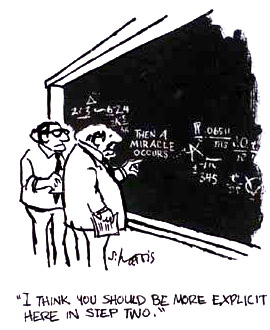
\includegraphics{Math_comic3}
\par\end{center}

\pagebreak{}


\part*{Teorie}

Nejprve se podívejme na notace a triky, budou i dále v textu popsány
a vysvětleny i tam kde se používají, nicméně abychom je poznali a
nebyli nám cizí, uvedeme ty nejzajímavější ihned zde.


\section*{Notace a Triky}
\begin{itemize}
\item $\frac{\partial u}{\partial t}=u_{t}$
\item $\left\Vert u\right\Vert _{A}\leq c\,\&\,\left\Vert u\right\Vert _{B}\leq c\,\Rightarrow\left\Vert u\right\Vert _{A\cap B}\leq c$
\item Trik s polovinou derivace kvadrátu $u_{t}(t)u(t)=\frac{1}{2}\frac{d}{dt}u(t)^{2}$
\item Holderova nerovnost 
\item Poincareho nerovnost
\item Youngova nerovnost $(ab)^{p}\leq\frac{a^{p}}{p}+\frac{b^{p'}}{p'}$,
bez psaní konstant: $(ab)^{p}\overset{\text{Y}}{\lesssim}a^{p}+b^{p'}$
\item $\epsilon$-Young $ab=\sqrt{\epsilon}a\, b/\sqrt{\epsilon}\overset{\text{Y}}{\leq}\epsilon a^{2}/2+b^{2}/(2\epsilon)$
\item Velikost mocněného mnohočlenu lze omezit konstantou krát součtem nejvyšších
mocnin. 
\item $L^{3}\hookrightarrow L^{2}\hookrightarrow L^{1}$ (``$L^{\infty}$
je lepší než $L^{2}$ na omezeném intervalu.'')
\item $W_{(0)}^{-1,2}(\Omega)=(W_{(0)}^{1,2}(\Omega))^{\star}$... zde jako
značení, abychom nemuseli psát hvězdičku. Nutno poznamenat že v jiných
zdrojích se definuje automaticky dole s indexem $_{0}$, takže pozor
na to, může to být matoucí.
\item $u\in W^{k,p}\Rightarrow\nabla u\in W^{k-1,p}$ i kdybysme měli spadnout
do duálu
\item $\triangle\sim\nabla^{2}\Rightarrow(u\in W^{k,p}\Rightarrow\triangle u\in W^{k-2,p})$
i kdybysme měli spadnout do duálu
\item Duál součtu je průnik duálů $A^{\star}+B^{\star}=(A\cap B)^{\star}$
\item Vnořování a hvězdičky - ohvězdičkuju-li vnořené prostory, otočí se
(za jistých předpokladů) vnoření $X\hookrightarrow Y\Rightarrow X^{\star}\hookleftarrow Y^{\star}$.
\item Lebesgueův bod
\item Konvergování součinu
\[
g^{n}\rightharpoonup g\mbox{ v }L^{p}\mbox{ \& }f^{n}\rightarrow f\mbox{ v }L^{p'}\,\Rightarrow\int g^{n}f^{n}\rightarrow\int gf
\]

\end{itemize}

\paragraph*{Vitaliova věta.}

Nechť
\begin{itemize}
\item $Q$ omezená, měřitelná.
\item $f^{n}(x)\rightarrow f(x)$ s.v.
\item Stejná stejnoměrná ekviintegrabilita
\[
\forall\epsilon\,\exists\delta\,\forall n\,\forall\tilde{Q}\subseteq Q:\,|\tilde{Q}|\leq\delta\Rightarrow\int_{\tilde{Q}}|f^{n}(x)|\, dx\leq\epsilon
\]

\end{itemize}
Pak
\[
\lim\int_{Q}f^{n}(x)=\int_{Q}\lim f(x)
\]
Důsledek
\[
f^{n}(x)\rightarrow f(x)\mbox{ s.v. \& existuje }\exists p>1:\,\left\Vert f^{n}\right\Vert _{L^{p}(Q)}\leq c\Rightarrow\lim\int_{Q}f^{n}(x)=\int_{Q}\lim f(x)
\]



\paragraph*{Rozkládání nerovností}

Občas budeme v nerovnostech pokračovat rozložením a následným složením.
Platí li $a+b\leq c$, rozložíme na $a\leq c,\, b\leq c$ a provedeme
nějakou operaci zvětšení $f(a)\leq f(c),\, f(b)\leq f(c)$ a opět
sečteme $f(a)+f(b)\leq2f(c)$. Občas můžeme psát místo $2$ obecnou
konstantu $c$.


\paragraph*{Můžu predepsat i Neumanna i Dirichleta na stejné části hranice?}

Ne, to pak mám moc podmínek. Potom to totiž dopadne tak, že předepíšu
celej gradient na hranici.

Anebo jinak, řekněme že mámerovnici $u''=1$ na $(0,1)$. Když chci
obojí, tak mám zadáno $u(0)=u(1)=u'(0)=u'(1)=0$, ale mám k dispozici
jen dva parametry. Tedy přeurčeno.


\paragraph*{\hypertarget{gronwall}{Gronwall lema}}

Nechť $\eta,\,\beta,\, p$ nezáporné funkce patřící do $L^{1}(0,\, T)$
a $\eta$ AC-spoj splňující $\forall$ s.v. $t\in(0,T)$
\[
\eta'(t)\leq\beta(t)\eta(t)+p(t)
\]
Pak pro $\forall t\in[0,T]$ máme $\eta(t)\leq\exp(\int_{0}^{T}\beta(\tau)\, d\tau)(\eta(0)+\int_{0}^{t}p(\tau)\, d\tau)$


\subparagraph*{Důkaz}

...vynásobením $e^{-\int_{0}^{T}\beta(\tau)\, d\tau}$
\[
\eta'(t)e^{-\int_{0}^{T}\beta(\tau)\, d\tau}\leq\beta(t)\eta(t)e^{-\int_{0}^{T}\beta(\tau)\, d\tau}+p(t)e^{-\int_{0}^{T}\beta(\tau)\, d\tau}
\]
...a zintegrováním:
\[
\int_{0}^{T}\eta'(t)\, dt\,\exp(-\int_{0}^{T}\beta(\tau)\, d\tau)\leq\exp(-\int_{0}^{T}\beta(\tau)\, d\tau)\int_{0}^{T}(\beta(t)\eta(t)+p(t))\, dt
\]





\paragraph*{Gronwall lema s clenem navic}

Nechť $\eta,\,\beta,\, p,\, z$ nezáporné funkce patřící do $L^{1}(0,\, T)$
a $\eta$ AC-spoj splňující $\forall$ s.v. $t\in(0,T)$
\[
z(t)+\eta'(t)\leq\beta(t)\eta(t)+p(t)
\]


Pak pro $\forall t\in[0,T]$ máme $\eta(t)\leq\exp(\int_{0}^{T}\beta(\tau)\, d\tau)(\eta(0)+\int_{0}^{t}p(\tau)\, d\tau)$

dokazu to zase zintegrovanim vyskoci zt se znaminkem

...vynásobením $e^{-\int_{0}^{T}\beta(\tau)\, d\tau}$
\[
\eta'(t)e^{-\int_{0}^{T}\beta(\tau)\, d\tau}\leq\beta(t)\eta(t)e^{-\int_{0}^{T}\beta(\tau)\, d\tau}+p(t)e^{-\int_{0}^{T}\beta(\tau)\, d\tau}
\]
...a zintegrováním:
\[
\int_{0}^{T}z(t)\, dt\int_{0}^{T}\eta'(t)\, dt\,\exp(-\int_{0}^{T}\beta(\tau)\, d\tau)\leq\exp(-\int_{0}^{T}\beta(\tau)\, d\tau)\int_{0}^{T}(\beta(t)\eta(t)+p(t))\, dt
\]




\pagebreak{}


\section*{Bochnerovy prostory}

Funkce budou zobrazovat do $X$ - Banachova prostoru.

\[
C([0,T],\, X):=\{u:\,(0,T)\rightarrow X,\,\text{že }u(t)\,\text{je spojitá}\}
\]



\paragraph*{Slabá měřitelnost}


\paragraph*{Bochnerův integrál}




\section*{Sobolev Bochnerovy prostory}


\paragraph*{Slabá derivace funkce do B.P.}

Nechť X je Banachův, $T>0$, $u\in L^{1}(0,\, T,\, X)$. 

$u_{t}$ je slabá derivace $u$ $\iff$ $\int_{0}^{T}u(t)\,\varphi(t)\, dt=-\int_{0}^{T}u(t)\,\varphi'(t)\, dt\,...\forall\varphi\in D(0,T)$

(Integrál je Bochnerův integrál.)


\paragraph*{Sobolev Bochnerův prostor}

Nechť X je Banachův a $T>0$. Definujeme

\[
W^{1,p}(0,\, T,\, X):=\{u\in L^{p}(0,\, T,\, X),\,\text{slabá derivace }u_{t}\in L^{p}(0,\, T,\, X)\}
\]



\subparagraph*{Vlastnosti\textmd{ $W^{1,p}(0,\, T,\, X)$:}}
\begin{itemize}
\item Banchův pro $\forall p\in[1,\infty]$ s normou: (vlnovkou zdůrazňujeme
zápis ekvivalentní normy) 
\[
||u||_{W^{1,p}(0,\, T,\, X)}=||u||_{L^{p}(0,\, T,\, X)}+||u_{t}||_{L^{p}(0,\, T,\, X)}\sim(||u||_{L^{p}(0,\, T,\, X)}^{p}+||u_{t}||_{L^{p}(0,\, T,\, X)}^{p})^{1/p}
\]

\item Separabilní pokud $p\in[1,\infty)\,\&\, X$ separabilní
\item Reflexivní pokud $p\in(1,\infty)\,\&\, X,\, X^{\star}$ jsou reflexivní
a separabilní
\item Hilbertův pokud $p=2\,\&\, X$ je Hilbertův. Skalární součin je 
\[
(u,\, v)_{W^{1,2}(0,\, T,\, X)}=\int_{0}^{T}(u(t),\, v(t))_{X}\, dt
\]

\end{itemize}

\paragraph*{Vnoření hustota rozšíření}

Nechť X je Banachův a $p\in[1,\infty]$, pak


\subparagraph*{Vnoření
\[
W^{1,p}(0,\, T,\, X)\hookrightarrow C^{0,\,1-1/p}([0,\, T],\, X)
\]
Hustota
\begin{eqnarray*}
\overline{\{C^{\infty}([0,\, T],\, X)\}}\protect\begin{array}{c}
W^{1,p}(0,\, T,\, X)\protect\\
\protect\\
\protect\end{array} & = & W^{1,p}(0,\, T,\, X)\,...\text{pro}\, p<\infty\protect\\
\overline{\{C^{\infty}([0,\, T],\, X)\}}^{\star}\protect\begin{array}{l}
W^{1,p}(0,\, T,\, X)\protect\\
\protect\\
\protect\end{array} & = & W^{1,\infty}(0,\, T,\, X)
\end{eqnarray*}
Rozšíření}

\[
\exists E:\, W^{1,p}(0,\, T,\, X)\rightarrow W^{1,p}(\mathbb{R},\, X)
\]
lineární a omezený (spojitý) operátor, že $\forall u\, Eu(t)=u(t)\,\forall t\in(0,T)$


\subparagraph*{Proč}

Důkazy stejné jako v PDR I, problém je, že nevím jak to zhladit u
hranice. Uvnitř stačí molifikovat, u kraje musim šoupnout aby bydlelo
v $(2\epsilon,\infty)$, teď to mam vně a můžu to zhladit, jde o to
abych se nedostal mimo interval.


\paragraph*{Proč - hustota}

Protože jde o časovou osu, je problém 1D, tedy se rozdělí $u=u_{1}+u_{2}+u_{3}$
(jako rozklad jednotky), kde mají $u_{i}$ kompaktní nosiče v $(0,2\delta),\,(\delta,T-\delta),\,(T-2\delta,T)$.

Rozložené $u_{i}$ molifikujeme (abysme pak mohli znovu sečíst na
$u^{\epsilon}=u_{1}^{\epsilon}+u_{2}^{\epsilon}+u_{3}^{\epsilon}$):
\begin{itemize}
\item $u_{3}$ jednoduše zhladíme rovnou $u_{3}^{\epsilon}:=u_{3}*\eta_{\epsilon}=\int_{\mathbb{R}}u(t)\eta_{\epsilon}(t-\tau)\, d\tau$.
Pak $u_{3}^{\epsilon}\rightarrow u_{3}$ ve $W^{1,p}(0,\, T,\, X)$.
\item $u_{1/2}$ před zhlazením posuneme: $u_{1/2}^{\epsilon}:=u_{1/2}(t+\epsilon)*\eta_{\epsilon}$.
Jak posun tak výsledné zhlazení jde k funkci (protože posouváme ruku
v ruce stejným parametrem jako zhlazujeme). Pak $u_{1/2}^{\epsilon}\in C^{\infty}([0,\infty],\, X)$
a $u_{1/2}^{\epsilon}\rightarrow u_{1/2}$ v $W^{1,p}(0,\, T,\, X)$
\end{itemize}
Mimochodem., kdybych chtěl jen $w^{\star}$ hustotu, tak tohle nemusím
dělat! Pro $w^{\star}$ topologii totiž stačí jen apriorní odhady,
což znamená, že norma tý zhlazený funkce v prostoru co chceme je konečná
a to stačí k tomu, aby to konvergovalo v $w^{\star}$ topologii.


\paragraph*{Proč - vnoření}

K dané $u$ najdeme z hustoty $u^{n}\in C^{\infty}([0,T],\, X)$,
$u^{n}\rightarrow u$ ve $W^{1,p}(0,\, T,\, X)$ (nebo $\rightharpoonup^{\star}$
ve $W^{1,\infty}$ ).

Ukážeme, že $u^{n}$ je cauchyovská ve $C^{0,1-1/p}$ a protože jsme
v Banachprostoru, bude mít limitu.

Pro argumentaci Arzela-Ascoli použijeme stejnou spojitost a stejnou
omezenost. Odhadujeme a koukáme, jestli je výraz malý, kdž jsou $t_{1},\, t_{2}$
blízko:
\[
||u^{n}(t_{2})-u^{n}(t_{1})||_{X}=||\int_{t_{1}}^{t_{2}}u_{t}^{n}(\tau)\, d\tau||_{X}\leq\int_{t_{1}}^{t_{2}}||u_{t}^{n}||_{X}\, d\tau
\]
Pak protože $u^{n}\rightarrow u$ v $W^{1,1}(0,\, T,\, X)$:
\[
\forall\epsilon\exists\delta\forall n:\,|t_{2}-t_{1}|\leq\delta\Rightarrow\int_{t_{1}}^{t_{2}}||u_{t}^{n}||_{X}\, d\tau\leq\epsilon
\]
....Máme tedy stejnou spojitost $||u^{n}(t_{2})-u^{n}(t_{1})||_{X}\leq\epsilon$.
Ještě omezenost - pokud bychom měli pro $t\in[T/2,T]$:
\[
||u^{n}(t)||_{X}\leq||u^{n}(t)-u^{n}(t_{1})||_{X}+||u^{n}(t_{1})||_{X}
\]
Tak pak pomocí Arzela-Ascoli víme, že posloupnost má limitu v prostoru
spojitých funkcí (což jsme chtěli a důkaz by byl ukončený).


\subparagraph{Dokážeme tedy stejnou omezenost: }

První člen $||u^{n}(t)-u^{n}(t_{1})||_{X}$ je $\leq\epsilon$ tzn.
i menší než konstanta, druhý $u^{n}\rightarrow u$ v $L^{1}(0,T,\, X)\Rightarrow\forall\text{(s.v)}\, u^{n}\rightarrow u(t)$
v $X$. Tedy vyberu $t_{1}$ tak, aby platilo že konverguje, díky
čemuž bude taky omezené.

Protože je tedy stejně omezené a stejně spojité, můžu integrovat $dt_{1}$
a zvětšit na celý časový interval: 
\begin{eqnarray*}
\int_{0}^{T/2}||u^{n}(t)||_{X}\, dt_{1} & \leq & \int_{0}^{T/2}||u^{n}(t)-u^{n}(t_{1})||_{X}\, dt_{1}+\int_{0}^{T/2}||u^{n}(t_{1})||_{X}\, dt_{1}\\
 & \leq & c(T)\int_{0}^{T}||u_{t}^{n}||_{X}+||u^{n}||_{X}\, dt_{1}=||u^{n}||_{W^{1,1}(0,T,X)}
\end{eqnarray*}
Levá strana nezávisí na $t_{1}$, proto se rovná: 
\[
||u^{n}||_{W^{1,1}(0,T,X)}\geq\int_{0}^{T/2}||u^{n}(t)||\, dt_{1}=T/2||u^{n}(t)||_{X}
\]
Tohle bylo pro první polovinu intervalu. Pro druhou platí analogicky
a tedy:
\[
\forall t\forall n\,||u^{n}(t)||_{X}\leq c(T)||u^{n}||_{W^{1,1}(0,\, T,\, X)}\rightarrow||u||_{W^{1,1}(0,\, T,\, X)}c(T)
\]
Hotovo, máme omezenost. Tohle bylo vnoření v $W^{1,1}$ v prostoru
spojitejch funkcí.


\subparagraph*{Víc vnoření}

Když máme $W^{1,p}$ pro změnu, tak můžeme vnořit dokonce do Holderovsky
spojitých. Holderovou nerovností máme:

\[
||u^{n}(t_{2})-u^{n}(t_{1})||\leq\int_{t_{1}}^{t_{2}}||u_{t}^{n}||_{X}\, d\tau\leq(\int_{t_{1}}^{t_{2}}||u_{t}^{n}||_{X}^{p})^{1/p}|t_{2}-t_{1}|^{1-1/p}
\]
...a půjdem k limitě (pro $p=\infty$ použiju, že je omezené):
\[
||u^{n}(t_{2})-u^{n}(t_{1})||\leq\int_{t_{1}}^{t_{2}}||u_{t}^{n}||_{X}\, d\tau\leq||u_{t}^{n}||_{W^{1,p}(0,\, T,\, X)}^{p}|t_{2}-t_{1}|^{1-1/p}
\]
...to je přesně definice seminormy. Je to tedy spoj. vnoření (stačí
vydělit $|t_{2}-t_{1}|^{1-1/p}$)


\subsubsection*{Dál}

Doteď jsme dokazovali spojitý vnoření, co se povedlo o $u_{t}\in L^{2}(0,T,\, W_{0}^{1,2}(\Omega)^{\star})\hookrightarrow C([0,T],\, W_{0}^{1,2}(\Omega)^{\star})$
a $u$ je v tomtéž prostoru. Tedy $u$ je spojitá funkce s hodnotama
v tomhle prostoru, ale bodovej význam pro $W_{0}^{1,2}(\Omega)^{\star}$
chybí.
\[
\begin{array}{ccc}
u\in L^{2}(0,T,\, W_{0}^{1,2}(\Omega)^{\star}) & \hookrightarrow & C([0,T],\, L^{2}(\Omega))\\
u_{t}\in L^{2}(0,T,\, W_{0}^{1,2}(\Omega)^{\star}) & ...\Uparrow
\end{array}
\]
Teď můžu říct, že $u$ je spojitá funkce do $L^{2}(\Omega)$. Důvod
je ten, že $L^{2}$ je přesně mezi tutěma prostorama. Dokážeme to
obecně:


\paragraph*{Gelfandova evoluční trojice}

Řekneme, že $X,\, H,\, X^{\star}$ je Gelfandova trojka $\iff X\overset{\text{hustě}}{\hookrightarrow}H=H^{\star}\hookrightarrow X^{\star}$.

$X,\, X^{\star}$ Banachovy, $H$ Hilbertův prostor (``pivot\char`\"{}).


\subparagraph*{Pozn.}

Musí být hustý, jinak neplatí $H^{\star}\hookrightarrow X^{\star}$.
Typicky bude $X=W_{0}^{1,p}(\Omega),\, H=L^{2}$, splňuje předpoklad,
protože hladký funkce jsou hustý v obojím.


\paragraph*{Věta Můžu vnořovat a perpartes na dualitách za jistých předpokladů}

Nechť $X,\, H,\, X^{\star}$ je Gelfandova trojka, pak pro $p\in(1,\infty)$
\begin{itemize}
\item $V:=L^{p}(0,\, T,\, X)\cap W^{1,p'}(0,\, T,\, X^{\star})\hookrightarrow C([0,\, T],\, H)$
\item Navíc $\forall u\,,v\in V\,\forall0\leq t_{1}\leq t_{2}\leq T$ máme
``perpartes\char`\"{}: 
\[
\int_{t_{1}}^{t_{2}}\left\langle u_{t}(t),\, v(t)\right\rangle _{X^{\star},X}+\left\langle v_{t}(t),\, u(t)\right\rangle _{X^{\star},X}\, dt=(u(t_{2}),\, v(t_{2}))_{H}-(u(t_{1}),\, v(t_{1}))_{H}
\]

\end{itemize}

\paragraph*{Pozn.}

Potom dosadíme-li $u=v$, máme:

\[
2\int_{t_{1}}^{t_{2}}\left\langle u_{t}(t),\, u(t)\right\rangle _{X^{\star},X}\, dt=||u(t_{2})||_{H}^{2}-||u(t_{1})||_{H}^{2}
\]
vydělím $t_{2}-t_{1}$ a jdu k limitě:
\[
\Rightarrow\left\langle u_{t}(t),\, u(t)\right\rangle _{X^{\star},X}=1/2\, d/dt\,||u(t)||_{H}^{2}\mbox{ pro s.v. }t\in(0,T)
\]



\paragraph*{Důkaz }

Pomocí hustoty - pro $u\in V$ najdu $u^{n}\rightarrow u$, $u^{n}\in C^{\infty}([0,T],\, X)$
hladký, budu chtít perpartes. Potřebujeme následující vztah:

\framebox{\parbox[t]{1\columnwidth}{%
Rozepíšeme derivaci normy v Hilbertově prostoru a dostaneme dvakrát
časovou derivaci ve skalárním součinu:

\begin{eqnarray*}
\frac{d}{dt}||v(t)||_{H}^{2} & = & \underset{h\rightarrow0}{\lim}\frac{(v(t+h),v(t+h))_{H}-(v(t),v(t))_{H}}{h}\\
 & = & \underset{h\rightarrow0}{\lim}\frac{(v(t+h)-v(t),v(t+h))_{H}}{h}+\frac{(v(t),v(t+h)-v(t))_{H}}{h}\\
 & = & \underset{h\rightarrow0}{\lim}(\frac{v(t+h)-v(t)}{h},v(t+h))_{H}+(v(t),\frac{v(t+h)-v(t)}{h})_{H}\\
 & = & 2(v_{t}(t),\, v(t))_{H}
\end{eqnarray*}


Když výslednou rovnost zintegrujeme $\int_{t_{1}}^{t_{2}}$ a dosadíme
$v(t)=u^{n}(t)-u^{m}(t)$, dostaneme:

\[
||u^{n}(t_{2})-u^{m}(t_{2})||_{H}^{2}=||u^{n}(t_{1})-u^{m}(t_{1})||_{H}^{2}+2\int_{t_{1}}^{t_{2}}(u_{t}^{n}(t)-u_{t}^{m}(t),\, u^{n}(t)-u^{m}(t))_{H}\, dt
\]
%
}}

Vezmeme $t_{2}\in[T/2,T]$, $t_{1}\in[0,T/2]$ a celou rovnost nejprve
změníme na nerovnost - odhadem v absolutních hodnotách a pak odmocníme.
Odmocněnou pravou stranu odhadneme, z toho vylezou konstanty:

(Zbývá ještě dodat, že z definice gelfandovy trojice identifikujeme
skalární součin a dualitu)

\[
||u^{n}(t_{2})-u^{m}(t_{2})||_{H}\leq c(||u^{n}(t_{1})-u^{m}(t_{1})||_{H}+|\int_{t_{1}}^{t_{2}}<u_{t}^{n}(t)-u_{t}^{m}(t),\, u^{n}(t)-u^{m}(t)>_{X^{\star},X}\, dt|^{1/2})
\]


A protože lze vše udělat i obráceně (hozením integrálu na druhou stranu
s mínusem, kde pak mínus zabije ona absolutní hodnota, dostaneme):

\[
-2\int_{t_{1}}^{t_{2}}(u_{t}^{n}(t)-u_{t}^{m}(t),\, u^{n}(t)-u^{m}(t))_{H}\, dt+||u^{n}(t_{2})-u^{m}(t_{2})||_{H}^{2}=||u^{n}(t_{1})-u^{m}(t_{1})||_{H}^{2}
\]


\[
||u^{n}(t_{1})-u^{m}(t_{1})||_{H}\leq c(||u^{n}(t_{2})-u^{m}(t_{2})||_{H}+|\int_{t_{1}}^{t_{2}}<u_{t}^{n}(t)-u_{t}^{m}(t),\, u^{n}(t)-u^{m}(t)>_{X^{\star},X}\, dt|^{1/2})
\]


A první nerovnost zintegrovat k $t_{1}$, druhou k $t_{2}$ - levé
strany se integrací nezmění a přibude pouze konstanta za délku intervalu
\[
||u^{n}(t_{2})-u^{m}(t_{2})||_{H}\leq c(T)(\int_{0}^{T}||u^{n}(t_{1})-u^{m}(t_{1})||_{H}\, dt_{1}+\int_{0}^{T/2}|\int_{t_{1}}^{t_{2}}<u_{t}^{n}(t)-u_{t}^{m}(t),\, u^{n}(t)-u^{m}(t)>_{X^{\star},X}\, dt|^{1/2})\, dt_{1}
\]


A chci ze je cauchyovská $||u^{n}(t)-u^{m}(t)||_{H}\leq\epsilon$
První část je k intervalu {[}0,T/2{]}, druhá část k {[}T/2,T{]} 

 umim cauchyovskost na tech dvou intervalcich a kdyz to umim na dvou
tak to umim na celym a ze prava strana tech nerovnosti je mala se
ukazuje dal

A teď $u^{n}\rightarrow u\, L^{p}(0,\, T,\, X)$ tedy jde silně i
v $L^{1}(0,\, T,\, X)$.

Tedy člen

$\int_{0}^{T}||u^{n}(t_{1})-u^{m}(t_{1})||_{H}\, dt_{1}$ je cauchyovský
ze silny konvergence v prostoru a druhý člen lze odhadnout dualita
a pak Holderem - zase casovou derivaci zvetsime na celej prostor W
(kdybych tam chtel prostor $L$ tak tam musim nechat derivaci dle
času $t$) 
\[
\int_{0}^{T/2}|\int_{t_{1}}^{t_{2}}<...>_{X^{\star},X}\, dt|^{1/2})\, dt_{1}\leq c(T)\int_{0}^{T}||u_{t}^{n}-u_{t}^{m}||_{X^{\star}}||u^{n}-u^{m}||_{X}\, dt\leq c(T)||u^{n}-u^{m}||_{W^{1,p'}(0,T,X^{\star})}||u^{n}-u^{m}||_{L^{p}(0,T,X)}
\]
a to je jistě omezené, ale buď $p=1$ nebo $p'=1$ takže jedna z norem
je omezená a druhá Cauchyovská. Tedy má limitu jako celek.

Takže pro hladké funkce to platí.  zacali sme s tim ze hladky funkce
sou husty pak sme vzali objekt zhladil ia spocitame limitu chci ukazat
ze je cauchyovska v tom spravnym prostoru kdyz v jednom z nich mame
hustotu tak sme vyhrali!

Je snadná cesta ke kompaktnímu vnoření - pro regularitu $u\in L^{2}(0,T,W^{1,2}),\, u_{t}\in L^{2}(0,\, T,L^{2})$,
z toho bysme měli

$\hookrightarrow\hookrightarrow L^{2}((0,T)\times\Omega)$. To ale
často nemáme.


\paragraph*{Věta Aubin Lions Roubíček}

Nechť $X,\, Y,\, Z$ Banachprostory, $X\hookrightarrow\hookrightarrow Y\hookrightarrow Z$
(separabilní, (reflexivní)), $p\in(1,\infty)$. Pak
\[
V:=L^{p}(0,T,X)\cap W^{1,1}(0,T,\, Z)\hookrightarrow\hookrightarrow L^{p}(0,T,\, Y)
\]
Pozn - Roubíček: stačí radonovy míry a $Z$ lokálně konvexní.


\paragraph*{Důkaz A-L-R}

Chceme sekvenční kompaktnost - pro $u^{n}$ omezenou ve $V$ najít
$u^{n_{k}}\rightarrow u$ v $L^{p}(0,T,\, Y)$.

Nejdřív použijeme že $X$ reflexivní - můžeme najít (BÚNO s přechodem
k podposloupnosti) $u^{n}\rightharpoonup u\,\text{v }L^{p}(0,T,\, X)$
(...který je díky $X$ také reflexivní).


\subparagraph*{Ehrlingovo lemma}

Nechť $X\hookrightarrow\hookrightarrow Y\hookrightarrow Z$ (reflexivní,
Banachprostory), pak
\[
\forall a>0\,\exists c(a)\,\forall u\in X:\,\left\Vert u\right\Vert _{Y}\leq a\left\Vert u\right\Vert _{X}+c(a)\left\Vert u\right\Vert _{Z}
\]



\subparagraph*{Důkaz Ehrlinga}

Důvod proč to můžeme udělat je právě kompaktní vnoření. Sporem - nechť
\[
\exists a>0\,\forall n\,\exists u^{n}\mbox{, že }\left\Vert u^{n}\right\Vert _{Y}=1
\]
 (búno normalizujeme) a neplatí závěr, tedy 

\[
1=\left\Vert u^{n}\right\Vert _{Y}>a\left\Vert u^{n}\right\Vert _{X}+n\left\Vert u^{n}\right\Vert _{Z}
\]
Protože je omezené v $X$, které je kompaktně vnořené do $Y$ (a do
$Z$), platí (pro podposloupnost) $u^{n}\rightarrow u$ v $Y$ (a
v $Z$; to je důležité k tomu, že limita v těchto prostorech existuje):
\[
\Rightarrow\,1>n\left\Vert u^{n}\right\Vert _{Z}\Rightarrow\left\Vert u^{n}\right\Vert _{Z}\rightarrow0\Rightarrow u^{n}\rightarrow0\text{ v }Z\Rightarrow u=0
\]
...ale to je spor: $u=0\,\times\,\left\Vert u^{n}\right\Vert _{Y}=1$


\subparagraph*{Pokračování důkazu A-L-R}

Ukážeme, že $u^{n}$ je cauchyovská v $L^{p}$ k $Y$. Odhady ($a$
je libovolné, což bude důležité, protože ho dál budeme šikovně volit)
\[
\left\Vert u^{n}(t)-u^{m}(t)\right\Vert _{Y}\overset{\text{Ehrlingovo lemma}}{\leq}a\left\Vert u^{n}(t)-u^{m}(t)\right\Vert _{X}+c(a)\left\Vert u^{n}(t)-u^{m}(t)\right\Vert _{Z}
\]
teď umocníme na $p$, použijeme že umocněné sčíance lze omezit konstantou
krát nejvyššími členy a zintegrujeme přez čas:

Člen $\int_{0}^{T}||u^{n}(t)-u^{m}(t)||_{X}^{p}$ se schová do konstanty,
protože je posl z předpokladu omezená ve $V$ (... a tedy je omezená
i v $X$, protože je tam integrál přez čas z normy $X$ a ten sedí
v týhle části prostoru $V$: ``$L^{p}(0,T,X)\cap$'').

\begin{eqnarray*}
\int_{0}^{T}\left\Vert u^{n}(t)-u^{m}(t)\right\Vert _{Y}^{p} & \leq & c(p)(a\int_{0}^{T}\left\Vert u^{n}(t)-u^{m}(t)\right\Vert _{X}^{p}\, dt+c(a)\int_{0}^{T}\left\Vert u^{n}(t)-u^{m}(t)\right\Vert _{Z}^{p}\, dt)\\
\mbox{(schoval se)} & \leq & a\, c(p)+c(a,p)\int_{0}^{T}\left\Vert u^{n}(t)-u^{m}(t)\right\Vert _{Z}^{p}\, dt\\
\text{(zvolíme }a=\frac{\epsilon}{3c(p)}:\mbox{)} & \leq & \frac{\epsilon}{3}+c(\epsilon,p)\int_{0}^{T}\left\Vert u^{n}(t)-u^{m}(t)\right\Vert _{Z}^{p}\, dt
\end{eqnarray*}
Kompaktnost posledniho clenu (v $L^{p}(Z)$, kterou dokážeme níže)
zaručí odhadnutelnost $\epsilon/3,\, c(\epsilon,p)$ bude sice velké,
ale to vyřešíme právě konvergencí posledního členu. Pro ten zavedeme
aproximaci a budeme směřovat k odhadu, který použije fakt, že kontrolujeme
časovou derivaci. Aproximaci zavedeme takto:\\
\framebox{\parbox[t]{1\columnwidth}{%
\[
\delta>0:\, u_{\delta}^{n}(t)=1/\delta\int_{0}^{\delta}u^{n}(t+\tau)\, d\tau
\]
(...střední hodnota. Hladké pro fixní $\delta$. Je Bochnerův integrál.)
Použijeme tuhle aproximaci a dosadíme (pro trojúhelníkovou nerovnost):%
}}

\[
\int_{0}^{T}\left\Vert u^{n}(t)-u^{m}(t)\right\Vert _{Y}^{p}\leq...\leq\frac{\epsilon}{3}+c(\epsilon,\, p)\int_{0}^{T}\left\Vert u_{\delta}^{n}-u_{\delta}^{m}\right\Vert _{Z}^{p}\, dt+c(\epsilon,\, p)\underline{\int_{0}^{T}\left\Vert u^{n}-u_{\delta}^{n}-(u^{m}-u_{\delta}^{m})\right\Vert _{Z}^{p}}_{\text{[Tohle]}}\, dt\leq
\]
...A teď zvážit, jak zvolit $\delta$ , aby {[}Tohle{]} bylo malé.\\
\framebox{\parbox[t]{1\columnwidth}{%
Budu odhadovat $u^{n}-u_{\delta}^{n}$. ($u^{n}$ nezávísí na čase
a na $u_{\delta}^{n}(t)$ použijeme vzoreček. Mínus přibude z toho,
že dáme časovou derivaci. Předposledním rovnítkem si připravíme chytře
derivaci pro perpartes. Poslední rovnítko je perpartes, kde je hraniční
člen nulový - pro $\tau=\delta$ je nula jeden, pro $\tau=0$ druhý.)
\begin{eqnarray*}
u^{n}(t)-u_{\delta}^{n}(t) & = & \frac{1}{\delta}\int_{0}^{\delta}u^{n}(t)-u^{n}(t+\tau)\, d\tau=\frac{-1}{\delta}\int_{0}^{\delta}\int_{0}^{\tau}u_{t}^{n}(s+t)\, ds\, d\tau=\\
 & = & -\int_{0}^{\delta}((\frac{\tau}{\delta}-1)_{\tau}\int_{0}^{\tau}u_{t}^{n}(t+s)\, ds)\, d\tau=+\int_{0}^{\delta}(\frac{\tau}{\delta}-1)u_{t}^{n}(t+\tau)\, d\tau+0
\end{eqnarray*}
Vezmeme odvozenou rovnost v normě a dostaneme nerovnost (vytknutím
z normy prohodíme pořadí $\frac{\tau}{\delta}-1$, aby bylo kladné).
Je omezené konstantou, protože $1-\frac{\tau}{\delta}$ je omezené
a integruju dle času a ten je dle předpokladu v $L^{1}$, tedy omezený:
\begin{align}
\left\Vert u^{n}(t)-u_{\delta}^{n}(t)\right\Vert _{Z} & \leq\int_{0}^{\delta}(1-\frac{\tau}{\delta})\left\Vert u_{t}^{n}(t+\tau)\right\Vert _{Z}\, d\tau\leq const(\left\Vert u_{t}\right\Vert _{L^{1}(0,T,Z)}+1)\tag{1, odhad v Z}\label{eq:dostanemener}
\end{align}
Nerovnost platí pro libovolný čas.

Chceme odhadnout $c(\epsilon,\, p)\int_{0}^{T}\left\Vert u^{n}-u_{\delta}^{n}-(u^{m}-u_{\delta}^{m})\right\Vert _{Z}^{p}$,
část toho členu budeme odhadovat takhle:
\[
c(\epsilon,\, p)\int_{0}^{T}\left\Vert u^{n}-u_{\delta}^{n}\right\Vert _{Z}^{p}\, dt=c(\epsilon,\, p)\int_{0}^{T}\left\Vert u^{n}-u_{\delta}^{n}\right\Vert _{Z}^{p-1}\left\Vert u^{n}-u_{\delta}^{n}\right\Vert _{Z}\, dt\leq
\]
...Rozdělili sme si na mocniny, abychom mohli udělat následující úvahu:
protože fce je z $W^{1,1}$ s hodnotama v prostoru $Z$, tak je i
v $L^{\infty}$ s hodnotama v prostoru $Z$ (na omezeném intervalu
je vnořená do spojitých funkcí a ty jsou integrovatelné), takže to
můžu odhadnut normou $L^{\infty}$ přez čas. A to je podle předpokladu
na prostory omezené, konstanta. Odhadujeme jen $p-1$ mocnin, protože
sice můžeme odhadnout celé, ale zbytek chceme ukázat, že půjde do
nuly (a takhle bysme dostali jen omezenost konstantou).

...dále použijeme odvozenou (\ref{eq:dostanemener}):
\[
\leq c(\epsilon,\, p)\int_{0}^{T}\left\Vert u^{n}-u_{\delta}^{n}\right\Vert _{Z}\, dt\leq c(\epsilon,\, p)\int_{0}^{T}\int_{0}^{\delta}(1-\tau/\delta)\left\Vert u_{t}^{n}(t+\tau)\right\Vert _{Z}\, d\tau\, dt=
\]
Fubi:
\[
=c(\epsilon,\, p)\int_{0}^{\delta}(1-\tau/\delta)\underline{\int_{0}^{T}\left\Vert u_{t}^{n}(t+\tau)\right\Vert _{Z}\, dt}\, d\tau\leq c(\epsilon,\, p)\int_{0}^{\delta}(1-\tau/\delta)\, d\tau\leq\delta c(\epsilon,p)
\]


Předposlední nerovnítko platí protože nejdřív integruju přez $t$
a podtrženou věc uvnitř odhadnu konstantou, protože je omezená dle
předpokladů. (Nutno poznamenat, že se dostávám mezí integrálu nad
$T$, ale je tam věta o rozšíření, že to můžu prodloužit.)%
}}

Tzn. dostanu $\epsilon$, najdu $a=\epsilon/(3c(p))$, vybereme $\delta$,
aby $\delta c(\epsilon,\, p)<\epsilon$ a tedy $\delta:=\epsilon/(6c(\epsilon,\, p))$.
Pokračujeme. Delta teď bude dané pomocí epsilon a fixní:
\[
\leq\frac{\epsilon}{3}+c(\epsilon,\, p)\int_{0}^{T}\left\Vert u_{\delta(\epsilon)}^{n}-u_{\delta(\epsilon)}^{m}\right\Vert _{Z}^{p}\, dt+\underline{\frac{\epsilon}{3}}_{\text{[Tohle]}}\leq
\]
...Doteď nic nezáviselo na $n,\, m$, to přijde teď:\\
\framebox{\parbox[t]{1\columnwidth}{%
Máme tři fakta:
\begin{itemize}
\item Vzpomeneme na $u_{\delta}^{n}(t):=1/\delta\int_{0}^{\delta}u^{n}(t+\tau)\, d\tau$ 
\item přidáme fakt ze začáku důkazu - že $u^{n}\rightharpoonup u\text{ v }L^{p}(0,T,\, X)$
\item a máme kompaktní vnoření $X\hookrightarrow\hookrightarrow Z$
\end{itemize}
Z toho existuje limitní $\forall t\, u_{\delta}^{n}(t)\rightarrow u_{\delta}$
v $Z$ - ze slabé konvergence. je to boch int a jde to slabe . (Pro
každý čas $t$ je to omezené v $X$ a $X$ kompaktně vnořené do $Z$,
takže pro každý $t$ pevný to konverguje silně v $Z$. Dál už jenom
ukážeme, že stejnoměrná.)%
}}

...Pomocí toho odhadneme druhý člen, dostaneme tam trojúhelníkovou
nerovností limitu: 
\[
\leq\frac{2\epsilon}{3}+c(\epsilon,\, p)\int_{0}^{T}\left\Vert u_{\delta(\epsilon)}^{n}-u_{\delta}\right\Vert _{Z}^{p}+\left\Vert u_{\delta(\epsilon)}^{m}-u_{\delta}\right\Vert _{Z}^{p}\, dt\leq
\]
...Najdeme $n,\, m\geq n_{0}$ aby byl poslední zbývající člen $\leq\epsilon/3$.\\
\framebox{\parbox[t]{1\columnwidth}{%
$\epsilon,\,\delta$ dané a fixní, tedy jdeme k limitě.

\[
\lim_{n\rightarrow\infty}\int_{0}^{T}\left\Vert u_{\delta(\epsilon)}^{n}-u_{\delta}\right\Vert _{Z}^{p}\underset{\text{\text{věta}}}{\overset{\text{Lebesgueova}}{\text{=}}}\int_{0}^{T}\lim_{n\rightarrow\infty}\left\Vert u_{\delta(\epsilon)}^{n}-u_{\delta}\right\Vert _{Z}^{p}\, dt=0
\]


Můžu najít integrovatelnou majorantu, protože je omezené konstantou
($\left\Vert u_{\delta}^{n}\right\Vert _{Z}\leq1/\delta\int_{0}^{T}\left\Vert u^{n}(t+\tau)\right\Vert _{Z}\, d\tau\leq c/\delta$).

No a když ta limita je nula, tak lze rozhodně ``najít $n,\, m\geq n_{0}$
aby byl poslední zbývající člen $\leq\epsilon/3$\char`\"{}.%
}}

\[
\leq\frac{2\epsilon}{3}+\frac{\epsilon}{3}
\]


A protože je Banachprostor a posloupnost je Cauchyovská, tak konverguje.\pagebreak{}


\section*{Spojitý svět}

Ukážeme si hyperbolickou a parabolickou rovnici a budeme předpokládat
takovou spojitost, že všechny úpravy (násobení, integrování, derivování)
lze dělat. Dělám to proto, abych viděl jak se rovnice chovají ve spojitém
přpadě a co všechno můžu udělat. Navíc z toho pak lze vykoukat prostory
funkcí (protože i pro spojitý se může ukázat, že nemají hladký řešení).

Pak zkusíme budovat teorii tak, abysme dostali co nejvíc výsledků
jako pro spojitý případ. 

To je matematický přístup. Fyzikálně se na to lze koukat tak, abysme
viděli kde problém vzniknul a o co rovnice popisuje, protože pak třeba
víme, že data splňují rovnice pro zachování energie (a teorie lze
vybudovat z předpokladu, že energie se zachová i v celém evolučním
procesu).


\paragraph*{Evoluční rovnice}

Se jmenují evoluční, protože přidáme časovou derivaci. Půjde pak o
hyberbolické rovnice (druhá časová derivace) a parabolické rovnice
(první časová derivace).


\paragraph*{Přicházení na prostory a chápání dualit}

V průběhu dalších úprav a úvah budeme odvozovat kam která funkce patří
do jakých prostorů. Dá se říct, že tím, že přibude časová derivace
se prostor zesložití. Například pro jednoduchou rovnici si lze laplace
přepsat a hodit na druhou stranu:
\begin{eqnarray*}
u_{t}-\triangle u & = & 0\\
u_{t} & = & div(\nabla u)
\end{eqnarray*}
No a když, jako v PDR I eliptickém případě předpokládáme, že $\nabla u\in L^{2}(L^{2})$,
pak je $u_{t}$ z duálního prostoru $u_{t}\in L^{2}(0,T,W_{0}^{-1,2})$.
Proč - protože dualitu chápeme takhle:
\[
\left\langle u_{t},\varphi\right\rangle =\left\langle div\,\nabla u,\varphi\right\rangle =-\left\langle \nabla u,\nabla\varphi\right\rangle =\int_{\Omega}\nabla u\nabla\varphi\, dx
\]
(Rovnost $\left\langle div\,\nabla u,\varphi\right\rangle =-\left\langle \nabla u,\nabla\varphi\right\rangle $
platí z hladkosti.)

Ptáme se, pro jaké $\varphi$ má pravá strana smysl (známe li $\nabla u\in L^{2}$).
Musí být z prostoru $\nabla\varphi\in L^{2}(0,T,L^{2}(\Omega))$ (vnitřní
$L^{2}$ protože hodnoty vystupují v dualitě, vnější protože chceme
integrovat i přez čas, tedy musí být nějaký $L$ prostor a volíme
optimální jako duální k prostoru, ve kterém je $\nabla u$. Protože
je $\nabla u\in L^{2}(L^{2})$, je dualita také $L^{2}$ (kdyby bylo
$p$ tak je $p'$)).

To znamená, že $\varphi\in L^{2}(0,T,W_{0}^{1,2}(\Omega))$. 

To zpětně pro levou stranu musí znamenat, že $u_{t}\in(L^{2}(0,T,W_{0}^{1,2}(\Omega)))^{\star}$,
kde je prostor dle věty z B-S prostorů rovno $u_{t}\in L^{2}(0,T,W_{0}^{-1,2}(\Omega))$
(duál se přenesl dovnitř).


\paragraph*{Testovačka je z duálu}

Když $u-u_{D}\in P_{0}$ (obecný prostor), tak testovací funkce musí
být z prostoru duálního $P_{0}^{\star}$ (a samozřejmě obráceně).


\paragraph*{Duality}

Z věty B-P - když máme $X\hookrightarrow H\hookrightarrow X^{\star}$,
pak pro $u,\varphi\in X$ platí $\left\langle u,\varphi\right\rangle _{X,X^{\star}}=(u,\varphi)_{H}$,
to ale pouze v případě, kdy $\varphi\in X$. Pak je z vnoření i v
$X^{\star}$ a lze dosadit do duality, nicméně rovnost se skalárním
součinem je z věty pouze když bylo původně v $X$.


\paragraph*{Duality podruhé}

Pokud máme $u\in W_{0}^{-1,2}$, pak lze zapsat (tzn $\exists f$)
takto: $u=div\, f,\, f\in L^{2}(\Omega,R^{d})$.

Protože můžu spočítat rovnici $-\triangle v=0$, vyřeším a vím $div\,\nabla v=u$
a vezmu $f=\nabla v$.


\subsubsection*{Ještě jednou a lidsky}

Obecně apriorní odhady dají výsledek pro prostor: 
\[
\mbox{Tvar }div(A(u)\nabla u)\Rightarrow L^{\infty}(0,T,L^{2}(\Omega))\cap L^{2}(0,T,W^{1,2}(\Omega))
\]


Jak tyhle výsledky dají? Odvodím-li odhad tvaru (lépe řečeno chci
odvodit takový odhad v příkladech) $\int_{0}^{T}\left\Vert u\right\Vert _{{\color{blue}X}}^{{\color{red}p}}\leq c$,
pak z toho budu mít, že $u\in L^{{\color{red}p}}(0,T,{\color{blue}X})$.
Proč - protože mám li samotnou nerovnost $\int_{0}^{T}\mbox{něco}^{p}\leq c$,
pak $\mbox{něco}\in L^{p}(0,T)$. Když je něco navíc funkce, a znám
odhad v normě přez čas, tak už náleži do prostoru časových zobrazení
do funkcí.


\paragraph*{Jak prostor pro $u_{t}$}

Jakmile mám prostor, ze kterého beru řešení, potřebuju najít prostor
pro $u_{t}$ (nebo $u_{tt}$ pro hyperbolickou). Platí následující
pravidlo:


\paragraph*{Často}

Pokud $u\in S$, $S$ je nějaký prostor, pak $u_{t(t)}\in S^{\star}$
- v duálu k nějakému prostoru.


\paragraph*{Detailní postup}

(který je důkazem tvrzení ``Často'' a vysvětluje co dělat, pokud
nejsme v Častém případu) je takový, že jakmile známe prostor pro $u$
(a rozhodli jsme se nějak i pro $u_{0}$ a $f$, nebo je máme zadané),
přepíšeme si rovnici tak, že na levé straně necháme jen $u_{t(t)}$
a na pravou stranu dáme vše ostatní. A ptám se, kam náleží pravá strana
jako celek. Použijeme k tomu následující pravidla:
\begin{itemize}
\item $u\in W^{k,p}\Rightarrow\nabla u\in W^{k-1,p}$
\item $\triangle\sim\nabla^{2}\Rightarrow(u\in W^{k,p}\Rightarrow\triangle u\in W^{k-2,p})$
\item $W^{-\mbox{něco},\mbox{něco}}$ je duál a je to vymyšlené tak, aby
předchozí dva řádky spadly do duálu
\item Duál součtu je průnik duálů $A^{\star}+B^{\star}=(A\cap B)^{\star}$
\end{itemize}
\pagebreak{}


\subsection*{Rovnice vlny a vedení tepla}

Initial boundary value problem.

Máme $T>0$, $\Omega\subseteq\mathbb{R}^{d}$ otevřenou, omezenou.
\[
\begin{array}{lrr}
f: & (0,T)\times\Omega\rightarrow\mathbb{R}\\
u_{D}: & (0,T)\times\Gamma_{D}\rightarrow\mathbb{R} & (\Gamma_{D}\subseteq\delta\Omega)\\
\sigma: & (0,T)\times\Gamma_{N}\rightarrow\mathbb{R} & (\Gamma_{N}\subseteq\delta\Omega)\\
K: & (0,T)\times\Gamma_{N}\rightarrow\mathbb{R}
\end{array}
\]
Cíl - najít $u:\,(0,T)\times\Omega\rightarrow\mathbb{R}$.


\paragraph*{Rovnice tepla - parabolická}

\[
\begin{array}{rcll}
u_{t}-\triangle u & = & f & \textrm{v}\, Q_{T}:=(0,T)\times\Omega\\
u & = & u_{D} & \textrm{v}\,(0,T)\times\Gamma_{D}\\
\frac{\partial u}{\partial n}+\sigma u & = & K & \textrm{v}\,(0,T)\times\Gamma_{N}\\
u(0,x) & = & u_{0}(x) & \textrm{s.v. v }\Omega
\end{array}
\]



\paragraph*{Rovnice vlny - hyperbolická}

\begin{equation*}
\begin{aligned}[c] 
u_{tt}-\triangle u &=f &...\textrm{v}\, Q_{T}:=(0,T)\times\Omega \\
u&=u_{D}\,&...\textrm{v}\,(0,T)\times\Gamma_{D} \\
\frac{\partial u}{\partial n}+\sigma u&=K\,&...\textrm{v}\,(0,T)\times\Gamma_{N} \\
u(0,x)&=u_{0}(x)\,&...\,\textrm{s.v. v }\Omega \\
u_{t}(0,x)&=v_{0}(x)\,&...\,\textrm{s.v. v }\Omega \\
\end{aligned}
\end{equation*} 


\paragraph*{Rozdíl v těch rovnicích je v kvadratickém členu. V propagaci.}

Konkrétní důsledky:
\begin{enumerate}
\item Vlnová rovnice nevidí časový směr, rovnice tepla ano.
\item Rovnice tepla má vlastnost zhlazení. Zatímco vlnová rovnice propaguje
singularity. Pro lineární hyberbolický rovnice 2. řádu lze říct, že
když je stav zpočátku hladký, tak hladký zůstane. Ale to jen pro linearní
hyperbolický. Když nejsou hladký, tak nezkončím s hladkejma, protože
nemá zhlazovací vlastnost - nespojitosti se přenášej.
\item Rovnice tepla jde do equilibria pro $t\rightarrow\infty$. Vlny ne.
\end{enumerate}

\paragraph*{Vlnová rovnice a časový směr}

Zavedeme $\tilde{u}(t)=u(T-t)$, resp se značením ($f(t)\simeq f(t,x),\, f:\,(0,T)\rightarrow X\,\textrm{- B.P.}$)
je to i funcke prostoru. A řeší vlnovou rovnici - dosazením a zderivováním
(znamínko se dvojzderivováním zruší):
\begin{eqnarray*}
\tilde{u_{tt}}(t)-\triangle\tilde{u}(t) & = & u_{tt}(T-t,x)-\triangle u(T-t,x)=f(T-t,x)\\
\tilde{u} & = & 0\,\textrm{na }(0,T)\times\Gamma_{D}
\end{eqnarray*}
... tj. dle předpokladu nula na okraji a zbývá dodat počpodmínku $\tilde{u}(0)=u(T-0)=u(T)$.
Pak $\tilde{u_{t}}(0)=-u_{t}(T-0)=-u_{t}(T)$. To znamená, že umím-li
vyřešit problém pro počáteční stav, umím i dostat počáteční stav z
koncového stavu (tou samou rovnicí, jen se substitucí).


\paragraph*{Rovnice tepla a časový směr}

Podobné úpravy ale s jiným závěrem:
\[
\begin{array}{rcl}
\tilde{u_{t}}(t)+\triangle\tilde{u}(t) & = & -u_{t}(T-t,x)+\triangle u(T-t,x)=-f(T-t,x)\\
\tilde{u} & = & 0\,\textrm{na }(0,T)\times\Gamma_{D}\\
\tilde{u}(0) & = & u(T-0)=u(T)
\end{array}
\]
Tedy když obrátíme tok času, tak se rovnice změní - mínus pravá strana!
Proto se tohle jmenuje zpětná rovnice tepla.

Když tam mám $-\triangle u$ jdu dopředu s časem, když tam mám $+\triangle u$,
jdu z finálního dozadu.


\paragraph*{Zhlazení a dosažení equilibira}

K těmto faktům se dostaneme pomocí apriorních odhadů.


\subparagraph*{Jak to udělat - první apriorní odhad}
\begin{itemize}
\item rovnice tepla - testujeme pomocí $u$
\item rovnice vlny - testujeme pomocí $u_{t}$
\end{itemize}

\subsubsection*{Aprioriní odhad rovnice tepla}

Budeme odhadovat normy $u$ a $u_{t}$.


\paragraph*{Odhad pro $u$}

Vynásobíme (``otestujeme\char`\"{}) $u(t)$ s fixním $t$ a zintegrujeme:
\[
\int_{\Omega}u_{t}(t)\, u(t)-\triangle u(t)\, u(t)\, dx=\int_{\Omega}f\, u(t)\, dx
\]
...přepíšeme:
\[
\int_{\Omega}1/2\,\frac{d}{dt}|u(t)|^{2}+|\nabla u(t)|^{2}\, dx=\left\langle f(t),\, u(t)\right\rangle _{(W_{0}^{1,2}(\Omega))^{\star},W_{0}^{1,2}(\Omega)}
\]
...a dostáváme rovnici energie:
\[
1/2\,\frac{d}{dt}||u(t)||_{2}^{2}+||\nabla u(t)||_{2}^{2}=\left\langle f(t),\, u(t)\right\rangle 
\]
Apriorní odhad odvodíme z rovnice energie pomocí nerovnosti na pravou
stranu:
\begin{align}
\left\langle f(t),\, u(t)\right\rangle  & \leq||f(t)||_{(W_{0}^{1,2})^{\star}}||\nabla u(t)||_{1,2}\nonumber \\
 & \leq\frac{||f(t)||_{2}^{2}}{2}+\frac{||\nabla u(t)||_{2}^{2}}{2} & \tag*{2,\ensuremath{\left\langle f(t),\, u(t)\right\rangle \leq}...}\label{eq:Poincare1}
\end{align}
(Poincarého nerovností jsme upravili dualitu a použili Youngovu nerovnost.)

Nerovnost aplikujeme na pravou stranu, po přesunu členu s gradientem
na levou stranu dostaneme všude poloviny, takže po vynásobení dvěma:
\begin{equation}
\frac{d}{dt}||u(t)||_{2}^{2}+||\nabla u(t)||_{2}^{2}\leq||f(t)||_{(W_{0}^{1,2})^{\star}}^{2}\tag{3, odhad z rovnice energie}\label{eq:odhadzrceenergie}
\end{equation}
...což zintegrujeme od $0$ do $t_{0}$, člen s $u(0)$ dáme na pravou
stranu (protože se jedná o počáteční podmínku):
\begin{eqnarray*}
||u(t_{0})||_{2}^{2}+\int_{0}^{t_{0}}||\nabla u(t)||_{2}^{2}\, dt & \leq & \int_{0}^{t_{0}}||f(t)||_{(W_{0}^{1,2})^{\star}}^{2}\, dt+||u(0)||_{2}^{2}\\
||u(t_{0})||_{2}^{2} & \leq & \int_{0}^{t_{0}}||f(t)||_{(W_{0}^{1,2})^{\star}}^{2}\, dt+||u(0)||_{2}^{2}\\
\int_{0}^{t_{0}}||\nabla u(t)||_{2}^{2}\, dt & \leq & \int_{0}^{t_{0}}||f(t)||_{(W_{0}^{1,2})^{\star}}^{2}\, dt+||u(0)||_{2}^{2}
\end{eqnarray*}
...spodní dva řádky dostaneme z řádky první, protože oba členy na
levé straně jsou nezáporné a odhadlé pravou stranou. A protože platí
nerovnost $\forall t_{0}\in(0,T)$, zvětšíme integrály až do $T$
a v druhé nerovnosti budeme moct psát supremum. Protože se jedná o
$L^{1}$ prostory, píšeme esssup (hodnota v bodě by neměla smysl psát).
Sečtením dostaneme následující nerovnost:
\begin{align}
\underset{t\in(0,T)}{essup}||u(t)||_{2}^{2}+\int_{0}^{T}||\nabla u(t)||_{2}^{2}\, dt & \leq2(\int_{0}^{T}||f(t)||_{(W_{0}^{1,2})^{\star}}^{2}\, dt+||u_{0}||_{2}^{2})\tag{4, esssup pro u}\label{eq:essupprou}
\end{align}
...použijeme Poincarého/Friedrichsovu nerovnost a normu gradientu
zmenšíme ekvivalentně na celou normu prostoru $W_{0}^{1,2}$:
\[
\underset{t\in(0,T)}{essup}||u(t)||_{2}^{2}+\frac{1}{c}\int_{0}^{T}||u(t)||_{W_{0}^{1,2}}^{2}\, dt\leq2(\int_{0}^{T}||f(t)||_{(W_{0}^{1,2})^{\star}}^{2}\, dt+||u_{0}||_{2}^{2})
\]
...což zapsáno v normách Bochnerových prostorů: 
\begin{itemize}
\item $esssup$ přez čas z kvadrátu $L^{2}$ normy je norma $L^{\infty}(0,\, T,\, L^{2}(\Omega))$,
\item $\int_{0}^{T}||u(t)||_{W_{0}^{1,2}}^{2}\, dt$ je norma $L^{2}(0,\, T,\, W_{0}^{1,2}(\Omega))$
\item stejně tak integrál přez čas z kvadrátu normy duálu je norma $L^{2}(0,\, T,\,(W_{0}^{1,2}(\Omega))^{\star})$):
\end{itemize}
Dává
\[
||u(t)||_{L^{\infty}(0,\, T,\, L^{2}(\Omega))\cap L^{2}(0,\, T,\, W_{0}^{1,2}(\Omega))}^{2}\leq c(dim,\Omega)(||u_{0}||_{2}^{2}+||f||_{L^{2}(0,\, T,\,(W_{0}^{1,2}(\Omega))^{\star})}^{2})
\]
(Kvadráty norem v odhadu se přenesly na kvadrát normy v Bochner-Sobolevově
prostoru.)


\paragraph*{Odhad pro $u_{t}$}

Rovnici $u_{t}=\triangle u+f$ dosadíme do vyjádření normy derivace
(druhá rovnost), rozdělíme a pomocí parpartes hodíme laplace na gradient
na oba členy $u$ i testovací $\varphi$ (třetí rovnost):
\begin{align*}
||u_{t}(t)||_{(W_{0}^{1,2}(\Omega))^{\star}} & = & \sup_{\begin{array}{c}
\varphi\in W_{0}^{1,2}(\Omega)\\
||\varphi||\leq1
\end{array}}\left\langle u_{t}(t),\,\varphi\right\rangle  & = & \sup\left\langle \triangle u(t)+f,\,\varphi\right\rangle =\\
 & = & \sup\left\langle f(t),\,\varphi\right\rangle -\int_{\Omega}\nabla u(t)\,\nabla\varphi & \leq & ||f(t)||_{(W^{1,2}(\Omega))^{\star}}+||\nabla u(t)||_{2}
\end{align*}
Umocněním na druhou a AG nerovností:
\[
||u_{t}(t)||_{(W_{0}^{1,2}(\Omega))^{\star}}^{2}\leq2(||f(t)||_{(W^{1,2}(\Omega))^{\star}}^{2}+||\nabla u(t)||_{2}^{2})
\]
Zintegrujeme od $0$ do $T$:
\[
\int_{0}^{T}||u_{t}(t)||_{(W_{0}^{1,2}(\Omega))^{\star}}^{2}\, dt\leq2\int_{0}^{T}(||f(t)||_{(W^{1,2}(\Omega))^{\star}}^{2}+||\nabla u(t)||_{2}^{2})\, dt
\]
Vzpomeneme na nerovnost \ref{eq:essupprou} výše:{\scriptsize{
\[
\left(\underset{t\in(0,T)}{essup}||u(t)||_{2}^{2}+\underline{\int_{0}^{T}||\nabla u(t)||_{2}^{2}\, dt\leq2(\int_{0}^{T}||f(t)||_{(W_{0}^{1,2})^{\star}}^{2}\, dt+||u_{0}||_{2}^{2})}\right)
\]
}}..a podtrženou část dosadíme na pravou stranu za $||\nabla u(t)||_{2}^{2}$:
\[
\leq4\int_{0}^{T}(||f(t)||_{(W^{1,2}(\Omega))^{\star}}^{2}\, dt+||u_{0}||_{2}^{2})
\]
Právě nám přibyl odhad na $||u_{t}||_{L^{2}(0,\, T,\, W_{0}^{-1,2}(\Omega))}^{2}$.
Z předchozího (``odhad pro $u$\char`\"{}) máme odhadlé i normy $||u(t)||_{L^{\infty}(0,\, T,\, L^{2}(\Omega))\cap L^{2}(0,\, T,\, W_{0}^{1,2}(\Omega))}^{2}$
a to už stačí pro odhad v sobolevovské normě.

Proč - použijeme definici normy a z vnoření $W_{0}^{-1,2}\hookrightarrow L^{2}$
dostaneme nerovnost pro první člen na pravé straně:
\begin{eqnarray*}
||u||_{W^{1,2}(0,\, T,\, W_{0}^{-1,2}(\Omega))}^{2} & \overset{\text{def}}{=} & ||u||_{L^{2}(0,\, T,\, W_{0}^{-1,2}(\Omega))}^{2}+||u_{t}||_{L^{2}(0,\, T,\, W_{0}^{-1,2}(\Omega))}^{2}\\
 & \leq & c||u||_{L^{2}(0,\, T,\, L^{2}(\Omega))}^{2}+||u_{t}||_{L^{2}(0,\, T,\, W_{0}^{-1,2}(\Omega))}^{2}
\end{eqnarray*}
Druhý člen jsme právě odhadli a první člen jsme měli odhadnutý v $L^{\infty}$,
tedy i v $L^{2}$. ($L^{\infty}$ je lepší než $L^{2}$ na omezeném
intervalu.)

První aprioriní odhad zapsaný v normě Bochner-Sobolevových prostorů
bude:
\[
||u||_{W^{1,2}(0,\, T,\, W_{0}^{1,2}(\Omega)^{\star})\cap L^{2}(0,\, T,\, W_{0}^{1,2}(\Omega))}^{2}\leq c(||u_{0}||_{2}^{2}+||f||_{L^{2}(0,\, T,\,(W_{0}^{1,2}(\Omega))^{\star})})
\]



\paragraph*{Vylepšení}

přidáme i odhad časové derivace a lepší, než předtim

Budu testovat $u_{t}$, zintegrujeme přez $\Omega$ a perpartes: 
\begin{align}
\int_{\Omega}u_{t}(t)\, u_{t}(t)-\triangle u(t)\, u_{t}(t)\, dx & =\int_{\Omega}f\, u_{t}(t)\, dx & \mbox{(Test }u_{t}\mbox{ a integrace přez }\Omega\mbox{)}\nonumber \\
\int_{\Omega}|u_{t}(t)|^{2}-\nabla u(t)\,\nabla u_{t}(t)\, dx & =\int_{\Omega}f\, u_{t}(t)\, dx & \mbox{(Na druhý člen jsme aplikovali perpartes}\nonumber \\
\int_{\Omega}|u_{t}(t)|^{2}+\frac{1}{2}\frac{d}{dt}|\nabla u(t)|^{2}\, dx & =\int_{\Omega}f\, u_{t}(t)\, dx & \mbox{a trik }a(t)\frac{\partial a(t)}{\partial t}=\frac{1}{2}\frac{d}{dt}(a(t))^{2}\nonumber \\
||u_{t}(t)||_{2}^{2}+\frac{1}{2}\frac{d}{dt}||\nabla u(t)||_{2}^{2} & =\int_{\Omega}f\, u_{t}(t)\, dx\tag{5, druhý energetický odhad} & \mbox{a upravili do podoby normy)}\label{eq:secndenerg}
\end{align}
Dostáváme druhý energetický odhad.

Pro odhad pravé strany použijeme stejný odhad a postup jako výše ((\ref{eq:Poincare1})):
\begin{equation}
||u_{t}(t)||_{2}^{2}+\frac{d}{dt}||\nabla u(t)||_{2}^{2}\leq||f(t)||_{2}^{2}\tag{6, nerovnost ihned po 2. energetickém odhadu}\label{eq:nerovnostpodruhemenerg}
\end{equation}
Přeintegrujeme a počáteční podmínku přesuneme na pravou stranu:
\[
\int_{0}^{t_{0}}||u_{t}(t)||_{2}^{2}\, dt+||\nabla u(t_{0})||_{2}^{2}\leq\int_{0}^{t_{0}}||f(t)||_{2}^{2}\, dt+||\nabla u_{0}||_{2}^{2}
\]
Přechodem $\forall t_{0}$ dostaneme lepší odhad než předtím:
\[
||u||_{W^{1,2}(0,\, T,\, L^{2}(\Omega))\cap L^{\infty}(0,\, T,\, W_{0}^{1,2}(\Omega))}\leq c(||u_{0}||_{2}^{2}+||f||_{L^{2}(0,\, T,\, L^{2}(\Omega))})
\]



\subparagraph*{Zhlazovací vlastnost}

Založená na (\ref{eq:nerovnostpodruhemenerg}) - $||u_{t}(t)||_{2}^{2}+\frac{d}{dt}||\nabla u(t)||_{2}^{2}\leq||f(t)||_{2}^{2}$.

Vynásobíme $t$ (první řádek), zintegrujeme (druhý řádek) a použijeme
perpartes (třetí řádek):

Perpartes hodí hraniční členy, hraniční člen nule je nulový, takže
napíšu na levnou stranu jenom hraniční člen s $t_{0}$ a vzniklý člen
bez $t$ dáme na pravou stranu:
\begin{eqnarray*}
||u_{t}(t)||_{2}^{2}t+t\frac{d}{dt}||\nabla u(t)||_{2}^{2} & \leq & t||f(t)||_{2}^{2}\\
\int_{0}^{t_{0}}||u_{t}(t)||_{2}^{2}t\, dt+\int_{0}^{t_{0}}t\frac{d}{dt}||\nabla u(t)||_{2}^{2}\, dt & \leq & \int_{0}^{t_{0}}t||f(t)||_{2}^{2}\, dt\\
\int_{0}^{t_{0}}||u_{t}(t)||_{2}^{2}t\, dt+t_{0}||\nabla u(t_{0})||_{2}^{2} & \leq & \int_{0}^{t_{0}}||\nabla u(t)||_{2}^{2}\, dt+\int_{0}^{t_{0}}t||f(t)||_{2}^{2}\, dt
\end{eqnarray*}
Člen s $\nabla u(t_{0})$ sice může explodovat pro $t_{0}\rightarrow0$
(nerovnost bude platit i pro hrozné limitní chování která krát nula
bude nula), ale pro větší interval kontrolujeme levou stranu pravou
stranou (která závisí na datech). 

Ukážeme si jak - proto následující úpravy budeme směřovat $\forall\epsilon\forall t\geq\epsilon$.

Dostaneme-li tedy pevné $\epsilon>0$, vydělíme $t_{0}$ (první řádek)
a pravou stranu kontrolujeme (dostaneme $\fint$) - to jsou data -
i pro ošklivá data pro pevné $t_{0}$.

Následně (druhý řádek) pokud rozložíme na dvě nerovnosti (první člen
nalevo $\leq$ celá pravá strana a druhý člen taktéž) a zvětšíme na
integrací přez celé $\int_{0}^{T}$ a opět sečteme (proto ta dvojka),
dostaneme druhý řádek. Jen tak mimochodem pravou stranu také zvětšíme,
pokud $t_{0}$ ve jemnovateli zmenšíme na $\epsilon$.

Nakonec třetí řádek dostaneme tak, že odhadneme pravou stranu apriorním
odhadem:
\begin{align}
\frac{1}{t_{0}}\int_{0}^{t_{0}}||u_{t}(t)||_{2}^{2}t\, dt+||\nabla u(t_{0})||_{2}^{2} & \leq\frac{1}{t_{0}}(\int_{0}^{t_{0}}||\nabla u(t)||_{2}^{2}\, dt+\int_{0}^{t_{0}}t||f(t)||_{2}^{2}\, dt)\nonumber \\
\frac{1}{t_{0}}\int_{0}^{T}||u_{t}(t)||_{2}^{2}t\, dt+||\nabla u(t_{0})||_{2}^{2} & \leq\frac{2}{\epsilon}(\int_{0}^{T}||\nabla u(t)||_{2}^{2}\, dt+\int_{0}^{T}t||f(t)||_{2}^{2}\, dt)\nonumber \\
\forall\epsilon\forall t_{0}\geq\epsilon:\,\int_{0}^{T}||u_{t}(t)||_{2}^{2}t\, dt+||\nabla u(t_{0})||_{2}^{2} & \leq c/\epsilon(||u_{0}||_{2}^{2}+\int_{0}^{T}||f(t)||_{2}^{2}\, dt)\tag{7, lepší odhad než předtím}\label{eq:lepsiodhad}
\end{align}
A to je přesně zhlazovací vlastnost - pro libovolné kladné časy je
ihned norma derivací kontrolovaná.


\paragraph*{2. Vylepšení}

Zderivujeme podle $t$ a testujeme funkcí $u_{t}$:
\[
u_{tt}-\triangle u_{t}=f_{t}
\]
...zintegrujeme:
\[
\int_{\Omega}u_{tt}u_{t}-\triangle u_{t}u_{t}\, dx=\int_{\Omega}f_{t}u_{t}\, dx
\]
přejdeme trikem s polovinou derivace kvadrátu k normám. Na pravou
stranu opět nerovnost (\ref{eq:Poincare1}):
\[
1/2\frac{d}{dt}||u_{t}(t)||_{2}^{2}+||\nabla u_{t}(t)||_{2}^{2}=\int_{\Omega}f_{t}(t)u_{t}(t)\, dx\leq\frac{||f_{t}(t)||_{2}^{2}}{2}+\frac{||\nabla u_{t}||_{2}^{2}}{2}
\]
...kde finální nerovnost bude:
\begin{equation}
\frac{d}{dt}||u_{t}(t)||_{2}^{2}+||\nabla u_{t}(t)||_{2}^{2}\leq||f_{t}(t)||_{2}^{2}\tag{8, finální nerovnost}\label{eq:finalnerovnost}
\end{equation}
\[
\underset{t\in(0,T)}{essup}||u_{t}(t)||_{2}^{2}+\int_{0}^{T}||\nabla u_{t}(t)||_{2}^{2}\, dt\leq\int_{0}^{T}||f(t)||_{2}^{2}\, dt+||u_{t}(0)||_{2}^{2}\leq
\]
...ale $u_{t}$ není v nule předepsáno, nicméně jí umíme vyjádřit
$u_{t}(0)=\triangle u(0)+f(0)=\triangle u_{0}+f(0)$:
\begin{align}
 & \leq||f(0)||_{2}^{2}+\int_{0}^{T}||f_{t}||_{2}^{2}+||u_{0}||_{2,2}\tag{9, 2. vylepšení}\label{eq:2vylepseni}
\end{align}
ale potřebujeme víc regularity. Nicméně lze lokálně to udělat - ``lokálně''
znamená nikoliv k času $0$, anebo musím mít víc regularity.

Pro všechny časy k nule to vynásobím $(t-\epsilon)_{+}$ a zintegruju
- zůstane tam $\int_{\epsilon}^{T}||u_{t}(t)||_{2}^{2}$ a to bude
kontrolováno počátečními daty, ale exploduje pro $\epsilon\rightarrow0$. 


\paragraph*{3.Vylepšení - druhé prostorové derivace}

ze vztahu $-\triangle u(t)=f(t)-u_{t}(t)$ pro fixní $t$ máme
\[
||u(t)||_{2,2}^{2}\leq c(\Omega)||f(t)-u_{t}(t)||_{2}^{2}\tag{eliptická regularita}
\]
...a protože předpokládáme, že data jsou omezená, máme i omezení konstantou
(použitím nerovnosti (\ref{eq:2vylepseni})):
\[
||u(t)||_{2,2}^{2}\leq c(\Omega)||f(t)-u_{t}(t)||_{2}^{2}\leq c
\]
Protože tohle platí $\forall t$, tak:
\[
\underset{t\in(\epsilon,T)}{esssup}||u(t)||_{2,2}^{2}\leq c
\]
všem tahle nerovnost vyžaduje $\Omega\in C^{1,1}$.

Chování pro $t\rightarrow\infty$ - juknu na nerovnost (\ref{eq:odhadzrceenergie}):
\begin{align*}
\frac{d}{dt}||u(t)||_{2}^{2}+||\nabla u(t)||_{2}^{2} & \leq||f(t)||_{(W^{1,2})^{\star}}^{2} & \mbox{Gronwall lema}\\
\frac{d}{dt}||u(t)||_{2}^{2}+\lambda_{1}||\nabla u(t)||_{2}^{2} & \leq||f(t)||_{(W^{1,2})^{\star}}^{2} & \mbox{vynásobíme \ensuremath{e^{\lambda_{1}t}} }\\
\frac{d}{dt}(e^{\lambda_{1}t}||u(t)||_{2}^{2}) & \leq||f(t)||_{(W^{1,2})^{\star}}^{2}e^{\lambda_{1}t}\\
||u(t)||_{2}^{2} & \leq e^{-\lambda_{1}t}||u_{0}||_{2}^{2}+e^{-\lambda_{1}t}\int_{0}^{t}||f(\tau)||_{(W^{1,2})^{\star}}e^{\lambda_{1}t}d\tau
\end{align*}
 Pro $t\rightarrow\infty$ tam členy s exponenciálou a mínus nejsou.
Rovnice je navíc lineární - vezmu-li dvě a odečtu, pravá strana tam
nebude. To dává unikátnost.

Pokud mám řešení $-\triangle u=f$ nezávislé na čase a $(u-w)_{t}-\triangle(u-w)=0$
(ptže nezávisí na čase, je nula).
\[
(u-w)(0)=(u_{0}-w)\mbox{, }||u(t)-w||_{2}^{2}\leq e^{-\lambda_{1}}||u_{0}-w||_{2}^{2}
\]



\subsubsection*{Aprioriní odhad rovnice vlny $\sim$}

Testujeme $u_{t}$. Použijeme trik s derivací kvadrátu na první člen
a na druhý člen perpartes (1. řádek $\rightarrow$ 2. řádek) a na
druhý člen pak znovu trik s derivací kvadrátu (2. řádek $\rightarrow$
3. řádek).
\begin{align}
\int_{\Omega}u_{tt}(t)u_{t}(t)-\triangle u(t)u_{t}(t)\, dx & =\int_{\Omega}f(t)u_{t}(t)\, dx\nonumber \\
\int_{\Omega}\frac{1}{2}\frac{d}{dt}|u_{t}(t)|^{2}+\nabla u(t)\frac{\partial}{\partial t}\nabla u(t)\, dx & =\int_{\Omega}f(t)u_{t}(t)\, dx\nonumber \\
\frac{1}{2}\frac{d}{dt}(||u_{t}(t)||_{2}^{2}+||\nabla u(t)||_{2}^{2}) & =\int_{\Omega}f(t)u_{t}(t)\, dx\tag*{10, Energetická rovnost}\label{eq:energrovnost}
\end{align}
Třetí řádek je (\ref{eq:energrovnost}) pro vlnovou rovnici. Zdarma
z ní vypadne jednoznačnost.


\subparagraph*{Ustálený stav}

Může se řešení rovnice vlny blížit ustálenému stavu? Nemůže právě
kvůli energetické rovnosti!

Kdyby existoval ustálený stav $-\triangle w=f,\, f(t)=\text{const}$,
tak řeší i úlohu, protože nezávisí na čase (člen $u_{tt}=0$) no a
když od sebe odečtu řešení a ustálený stav, dostanu $(u-w)_{tt}-\triangle(u-w)=0$,
no ale energetická rovnost se zachová v čase.

Otestuju časovou derivací tak, že člen $(u-w)_{tt}$, který je, jak
vidíme, řešení rovnice s nulovou pravou stranu, dosadíme do (\ref{eq:energrovnost}):
\[
\frac{1}{2}\frac{d}{dt}(||(u-w)_{t}(t)||_{2}^{2}+||\nabla(u-w)(t)||_{2}^{2})=\int_{\Omega}0(t)\,(u-w)_{t}(t)\, dx=0
\]
...a přeintegrujeme $\int_{0}^{t}$:
\[
||(u-w)_{t}(t)||_{2}^{2}-||(u-w)_{t}(0)||_{2}^{2}+||\nabla(u-w)(t)||_{2}^{2}-||\nabla(u-w)(0)||_{2}^{2}=0
\]
...tj. pravda pro skoro všechny časy $t$, navíc $w_{t}=0$ (nezávisí
na čase). Členy s nulou $(0)$ přepíšeme pomocí počátečních dat a
hodíme na pravou stranu:

\[
||u_{t}(t)||_{2}^{2}+||\nabla u(t)-\nabla w(t)||_{2}^{2}=||v_{0}||_{2}^{2}+||\nabla u_{0}-\nabla w||_{2}^{2}
\]


Levá strana by tedy šla k nule (v ustáleném stavu), ale pravá strana
na čase nezáleží (jako konstanta závislá pouze na počátečním stavu).
Což je spor. Tedy řešení nejde k ustálenému stavu.


\subparagraph*{Když nezávisí na čase, máme zákon zachování}

Když $f$ nezávisí na $t$, je to celý zákon zachování - přehodíme
pravou stranu rovnice (\ref{eq:energrovnost}) pod derivaci na levé
straně (a $u_{t}$ bude nulové, protože nezávisí na čase):

\[
\frac{d}{dt}(||u_{t}(t)||_{2}^{2}+||\nabla u(t)||_{2}^{2}-2\int_{\Omega}fu(t)\, dx)=0
\]


...tohle celé se zachovává.


\subparagraph*{Teď že na čase závisí}

Vezmeme (\ref{eq:energrovnost}) a na pravou stranu použijeme Youngovu
nerovnost (první nerovnítko) a vynásobíme $2$ (zmizí $\frac{1}{2}$
všude i z Younga) a pak Holderovu nerovnost (druhé nerovnítko), dostaneme: 

\[
\frac{d}{dt}(||u_{t}(t)||_{2}^{2}+||\nabla u(t)||_{2}^{2})\overset{\text{Y}}{\leq}||f(t)||_{2}^{2}+||u_{t}(t)||_{2}^{2}\leq||f(t)||_{2}^{2}+||u_{t}(t)||_{2}^{2}+||\nabla u(t)||_{2}^{2}
\]


A teď Gronwallovo lemma: vynásobíme $e^{-t}$: 

\[
\frac{d}{dt}(e^{-t}(||u_{t}(t)||_{2}^{2}+||\nabla u(t)||_{2}^{2}))\leq e^{-t}||f(t)||_{2}^{2}
\]
...zintegrujeme přez čas od $0$ do $t$ a vynasobíme $e^{t}$ a hodnotu
v nule (vzniklou integrací) hodíme na pravou stranu:
\[
||u_{t}(t)||_{2}^{2}+||\nabla u(t)||_{2}^{2}\leq e^{t}(||u_{t}(0)||_{2}^{2}+||\nabla u(0)||_{2}^{2}+\int_{0}^{t}e^{-\tau}||f(\tau)||_{2}^{2}\, d\tau)
\]
...protože platí nerovnost $\forall t\in(0,T)$ , napíšeme na levou
stranu supremum (esenciální, protože se jedná o $L^{1}$ prostory)
a pravou stranu jistě zvětšíme když jí dointegrujeme až do $T$ (všechny
členy na pravé straně jsou nezáporné):
\[
\underset{t\in(0,T)}{essup}||u_{t}(t)||_{2}^{2}+||\nabla u(t)||_{2}^{2}\leq e^{T}(||v_{0}||_{2}^{2}+||\nabla u_{0}||_{2}^{2})+\int_{0}^{T}||f(t)||_{2}^{2}\, dt
\]
tedy (to je mimochodem prostor funkcí, kde se má řešení hledat):
\[
||u||_{W^{1,\infty}(0,\, T,\, L^{2}(\Omega))\cap L^{\infty}(0,\, T,\, W_{0}^{1,2}(\Omega))}\leq c(T,\Omega)(||v_{0}||_{2}+||u_{0}||_{1,2}+||f||_{L^{2}(0,\, T,\, L^{2}(\Omega))})
\]
Chtěl bych odhadnout $u_{tt}$, použijeme vyjádření pomocí supréma
duality a dosadíme rovnici (druhé rovnítko) a perpartes (třetí rovnítko):
\begin{eqnarray*}
||u_{tt}(t)||_{(W_{0}^{1,2}(\Omega))^{\star}} & = & \sup_{||\varphi||_{1,2}\leq1}\left\langle u_{tt}(t),\,\varphi\right\rangle =\sup\left\langle \triangle u(t)+f,\,\varphi\right\rangle \\
 & = & \sup\left\langle f(t),\,\varphi\right\rangle -\int_{\Omega}\nabla u(t)\,\nabla\varphi\, dx\leq||f(t)||_{2}+||\nabla u(t)||_{2}
\end{eqnarray*}
(Apriori předpokládám, že $f$ je v $L^{2}$ přez prostor. Totiž -
u parabolickýho případu bylo úplně vpravo u normy $f$ prostor $(W^{1,2}(\Omega))^{\star}$
a teď je tam jen $L^{2}$, protože abych získal první apriorní odhad,
potřeboval sem, že $f$ je v $L^{2}$, takže když to potřebuju, proč
to nevyužít. Ale klidně by sem šlo psát $W^{1,2}$.)

Umocněno na druhou stále platí, na pravou stranu použijeme Younga:
\[
||u_{tt}(t)||_{(W_{0}^{1,2}(\Omega))^{\star}}^{2}\leq(||f(t)||_{2}+||\nabla u(t)||_{2})^{2}\leq2(||f(t)||_{2}^{2}+||\nabla u(t)||_{2}^{2})
\]
... a zintegrujeme:
\[
\int_{0}^{T}||u_{tt}(t)||_{(W_{0}^{1,2}(\Omega))^{\star}}^{2}\, dt\leq2\int_{0}^{T}(||f(t)||_{2}^{2}+||\nabla u(t)||_{2}^{2})\, dt\leq c(f,u_{0},v_{0})
\]
Tedy pravá strana závisí jen na datech a dostáváme první apriorní
odhad:
\[
||u||_{W^{2,2}(0,\, T,\, W_{0}^{1,2}(\Omega)^{\star})\cap W^{1,\infty}(0,\, T,\, L^{2}(\Omega))\cap L^{\infty}(0,\, T,\, W_{0}^{1,2}(\Omega))}\leq c(T,\Omega,f,u_{0},v_{0})
\]



\paragraph*{2. Vylepšení}

Zderivujeme podle $t$ a testujeme funkcí $u_{t}$: 
\begin{align*}
u_{ttt}-\triangle u_{t} & =f_{t} & \,|\cdot u_{tt}\\
\frac{1}{2}\frac{d}{dt}(||u_{tt}(t)||_{2}^{2}+||\nabla u_{t}(t)||_{2}^{2}) & =\int_{\Omega}f_{t}u_{tt}\, dx\\
||u_{tt}(t)||_{2}^{2}+||\nabla u_{t}(t)||_{2}^{2} & \leq e^{t}(\int_{0}^{T}||f_{t}(\tau)||^{2}\, d\tau+||u_{tt}(0)||_{2}^{2}+||\nabla u_{t}(0)||_{2}^{2})\leq
\end{align*}
...a $u_{tt}$si přečtu z rovnic $u_{tt}(0)=\triangle u(0)+f(0)$:
\[
\leq e^{t}\int_{0}^{T}||f_{t}(\tau)||^{2}\, d\tau+||\nabla v_{0}||_{2}^{2}+||f(0)||_{2}^{2}+||u_{0}||_{2,2}^{2})
\]
Teď potřebujeme místo $||u_{0}||_{1,2}$ $||u_{0}||_{2,2}$, nemá
to zhlazovací vlastnost, z hezkejch dat dělá ošklivý data.

Souvisí s tím, že vlnová rovnice nevidí tok času. Kdyby mělo zhlazovací
vlastnost tak je to spor - začnu s ošklivejma datama, na konci je
mám hezký. Ale když se na to podívám v druhém směru, tak je to pořád
ta samá rovnice a říká, že z hezkejch dat získám na konci ošklivý.



\pagebreak{}


\section*{Nespojitý svět}

Pro další úvahy je nutno předem říct, že se vždy omezíme na $\Omega\in C^{0,1}$,
kdykoliv se budeme bavit o rovnicích na nějaké oblasti $\Omega$.


\subsection*{Lineární parabolické}

Pozn - napíšeme si to pro jednu rovnici, pro systémy to pak zpravidla
bude platit taky.

Máme $T>0$ , $\Omega\subseteq\mathbb{R}^{d}$ otevřenou, omezenou,
$f:\, Q_{T}\rightarrow\mathbb{R},\, u_{0}:\,\Omega\rightarrow\mathbb{R},\, u_{D}:\,(0,T)\times\delta\Omega\rightarrow\mathbb{R}$.

Cíl - najít $u:\, Q_{T}\rightarrow\mathbb{R}$ řešící rovnice.
\[
\begin{array}{rcll}
u_{t}+Lu & = & f & \textrm{v}\, Q_{T}:=(0,T)\times\Omega\\
u & = & u_{D} & \textrm{v}\,(0,T)\times\delta\Omega\\
u(0,\, x) & = & u_{0}(x) & \textrm{s.v. v }\Omega
\end{array}
\]



\paragraph*{Definice $L$}

Pro $a:\, Q_{T}\rightarrow\mathbb{R}^{d\times d},\, b:\, Q_{T}\rightarrow\mathbb{R}^{d},\, c:Q_{T}\rightarrow\mathbb{R}$
definujeme
\begin{eqnarray*}
Lu: & = & -div(a\nabla u)+b\nabla u+cu\\
 & = & -\sum_{i=1}^{d}\frac{\partial}{\partial x_{i}}(\sum_{j=1}^{d}a_{ij}\frac{\partial u}{\partial x_{j}})+\sum_{i=1}^{d}b_{i}\frac{\partial u}{\partial x_{i}}+cu
\end{eqnarray*}
(Pozn - a je matice, $a\nabla u$ je matice krát vektor.)


\paragraph*{Předpoklady na L}
\begin{itemize}
\item A1 $a\in L^{\infty}(Q_{T},\mathbb{R}^{d\times d})$ a pro s.v. $(t,\, x)\in Q_{T}$
a $\forall z\in\mathbb{R}^{d}$ máme elipticitu:
\[
\sum_{i,\, j=1}^{d}a_{ij}(t,\, x)\, z_{i}\, z_{j}\geq\alpha_{0}|z|^{2}
\]

\item A2 $b\in L^{\infty}(Q_{T},\mathbb{R}^{d})$
\item A3 $c\in L^{\infty}(Q_{T})$
\end{itemize}

\paragraph*{Slabší předpoklady na L (L-relaxed)}
\begin{itemize}
\item A2r $|b|^{2}\in L^{1}(0,T,\, L^{\infty}(\Omega))\oplus L^{\frac{2r}{2r-d}}(0,T,\, L^{r})$
pro nějaké $r>d/2$. ($\oplus$ ... ``Lze rozložit na součet dvou
věcí\char`\"{})
\item A3r $c\in--|\,|--$
\end{itemize}

\paragraph*{Předpoklady na data}
\begin{itemize}
\item D1 $u_{0}\in L^{2}(\Omega)$
\item D2 $f\in L^{2}(0,T,\, W_{0}^{1,2}(\Omega)^{\star})$
\item D3 $u_{D}\in L^{2}(0,T,\, W^{1,2}(\Omega))\cap W^{1,2}(0,T,\, W_{0}^{1,2}(\Omega)^{\star})\hookrightarrow C([0,T],\, L^{2})$
\end{itemize}

\paragraph*{Definice slabého řešení}

Nechť A1...A3 a D1...D3 platí a $\Omega\in C^{0,1}$ (což budeme předpokládat
vždy, kdy se budeme bavit o rovnicích). Řekneme, že $u$ je \hypertarget{slabeparabolicke}{slabé
řešení parabolické rovnice} $\Longleftrightarrow$ 
\begin{eqnarray*}
u-u_{D} & \in & L^{2}(0,T,\, W_{0}^{1,2}(\Omega))\cap W^{1,2}(0,T,\, W_{0}^{-1,2}(\Omega))\\
u(0) & = & u_{D}\text{( v }L^{2}\text{)}
\end{eqnarray*}
A platí slabá formulace časoprostorová:
\begin{eqnarray*}
\int_{0}^{T}\left\langle u_{t},\varphi\right\rangle _{W_{0}^{-1,2},W_{0}^{1,2}}+\int_{0}^{T}\int_{\Omega}\sum_{i,j=1}^{d}a_{ij}\frac{\partial u}{\partial x_{j}}\frac{\partial\varphi}{\partial x_{i}}\, dx\, dt+ &  & \forall\varphi\in L^{2}(0,T,\, W_{0}^{1,2}(\Omega))\\
+\int_{0}^{T}\int_{\Omega}(b\nabla u)\varphi+cu\varphi\, dx\, dt=\int_{0}^{T}\left\langle f,\varphi\right\rangle \, dt
\end{eqnarray*}
Pozn - pro A2r A3r se musí definice změnit, aby $\varphi\in L^{\infty}$,
jinak nemám integrovatelnou věc.


\paragraph*{FAQ}

Všude tady lítaj $W\thickapprox$ s nulou dole a bez nuly dole. Jak
si zapamatovat kam kterou psát? $W_{0}$ píšeme proto, že má být stejné
$u$ a $u_{D}$ na hranici $\Omega$. Kdybych nulu psal i k tomu času,
tak to znamená, že je stejný na začátku a na konci času, což není
pravda.


\paragraph*{Slabá formulace prostorová pro s.v. časy}

Takovouhle slabou formulaci získáme, pokud bereme $\varphi$ jako
testovací na čas krát testovací na prostory. Z linearity jde provést
úvahu o rovnosti integrandů když platí rovnost integrálů pro všechny
časové testovací funkce.
\begin{eqnarray*}
\left\langle u_{t},\varphi\right\rangle _{W_{0}^{-1,2},W_{0}^{1,2}}+\int_{\Omega}a\nabla u\nabla\varphi+(b\nabla u)\varphi+cu\varphi\, dx & = & \int_{0}^{T}\left\langle f,\varphi\right\rangle \, dt\\
...\forall\varphi\in L^{2}(0,T,\, W_{0}^{1,2}(\Omega))
\end{eqnarray*}
Obě slabé formulace jsou ekvivalentní. (Speciálne je to pravda pro
hladké testovačky přez čas a prostor.) Druhou ekvivalenci máme zhruba
pomocí argumentu hustoty.

Tuhle jen prostorovou formulaci můžeme brát jako bodový vztah platící
pro skoro všechny časy.

Pro důkaz je lepší použít tu s časem, protože z ní pak lépe vyplyne
slabá konvergence.


\subsubsection*{Jednoznačnost a existence}

Pomocí Faedo-Galerkinovy metody.


\paragraph*{Věta Existence a jednoznačnost}

Exisuje právě jedno \hyperlink{slabeparabolicke}{slabé řešení parabolické
rovnice}.

Navíc $u$ závisí spojitě na datech, tedy pokud $u_{1},\, u_{2}$
jsou slabá řešení pro $f^{1,2},\, u_{0}^{1,2},\, u_{D}^{1,2},\, a^{1,2},\, b^{1,2},\, c^{1,2}$,
pak
\[
||u^{1}-u^{2}||_{Res}\leq c(f,\, c,\,...)(||u_{0}^{1}-u_{0}^{2}||_{2}+||u_{D}^{1}-u_{D}^{2}||_{X}+||f^{1}-f^{2}||_{X}+||b^{1}-b^{2}||_{X}+||c^{1}-c^{2}||_{X}+||a^{1}-a^{2}||_{X})
\]
...$X$ je prostor, ve kterém jsou data. Mění se v nerovnosti pro
každou normu dle předpokladů na data (nevejde se na řádek).
\[
(Res:=L^{2}(0,T,\, W^{1,2}(\Omega))\cap W^{1,2}(0,T,\, W_{0}^{-1,2}(\Omega)))
\]
Mimochodem z toho plyne i stabilita - když pohneme s daty tak řešení
se moc nezmění.


\paragraph*{D}

Dokazuje to i jednoznačnost, protože pro důkaz jednoznačnosti stačí
dokázat spojitou závislost na datech. Notace pro rozdíly:
\[
w:=u^{1}-u^{2},\,\bar{b}:=b^{1}-b^{2},\,\bar{c}:=c^{1}-c^{2},\,\bar{f}:=f^{1}-f^{2}
\]
Standarde rozdíl řešení do rovnice
\[
\left\langle w_{t},\varphi\right\rangle +\int_{\Omega}a^{1}\nabla u^{1}\nabla\varphi-a^{2}\nabla u^{2}\nabla\varphi+b^{1}\nabla u^{1}\varphi-b^{2}\nabla u^{2}\varphi+c^{1}u^{1}\varphi-c^{2}u^{2}\varphi\, dx=\left\langle f,\,\varphi\right\rangle 
\]
...a členy s $a,\, b,\, c$ napíšeme všechny do tvaru součtu dvou
členů, kde v prvním členu je $a^{1}$ a rozdílové řešení a v druhém
členu rozdílové $\bar{a}$ a druhé řešení $u^{2}$ - 

($(a^{1}\nabla u^{1}-a^{2}\nabla u^{2})=a^{1}(\nabla u^{1}-\nabla u^{2})+(a^{1}-a^{2})\nabla u^{2}=a^{1}\nabla w+\bar{a}\nabla u^{2}$).

Přepíšeme rovnici tak, že nalevo necháme pouze dualitu a člen s $a^{1}$:
\[
\left\langle w_{t},\varphi\right\rangle +\int_{\Omega}a^{1}\nabla w\nabla\varphi\, dx=\int_{\Omega}-\bar{a}\nabla u^{2}\nabla\varphi-b^{1}\nabla w\varphi-\bar{b}\nabla u^{2}\varphi-c^{1}w\varphi-\bar{c}u^{2}\varphi\, dx+\left\langle f,\,\varphi\right\rangle 
\]
Zvolíme $\varphi=w-\bar{u_{D}}$, $\bar{u_{D}}=u_{D}^{1}-u_{D}^{2}$,
teď bude mít $\varphi$ nulovou stopu. Upravíme rovnici přidáním členu
do duality na levou i pravou stranu (na pravé straně je přímo vidět
co jsme přidali) a do druhého členu na levé straně dosadíme za $\varphi$
(to vytvoří dva členy, podtržené, jeden necháme nalevo a druhý (s
$a^{1}\bar{u_{D}}$) přibude napravo. Nepodtržené zůstalo z minulého
kroku, pouze s dosazeným $\varphi=w-\bar{u_{D}}$.):
\begin{eqnarray*}
L.S.:=\left\langle (w\underline{-\bar{u_{D}}})_{t},\underline{w-\bar{u_{D}}}\right\rangle +\underline{\int_{\Omega}a^{1}\nabla w\nabla w\, dx} & = & \underline{\left\langle -\bar{u_{D}}_{t},w-\bar{u_{D}}\right\rangle +\int_{\Omega}a^{1}\nabla w\nabla\bar{u_{D}}\, dx}+\\
 &  & +\int_{\Omega}-\bar{a}\nabla u^{2}\nabla(w-\bar{u_{D}})-b^{1}\nabla w\varphi(w-\bar{u_{D}})-\bar{b}\nabla u^{2}(w-\bar{u_{D}})-\\
 &  & -c^{1}w(w-\bar{u_{D}})-\bar{c}u^{2}(w-\bar{u_{D}})\, dx+\left\langle f,\,(w-\bar{u_{D}})\right\rangle =:P.S.
\end{eqnarray*}
Testujeme $\varphi$ nezávisejícím na čase, ale děláme to pro s.v.
časy.

Z rovnosti $L.S.=P.S.$ odvodíme na obě strany odhady (levou stranu
zezdola a pravou stranu zeshora, používat budeme Holderovu nerovnost),
abychom mohli použít Gronwallovo lemma.

Kam směřujeme? V Gronwallově lemmatu pro nás bude odhadovaná veličina
$\eta=||w-\bar{u_{D}}||_{2}^{2}$,




\subparagraph*{Levou stranu }

...totiž umíme odhadnout pomocí triku s polovinou derivace kvadrátu
(za člen s dualitou) a elipticitou $a^{1}$ (za člen s integrálem):
\[
1/2\frac{d}{dt}||w-\bar{u_{D}}||_{2}^{2}+\alpha_{0}||\nabla w||\leq L.S.
\]



\subparagraph*{Pravou stranu}

Celá pravá strana lze odhadnout Holdernerovností.

Členy jsou odhadovány postupně jako byly napsány v rovnosti $L.S.=P.S.$.
Na první řádce jsou členy co minule přibyly nově.

Na třetí řádce proběhla (před odhadem) změna členu $-c^{1}w\varphi=-c^{1}(w-\bar{u_{D}})\varphi-c^{1}\bar{u_{D}}\varphi\overset{\text{dosad }\varphi}{=}-((c^{1})^{\frac{1}{2}}(w-\bar{u_{D}}))^{2}-c^{1}\bar{u_{D}}(w-\bar{u_{D}})$.

(Kde jsme $c^{1}$ schovali rovnou měrou ke každému členu do kvadrátu
normy, proto jsme ho vzali na jednu polovinu.)

\begin{eqnarray*}
P.S. & \leq & ||\bar{u_{D}}_{t}||_{W_{0}^{-1,2}}||w-\bar{u_{D}}||_{W_{0}^{1,2}}+||a^{1}||\,||\nabla w||_{2}\,||\nabla\bar{u_{D}}||_{2}+\\
 &  & +||\bar{a}||_{\infty}||\nabla u^{2}||_{2}||\nabla(w-\bar{u_{D}})||_{2}+||\nabla w||_{2}||\,|b^{1}|\,|w-\bar{u_{D}}|\,||_{2}+||\nabla u^{2}||_{2}||\,|w-\bar{u_{D}}|\,|\bar{b}|\,||_{2}+\\
 &  & +\underline{||\,|c^{1}|^{1/2}|w-\bar{u_{D}}|\,||_{2}^{2}+||\,|c^{1}|\,|\bar{u_{D}}|\,|w-\bar{u_{D}}|\,||_{1}}+||\,|\bar{c}|\,|u^{2}|\,|w-\bar{u_{D}}|\,||_{1}+\\
 &  & +||\bar{f}||_{W_{0}^{-1,2}}||w-\bar{u_{D}}||_{W^{1,2}}\leq
\end{eqnarray*}
První krok, Holdera jsme použili. Cíl je osamostatnit $w$ . Použijeme
trojúhelníkovou nerovnost a Youngovu nerovnost (i$\epsilon$-Younga).
Uděláme to po jednotlivých členech nerovnosti, z Younga a epsyounga
budou vypadávat konstanty, které nebudeme psát, takže znak \char`\"{}$\lesssim$\char`\"{}
bude značit nerovnost až na konstanty u členů na pravé straně. Z různých
částí budou vypadávat stejné členy, které nakonec sečteme dohromady.
Po členech tedy:
\begin{itemize}
\item První člen
\begin{eqnarray*}
||\bar{a}||_{\infty}||\nabla u^{2}||_{2}||\nabla(w-\bar{u_{D}})||_{2} & \overset{\triangle}{\leq} & ||\bar{a}||_{\infty}||\nabla u^{2}||_{2}||\nabla w||_{2}+||\bar{a}||_{\infty}||\nabla u^{2}||_{2}||\bar{u_{D}}||_{2}\leq\\
 & \overset{\epsilon-Young}{\lesssim} & ||\bar{a}||_{\infty}^{2}||\nabla u^{2}||_{2}^{2}+||\nabla w||_{2}^{2}+||\bar{a}||_{\infty}^{2}||\nabla u^{2}||_{2}^{2}+||\bar{u_{D}}||_{2}^{2}
\end{eqnarray*}

\item $||\nabla w||_{2}||\,|b^{1}|\,|w-\bar{u_{D}}|\,||_{2}\overset{\text{Y}}{\lesssim}||\nabla w||_{2}^{2}+||\,|b^{1}|\,|w-\bar{u_{D}}|\,||_{2}^{2}\lesssim||\nabla w||_{2}^{2}+||b^{1}||_{\infty}^{2}\,||w-\bar{u_{D}}||_{2}^{2}$
(Nutně jsme vytkli v $\infty$-normě, protože Holdera jsme už předtím
vyčerpali. Je to OK, protože předpokládáme $L^{1}$ k času.)
\item $||\,|c^{1}|^{1/2}|w-\bar{u_{D}}|\,||_{2}^{2}\leq||c^{1}||_{\infty\,}||w-\bar{u_{D}}||_{2}^{2}$
\item $||\nabla u^{2}||_{2}||\,|w-\bar{u_{D}}|\,|\bar{b}|\,||_{2}\leq||\nabla u^{2}||_{2}\,||w-\bar{u_{D}}||_{2}\,||\bar{b}||_{\infty}\overset{\text{Y}}{\lesssim}||\nabla u^{2}||_{2}^{2}\,||w-\bar{u_{D}}||_{2}^{2}+||\bar{b}||_{\infty}^{2}$%
\begin{comment}
DOD co se stalo s temahle clenama?: Nechybi pak v nasledujici rovnosti?
\begin{eqnarray*}
 &  & +||\bar{u_{D}}_{t}||_{W_{0}^{-1,2}}||w-\bar{u_{D}}||_{W_{0}^{1,2}}+||a^{1}||\,||\nabla w||_{2}\,||\nabla\bar{u_{D}}||_{2}+||\bar{f}||_{W_{0}^{-1,2}}||w-\bar{u_{D}}||_{W^{1,2}}\\
 &  & +||\,|c^{1}|\,|\bar{u_{D}}|\,|w-\bar{u_{D}}|\,||_{1}+||\,|\bar{c}|\,|u^{2}|\,|w-\bar{u_{D}}|\,||_{1}+
\end{eqnarray*}


neco budu davat na levou stranu w-ud s carkou na ls, v ty noemw w012
tzn pomoci younga, tzn X u uD obsahuje casovou derivaci grad w strkam
na levou stranu vse s w12 strkam na ls a co tam zbyde. kvadrat rozdilu.
na spodni radku holdera protoze l1 norma. w-ud se da trojuhelnikovou
nerovnosti, nebude v kvadratu. z naprvou udelam nadruhou +1.
\end{comment}

\end{itemize}
Nakonec dostaneme, sesypáním všeho dohromady na pravou stranu a sepsáním
nerovnosti pro levou stranu - ve tvaru kdy jsou vytknute veci tak,
jak je budeme chtit pro \hypertarget{gronwall}{Gronwalla ``$\leq\eta()\beta()+p()$\char`\"{}
}:
\begin{eqnarray*}
1/2\frac{d}{dt}\underline{||w-\bar{u_{D}}||_{2}^{2}}_{\eta()}+\underline{\alpha_{0}||\nabla w||}_{z()} & \leq L.S.=P.S.\leq & \underline{||w-\bar{u_{D}}||_{2}^{2}}_{\eta()}\,\underline{c(||c_{1}||_{\infty}+||b^{1}||_{\infty}^{2}+||\nabla u^{2}||_{2}^{2})}_{\beta()}\\
 &  & +c+\underline{||\bar{a}||_{\infty}||\nabla u^{2}||_{2}^{2}+||\bar{u_{D}}||_{X}^{2}+||\bar{f}||_{X}^{2}+||\bar{b}||_{\infty}^{2}+||\bar{c}||_{\infty}}_{p()}
\end{eqnarray*}
Dostaneme, že $\eta(0)$ je na začátku menší než konstanta a z toho
dostanu že $\eta(t)$ je v každém čase omezené dle growallova lemmatu,
tzn je omezená v čase.

Když se koukneme na rovnici znovu a zintegrujeme - dostaneme hodnoty
v čase $t$ mínus v čase $0$. V čase nula to znamená počáteční data,
ty už tam jsou a hlavně je omezeno integrálem pravé strany, která
je omezená.

Jinak řečeno Gronwall mi řekl konečnost a jakmile jsme měli konečnost,
odvodili jsme, že integrál pravé strany je konečný a tedy i integrál
levé strany je konečný. A to jsme chtěli.


\subparagraph*{Apriorní odhad}

Lze z toho dostat i apriorní odhad! Pokud $(a,b,c)^{1}=(a,b,c)^{2},\, f^{2}=0,\, u_{0}^{2}=0,\, u_{D}^{2}=0.\, w=u^{1}$,
pak $u^{2}=0$ je nulové řešení, to dosadím do rovnosti (můžu, mám
dvě řešení), spousta věcí vypadne a to bude apriorní odhad. Navíc
odhadnu Youngovou nerovností člen s $||\nabla u||_{2}^{2}$ vpravo
a výslednou polovinku odečtu na levou stranu (a tak se tam objeví
$\alpha_{0}$ polovina) 
\begin{eqnarray*}
1/2\frac{d}{dt}||u-u_{D}||_{2}^{2}+\frac{\alpha_{0}}{2}||\nabla u||_{2}^{2} & \leq & \underline{||u-u_{D}||_{2}^{2}}_{\eta()}\,\underline{c(||c||_{\infty}+||b||_{\infty}^{2})}_{\beta()}\\
 &  & +\underline{||u_{D}||_{X}^{2}+||f||_{X}^{2}}_{p()}
\end{eqnarray*}
\[
||u(t)-u_{D}(t)||\leq c\exp(\int_{0}^{T}||c||_{\infty}+||b||_{\infty}^{2}\, dt)\,(||u_{0}-u_{D}(0)||_{\infty}^{2}+\int_{0}^{T}||u_{D}||_{X}^{2}+||f||_{X}^{2}\, dt)
\]
Apriorní odhad budu potřebovat i v důkazu existence.




\subsubsection*{Důkaz existence Faedo Galerkin}

Diskretizujeme k prostoru, ale držíme spojité k čase.

Najdeme $\{w_{i}\}_{i=1}^{\infty}$ OG bázi $W_{0}^{1,2}(\Omega)$,
která je dokonce ON v $L^{2}(\Omega)$. 

Existenci takové báze řeší vlastní čísla laplace v $\Omega$: $-\triangle w_{i}=\lambda_{i}u_{i}$,
$w_{i}=0$ na $\delta\Omega$.

Pak n-tá Galerkinova aproximace bude $u^{n}=u_{D}+\sum_{i=1}^{n}c_{i}^{n}(t)w_{i}(=:u_{D}+S^{n})$
(diskretizujeme k prostoru, adoptujeme myšlenku, že řešení může být
jak ospojitá funkce času krát diskretizace prostoru).

Slabá formulace pro ntou aproximaci $(WF)^{n}$ pak vypadá takto:
\begin{eqnarray*}
\left\langle u_{t}^{n},w_{i}\right\rangle +\int_{\Omega}a\nabla u^{n}\nabla w_{i}+b\nabla u^{n}w_{i}+cu^{n}w_{i}\, dx & = & \left\langle f,w_{i}\right\rangle \,\forall i=1...n,\,\forall\text{s.v. }t\in(0,T)\\
u^{n}(0)-u_{D}(0) & = & p^{n}(u_{0}-u_{D}(0))
\end{eqnarray*}
...kde duality jsou reprezentovány takto $\left\langle u_{t}^{n},w_{i}\right\rangle =\int_{\Omega}u_{t}^{n}w_{i}\, dx$
a kde $p^{n}$ je ortogonální projekce $L^{2}$ na $\{w_{i}\}_{i=1}^{n}$:
\[
p^{n}(v)=\sum_{i=1}^{n}(\int_{\Omega}v\, w_{i}\, dx)w_{i}
\]
Cíl je najít $u^{n}$, co splňuje $(WF)^{n}$.

No a $(WF)^{n}$ je systém ODE! Protože přepíšeme ($u^{n}$ na $S_{n}$
a $u_{D}$, které dáme na pravou stranu):
\[
\int_{\Omega}S_{t}^{n}w_{i}+a\nabla S_{n}\nabla w_{i}+b\nabla S_{n}w_{i}+cS_{n}w_{i}\, dx=\left\langle f,\, w_{i}\right\rangle -\left\langle u_{D}{}_{t},\, w_{i}\right\rangle -\int_{\Omega}a\nabla u_{D}\nabla w_{i}+b\nabla u_{D}w_{i}+cu_{D}w_{i}=:F_{i}\in L^{1}(0,T)
\]
Rozepsaná levá strana (píšeme při označení $\sum_{i=1}^{n}c_{i}^{n}(t)w_{i}=:S_{n}$
místo $S^{n}$):
\[
\sum_{j=1}^{n}\int_{\Omega}\frac{d}{dt}c_{j}^{n}(t)w_{j}w_{i}+\underline{ac_{j}^{n}\nabla w_{j}\nabla w_{i}+bc_{j}^{n}\nabla w_{j}w_{i}+\alpha c_{j}^{n}w_{j}w_{i}}_{G}=F_{i}
\]
Právě teď výraz zjednodušíme - díky faktu, že $w$ tvoří ON bázi,
zůstane z prvního členu jenom $w_{i}$ a tím pádem máme následující
řádku (do $G$ jdou podtržené členy z předchozí řádky):
\[
\frac{d}{dt}c_{i}^{n}(t)=F_{i}(t)+G_{i}(t,c^{n})\mbox{, kde }G_{i}(t,c^{n}):=-\sum_{i=1}^{n}c_{j}^{n}\int_{\Omega}a\nabla w_{j}\nabla w_{i}+b\nabla w_{j}w_{i}+\alpha w_{j}w_{i}\, dx
\]
Víme $F_{i}\in L^{1}(0,T)$, $G_{i}$ lineární k $c_{j}^{n}$ a měřitelná
k času. Tedy $G_{i}$ je Caratheodoryovská. (Dokonce Lipschitzovská
v $c^{n}$).

Počáteční data jsou $\sum_{i=1}^{n}c_{i}^{n}(0)w_{i}=p^{n}(u_{0}-u_{D}(0))=\sum_{i=1}^{n}w_{i}\int_{\Omega}(u_{0}-u_{D}(0))w_{i}\, dx$

No a musí být $c_{i}^{n}(0):=\int_{\Omega}(u_{0}-u_{D}(0))w_{i}\, dx$
(číslo).

Máme ODE systém s počátečními hodnotami, existuje tedy řešení problému
(dokonce abs. spojitý).

Proč

$G_{i}$ lineární spojitá v $c$, měřitelná v $t$, fixed point theorem.
Existuje $T^{*}$ maximální čas $0<T^{*}\leq T$, že existuje AC $c^{n}$
splňující ODE na $[0,T^{*}]$. Navíc řešení buď exploduje $c^{n}(t)\overset{t\rightarrow T^{*}}{\rightarrow}\infty$,
nebo dojede do konce $T^{*}=T$. Chceme ukázat že neexploduje, bude
to plynout z důkazu jednoznačnosti.

Apriorní odhady

Máme AC řešení $(WF)^{n}$, odvodíme apriorní odhady, ze kterých bude
plynout, že řešení nemůže jít do $\infty$.

Vezmeme itou rovnici...
\[
\int_{\Omega}S_{t}^{n}w_{i}+a\nabla S^{n}\nabla w_{i}+b\nabla S^{n}w_{i}+cS^{n}w_{i}\, dx=F_{i}
\]
...a vynásobíme jí $c_{i}^{n}$ a sečteme ($w_{i}$ se sečtou na $S^{n}$):
\[
\int_{\Omega}S_{t}^{n}S^{n}+a\nabla S^{n}\nabla S^{n}+b\nabla S^{n}S^{n}+c|S^{n}|^{2}\, dx=\left\langle f,\, S^{n}\right\rangle -\left\langle u_{D}{}_{t},\, S^{n}\right\rangle -\int_{\Omega}a\nabla u_{D}\nabla S^{n}+b\nabla u_{D}S^{n}+cu_{D}S^{n}
\]
A to je přesně ono jako v případě jednoznačnost (jenom místo $S^{n}$
bylo $w-\bar{u_{D}}$). Tedy z postupu výše (apriorniho odhadu) máme
odhad levé strany zespoda a pravé strany zeshora:
\[
\frac{1}{2}\frac{d}{dt}\underline{\left\Vert S^{n}\right\Vert _{2}^{2}}_{\eta}+\frac{\alpha}{2}\left\Vert \nabla S^{n}\right\Vert _{2}^{2}\leq\underline{\left\Vert b\right\Vert _{\infty}^{2}}_{\beta}\underline{\left\Vert S^{n}\right\Vert _{2}^{2}}_{\eta}+\underline{\left\Vert c\right\Vert _{\infty}}_{\beta}\underline{\left\Vert S^{n}\right\Vert _{2}^{2}}_{\eta}+\underline{\left\Vert f\right\Vert _{-1,2}^{2}+\left\Vert u_{D}{}_{t}\right\Vert _{-1,2}^{2}+c\left\Vert \nabla u_{D}\right\Vert _{2}^{2}}_{p}+\underline{\left\Vert \nabla u_{D}\right\Vert _{2}^{2}}_{\beta}\underline{\left\Vert S^{n}\right\Vert _{2}^{2}}_{\eta}+\left\Vert b\right\Vert _{\infty}^{2}+\underline{\left\Vert c\right\Vert _{\infty}}_{\beta}(\underline{\left\Vert u_{D}\right\Vert ^{2}}_{p}+\underline{\left\Vert S^{n}\right\Vert _{2}^{2}}_{\eta})
\]


\begin{comment}
\{DOD ale ono to neni totez jako tohle-apriorniodhad (nasledujici)
ne:? Jak z tyhle radky (nasledujici) dostaneme tu (predchozi)??? ls
trokjuhelnikov nerovnost nacpe sn a ud je na pravy strane prostory
x v sobe maj i derivace tam. Da se hrat s tim jak ty data maj bejt
neco muzu zjemnit

\begin{eqnarray*}
1/2\frac{d}{dt}||u-u_{D}||_{2}^{2}+\frac{\alpha_{0}}{2}||\nabla u||_{2}^{2} & \leq & \underline{||u-u_{D}||_{2}^{2}}_{\eta()}\,\underline{c(||c||_{\infty}+||b||_{\infty}^{2})}_{\beta()}\\
 &  & +\underline{||u_{D}||_{X}^{2}+||f||_{X}^{2}}_{p()}
\end{eqnarray*}


\}
\end{comment}


Což je nerovnost připravená pro Gronwalla (to u čeho je $S_{n}$ je
$\beta$, jinde je $p$) - dostaneme: (druhá nerovnost je daná tím,
že $S^{n}(0)$ je projekce a projekce dat je menší než data.)
\[
\left\Vert S^{n}(t)\right\Vert _{2}^{2}+\int_{0}^{T}\left\Vert \nabla S^{n}\right\Vert _{2}^{2}\leq c(data)(1+\left\Vert S^{n}(0)\right\Vert _{2}^{2})\leq c(data)
\]
Tedy $c^{n}$ neexploduje, protože jsme dokázali, že $\left\Vert S^{n}(t)\right\Vert _{2}^{2}+\int_{0}^{T}\left\Vert \nabla S^{n}\right\Vert _{2}^{2}\leq c(T)$,
kde $\left|c^{n}(t)\right|^{2}=\left\Vert S^{n}(t)\right\Vert _{2}^{2}$,
proto je omezené konstantou a nemůže jít do $\infty$. Důsledek je,
že i $u^{n}$ je omezené (z $u^{n}=:u_{D}+S^{n}$) a vezmu li nerovnost
právě pro $u_{n}$ a zapíšeme-li ji pomocí supréma, protože platí
pro všechny časy, dostaneme:
\begin{equation}
\sup_{t\in(0,T)}\left\Vert u^{n}(t)\right\Vert +\int_{0}^{T}\left\Vert \nabla u^{n}\right\Vert ^{2}\, dt\leq c(data)\tag{11, apriorní odhad parabolický}\label{eq:apriorparabolicky}
\end{equation}
... a to je apriorní odhad.



Podle definice normy duálu (první rovnost) a $S^{n}$ (druhá rovnost):
\begin{eqnarray*}
\left\Vert u_{t}^{n}(t)\right\Vert _{W^{-1,2}} & = & \sup_{\begin{array}{c}
\varphi\in W_{0}^{1,2}(\Omega)\\
\left\Vert \varphi\right\Vert \leq1
\end{array}}\left\langle u_{t}^{n}(t),\,\varphi\right\rangle =\sup_{\varphi}(\left\langle S_{t}^{n},\,\varphi\right\rangle -\left\langle u_{D}{}_{t},\,\varphi\right\rangle )\leq\sup_{\varphi}\int_{\Omega}S_{t}^{n}\varphi\, dx+\left\Vert u_{D}{}_{t}\right\Vert _{-1,2}=\sup_{\varphi}\int_{\Omega}S_{t}^{n}p^{n}(\varphi)\, dx+\left\Vert u_{D}{}_{t}\right\Vert _{-1,2}=\\
 & = & \sup_{\varphi}\int_{\Omega}a\nabla u^{n}\nabla p^{n}(\varphi)+b\nabla u^{n}p^{n}(\varphi)+cu^{n}p^{n}(\varphi)+\left\langle f,\, p^{n}(\varphi)\right\rangle \, dx+\left\Vert u_{D}{}_{t}\right\Vert _{-1,2}\leq\\
\text{(Holder)} & \leq & \sup_{\varphi}\left\Vert p^{n}(\varphi)\right\Vert _{1,2}(\left\Vert a\right\Vert _{\infty}\left\Vert \nabla u^{n}\right\Vert _{2}+\left\Vert b\right\Vert _{L^{\infty}}\left\Vert \nabla u^{n}\right\Vert _{2}+\left\Vert c\right\Vert _{\infty}\left\Vert u^{n}\right\Vert _{2}+\left\Vert f\right\Vert _{-1,2})+\left\Vert u_{D}{}_{t}\right\Vert _{-1,2}
\end{eqnarray*}
No a protože $\sup_{\varphi}\left\Vert p^{n}(\varphi)\right\Vert _{1,2}\leq const$
(protože $\left\Vert p^{n}(\varphi)\right\Vert _{1,2}\leq\left\Vert \varphi\right\Vert _{1,2}\leq1$
z vlastnosti projekce a předpokladu) se lze vrátit a zintegriovat

Umocním celou nerovnost na druhou, odhadnu členy s nejvyšší mocninou
krát konstantou a zintegruju:
\[
\int_{0}^{T}\left\Vert u_{t}^{n}(t)\right\Vert _{W^{-1,2}}^{2}\leq c(\int_{0}^{T}\left\Vert a\right\Vert _{\infty}^{2}\left\Vert \nabla u^{n}\right\Vert _{2}^{2}+\left\Vert b\right\Vert _{L^{\infty}}^{2}\left\Vert \nabla u^{n}\right\Vert _{2}^{2}+\left\Vert c\right\Vert _{\infty}^{2}\left\Vert u^{n}\right\Vert _{2}^{2}+\left\Vert f\right\Vert _{-1,2}^{2}+\left\Vert u_{D}{}_{t}\right\Vert _{-1,2}^{2}\, dt)\leq c(data)
\]
Sečtením téhle nerovnosti s (\ref{eq:apriorparabolicky}) máme:
\[
\int_{0}^{T}\left\Vert u_{t}^{n}(t)\right\Vert _{W^{-1,2}}^{2}\, dt+\int_{0}^{T}\left\Vert u^{n}(t)\right\Vert _{1,2}\, dt+\sup_{t}\left\Vert u^{n}(t)\right\Vert _{2}^{2}\leq c(f,\,\Omega,\, b,\, c,\, u_{D},\, u_{0},\, a)
\]
To jsme odvodili a teď přejdeme k limitě - použijeme reflexivitu 
na extrakci podposloupnosti $u^{n}\rightharpoonup u$ v $L^{2}(0,T,\, W^{1,2}(\Omega))$
(resp $u^{n}-u_{D}\rightharpoonup u-u_{D}$ v $L^{2}(0,T,\, W_{0}^{1,2}(\Omega))$
) a $u_{t}^{n}\rightharpoonup u_{t}$ v $L^{2}(0,T,\, W_{0}^{-1,2}(\Omega))$

A při přechodu k limitě je vše lineární. Vynásobíme $(WF)^{n}$ $\varphi\in D(0,\, T)$
a integrujeme přez $(0,\, T)$. Míříme k tomu, že slabá limita $u$
je řešení původního problému:
\[
\int_{0}^{T}\int_{\Omega}u_{t}^{n}w_{i}\varphi\, dx\, dt+\int_{0}^{T}\int_{\Omega}a\nabla u^{n}\nabla w_{i}\varphi+b\nabla u^{n}w_{i}\varphi+cu^{n}w_{i}\varphi\, dx\, dt=\int_{0}^{T}\left\langle f,\,\varphi w_{i}\right\rangle \, dt\text{ ... }i=1...n\,--(WF)^{i}
\]
zafixujeme $i$, vezmeme $n\geq i$ a jdeme do limity $n\rightarrow\infty$.
\begin{itemize}
\item $\int_{0}^{T}\int_{\Omega}u_{t}^{n}w_{i}\varphi\, dx\, dt\rightarrow\int_{0}^{T}\left\langle u_{t}^{n},\,\varphi w_{i}\right\rangle _{W_{0}^{-1,2},W_{0}^{1,2}}\, dt$
Protože tak jsme definovali Gelfandovu trojici $X\hookrightarrow H=H^{\star}\hookrightarrow X^{\star}$,
konkrétně $W_{0}^{1,2}(\Omega)\hookrightarrow L^{2}(\Omega)=L^{2}(\Omega)^{\star}\hookrightarrow W_{0}^{1,2}(\Omega)^{\star}$
a celá ta věc je v $L^{2}(0,\, T,\, W_{0}^{1,2}(\Omega))$ a jde slabě.
Integrál z omega $\int_{\Omega}$ je reprezentován dualitou.
\item Pro ostatní členy je limitní přechod v pořádku, protože $\nabla u^{n}$
i $u^{n}$ jde slabě v $L^{2}(0,T,L^{2})$ a $w_{i}$ i $\nabla w_{i}$
je omezené (v tomhle prostoru)
\end{itemize}
Dostáváme: (vytkneme i $\varphi$ z dualit):
\[
\int_{0}^{T}\left\langle u_{t},\, w_{i}\right\rangle _{W_{0}^{-1,2},W_{0}^{1,2}}\varphi\, dt+\int_{0}^{T}\int_{\Omega}a\nabla u\nabla w_{i}\varphi+b\nabla uw_{i}\varphi+cuw_{i}\, dx\, dt=\int_{0}^{T}\left\langle f,\, w_{i}\right\rangle \varphi\, dt
\]
A protože je $\varphi\in D(0,\, T)$ libovolné, máme pro s.v. $t\in(0,T)$:
\[
\left\langle u_{t},\, w_{i}\right\rangle _{W_{0}^{-1,2},W_{0}^{1,2}}+\int_{\Omega}a\nabla u\nabla w_{i}\varphi+b\nabla uw_{i}\varphi+cuw_{i}\, dx=\left\langle f,\, w_{i}\right\rangle \varphi\, dt
\]
Pou6ijeme fakt, že $w_{i}$ je bází a že $i$ bylo fixní a libovolné
- dostaneme rovnost nejen pro s.v. $t\in(0,T)$, ale i pro libovolné
$w\in W_{0}^{1,2}$:
\[
\left\langle u_{t},\, w\right\rangle _{W_{0}^{-1,2},W_{0}^{1,2}}+\int_{\Omega}a\nabla u\nabla w\varphi+b\nabla uw\varphi+cuw\, dx=\left\langle f,\, w\right\rangle \varphi\, dt
\]
To je slabá formulace původního problému, tedy limitní $u$ řeší slabou
formulaci. Zbývá ověřit, že splňuje i počáteční podmínku.


\paragraph*{Nabývání počáteční podmínky}

Má smysl řešit hodnotu v jednom bodě $u(0)$, protože $u\in L^{2}(0,\, T,\, W^{1,2}(\Omega))\cap W^{1,2}(0,\, T,\, W_{0}^{-1,2}(\Omega))$,
tedy vnořeno $u\in C([0,\, T],\, L^{2}(\Omega))$ do spojitých (a
ty už mají bodové hodnoty).

Mimochodem v $L^{1}$ nemá smysl ptát se na bodovou hodnotu, protože
není vnořené do žádných spojitých funkcí a tedy jediné co umíme říct
je že je to třída funkcí co nezáleží na hodnotách na množině míry
nula. Tedy nezáleží ani na hodnotě v bodě. Proto při odvozování prostorů
chceme něco lepšího, než $L^{1}$.

Cíl bude dokázat, že $u(t)\overset{t\rightarrow0_{+}}{\rightharpoonup}u_{0}$,
protože když půjde takhle slabě a zároveň ze spojitosti platí že jde
silně $u(t)\rightarrow u(0)$, tak se budou obě limity rovnat.

Zvolím $\varphi\in D(-\infty,T)$ a dosadím do rovnosti $(WF)^{i}$,
přehodím část na druhou stranu a dostanu:
\[
\int_{0}^{T}\int_{\Omega}u_{t}^{n}w_{i}\varphi\, dx\, dt=-\int_{0}^{T}\int_{\Omega}a\nabla u^{n}\nabla w_{i}\varphi+b\nabla u^{n}w_{i}\varphi+cu^{n}w_{i}\varphi\, dx\, dt+\int_{0}^{T}\left\langle f,\,\varphi w_{i}\right\rangle \, dt=:\int_{0}^{T}P.S.\varphi\, dt
\]
Pravou stranu jsme si označili jako integrál z členů krát $\varphi$,
protože dál nebude potřeba se jí zabývat do detailu.

A jdeme zase k limitě. Pro členy na pravé straně děláme vše jako minule,
členu na levé straně věnujeme speciální péči. Použijeme perpartes
(vše je teď hladké, můžeme), hraniční člen bude jen jeden:
\[
\int_{0}^{T}\int_{\Omega}u_{t}^{n}w_{i}\varphi\, dx\, dt=-\int_{0}^{T}\int_{\Omega}u^{n}w_{i}\varphi_{t}\, dx\, dt-\int_{\Omega}u^{n}(0)w_{i}\varphi(0)\, dx=
\]
...použijeme $p^{n}(u_{0}-u_{D})=u_{0}-u_{D}(0)+u_{D}$:
\[
=-\int_{0}^{T}\int_{\Omega}u^{n}w_{i}\varphi_{t}\, dx\, dt-\int_{\Omega}(p^{n}(u_{0}-u_{D}(0))+u_{D}(0))w_{i}\varphi(0)\, dx
\]
a teď půjdeme k limitě - když $n$ jde do nekonečna tak $p^{n}$ jde
k identitě a $u_{D}$ se odečtou a vymizí:
\[
-\int_{0}^{T}\int_{\Omega}uw_{i}\varphi_{t}\, dx\, dt-\int_{\Omega}u_{0}w_{i}\varphi(0)\, dx=\int_{0}^{T}P.S.\varphi\, dt
\]
Zase platí $\forall\varphi\in D(-\infty,T),\,\forall w\in W_{0}^{1,2}(\Omega)$,
zvolíme chytře $\varphi^{\epsilon}=\max(0,1-t/\epsilon)\chi_{[0,T]}$
jako klesající kopeček k nule a dostaneme rovnost s limitním přechodem:
\begin{eqnarray*}
\frac{1}{\epsilon}\int_{0}^{\epsilon}\int_{\Omega}uw\, dx\, dt-\int_{\Omega}u_{0}w\, dx & = & \int_{0}^{\epsilon}P.S.\varphi^{\epsilon}\, dt\\
\lim_{\epsilon\rightarrow0}\frac{1}{\epsilon}\int_{0}^{\epsilon}\int_{\Omega}uw\, dx\, dt-\int_{\Omega}u_{0}w\, dx & = & 0
\end{eqnarray*}
...Limitní rovnost dáme dohromady pod jeden integrál (můžeme díky
průměrovému integrálu a spojitosti $u$):
\[
\lim_{\epsilon\rightarrow0}\frac{1}{\epsilon}\int_{0}^{\epsilon}\int_{\Omega}(u-u_{0})w\, dx\, dt=0
\]
...Přičteme $u(0)-u(0)$ a pak přesuneme na pravou stranu a z integrálu
část s $u_{0}$, protože nezávisí na čase:
\begin{eqnarray*}
\lim_{\epsilon\rightarrow0}\frac{1}{\epsilon}\int_{0}^{\epsilon}\int_{\Omega}(u-u_{0}+u(0)-u(0))w\, dx\, dt & = & 0\\
\lim_{\epsilon\rightarrow0}\frac{1}{\epsilon}\int_{0}^{\epsilon}\int_{\Omega}(u-u(0))w\, dx\, dt & = & -\int_{\Omega}(u(0)-u_{0})w\, dx
\end{eqnarray*}
Limita na levé straně je nulová, protože jde o spojitou funkci (a
limitu integrálního průměru). Proto je pravá strana nulová, tedy máme
$\forall w$ $\int_{\Omega}(u(0)-u_{0})w\, dx=0$. Proto je tedy $u(0)=u_{0}$.

Tohle šlo jen proto, že $u$ byla spojitá. Když se nepovede spojitost,
lze mít něco jako slabou spojitost.


\subsubsection*{Regularita}

Jsou věty o maximální regularitě, které říkají, že pokud je pravá
strana z prostoru $X$, pak členy na levé straně diferenciální rovnice
($u_{t}$ a $\nabla^{2}u$) jsou též v $X$.

Neplatí pro všechny prostory X, ale bude platit pro $X=L^{p}(0,\, T,\, L^{q}(\Omega)),\, p,q\in(1,\infty)$.

Pro jedničku a nekonečno to neplatí protože chybí reflexivita. (Prostor
který je mezi $L^{p}$ a $L^{\infty}$ je BMO, pro ten to ještě platí.)

Ukážeme si to pro $L^{2}$, pro jiné je to těžké. Dvě varianty věty
se budou lišit jen v kurzívě.


\paragraph*{Věta jednoduchá verze pro $u_{t}\in L^{2}$}

Nechť $\Omega\in C^{0,1},\, u_{D}=0$, platí předpoklady na data (D1),
(A1)...(A3) (tzn všechno je omezené), $f\in L^{2}(0,\, T,\, L^{2}(\Omega))$.

\textit{Navíc $a_{ij}(x)=a_{ji}(x)$ je symetrická a nezávisí na čase
$t$ (proto jednoduchá verze).}

Pak $\forall\epsilon>0$ (lokální verze):
\[
\sup_{t\in[\epsilon,T]}\left\Vert \nabla u(t)\right\Vert _{2}^{2}+\int_{\epsilon}^{T}\left\Vert u_{t}(t)\right\Vert _{2}^{2}\, dt\leq c(\epsilon^{-1},\, f,\, a,\, b,\, c,\, u_{D})
\]
Navíc, pokud $u_{D}\in W_{0}^{1,2}(\Omega)$, pak
\[
\sup_{t\in[\epsilon,T]}\left\Vert \nabla u(t)\right\Vert _{2}^{2}+\int_{0}^{T}\left\Vert u_{t}(t)\right\Vert _{2}^{2}\, dt\leq c(f,\, a,\, b,\, c,\, u_{D})
\]



\paragraph*{Důkaz }

Využijeme dokázaná fakta z Galerkina:
\begin{itemize}
\item víme že $\exists!\, u$ slabé řešení
\item $\sum_{i=1}^{n}c_{i}^{n}(t)w_{i}=:u^{n}\rightharpoonup u$
\item a platí slabá formulace $(WF)^{n}$
\[
\int_{\Omega}u_{t}^{n}w_{i}\, dx+\int_{\Omega}a\nabla u^{n}\nabla w_{i}+b\nabla u^{n}w_{i}+cu^{n}w_{i}\, dx=\int_{\Omega}f\, w_{i}\, dx\,\forall i=1...n,\,\forall\text{s.v. }t\in(0,T)
\]

\end{itemize}
Cíl - chci dokázat nerovnosti ve větě pro $\forall u^{n}$, pro které
víme, že jde slabě a tedy pro limitní $u$ zůstanou nerovnosti zachovány.

Vynásobíme $(WF)^{n}$ časovou derivací $\frac{d}{dt}c_{i}^{n}(t)$
a sečteme přez $i$, to nám dá spolu s $w_{i}$ $u_{t}^{n}$:
\begin{eqnarray*}
\int_{\Omega}u_{t}^{n}\sum_{i=1}^{n}\frac{d}{dt}c_{i}^{n}(t)w_{i}\, dx+\sum_{k,m=1}^{d}\int_{\Omega}a_{km}\frac{\partial u^{n}}{\partial x_{k}}\sum_{i=1}^{n}\frac{d}{dt}c_{i}^{n}(t)\frac{\partial w_{i}}{\partial x_{m}}\, dx+\int_{\Omega}(b\nabla u^{n}+cu^{n})\sum_{i=1}^{n}\frac{d}{dt}c_{i}^{n}(t)w_{i}\, dx & = & \int_{\Omega}f\sum_{i=1}^{n}\frac{d}{dt}c_{i}^{n}(t)w_{i}\, dx\\
\left\Vert u_{t}^{n}(t)\right\Vert _{2}^{2}+\int_{\Omega}\sum_{k,m=1}^{d}a_{km}\frac{\partial u^{n}}{\partial x_{k}}\frac{\partial u_{t}^{n}}{\partial x_{m}}\, dx & = & -\int_{\Omega}(b\nabla u^{n}+cu^{n})u_{t}^{n}\, dx+\int_{\Omega}fu_{t}^{n}\, dx
\end{eqnarray*}
...členy jsme dali na pravou stranu a sepsali pomocí $u_{n}$. Teď
pravou stranu odhadneme absolutními hodnotami:
\[
\left\Vert u_{t}^{n}(t)\right\Vert _{2}^{2}+\int_{\Omega}\sum_{k,m=1}^{d}a_{km}\frac{\partial u^{n}}{\partial x_{k}}\frac{\partial u_{t}^{n}}{\partial x_{m}}\, dx\leq\int_{\Omega}(|b|\,|\nabla u^{n}|+|c|\,|u^{n}|+|f|)|u_{t}^{n}|\, dx
\]
...vyextrahujeme časovou derivaci a použijeme trik s derivací kvadrátu
(za předpokladu, že $a$ nezávisí na čase, jinak bych musel připsat
ještě opravu za vytknutí derivace) na levé straně; pravou stranu odhadneme
Holderovo nerovností ($2$ a $2$ a pak $\infty$):

\[
\left\Vert u_{t}^{n}(t)\right\Vert _{2}^{2}+\frac{1}{2}\frac{d}{dt}\int_{\Omega}\sum_{k,m=1}^{d}a_{km}\frac{\partial u^{n}}{\partial x_{k}}\frac{\partial u^{n}}{\partial x_{m}}\, dx\leq(\left\Vert b\right\Vert _{\infty}\left\Vert \nabla u^{n}\right\Vert _{2}+\left\Vert c\right\Vert _{\infty}\left\Vert u^{n}\right\Vert _{2}+\left\Vert f\right\Vert _{2})\left\Vert u_{t}^{n}\right\Vert _{2}
\]
...součin na pravé straně odhadneme Youngem - člen $\left\Vert u_{t}^{n}\right\Vert _{2}$
přesuneme (s polovinou z Younga) na levou stranu a vynásobíme celou
rovnost dvěma (proto zmizí půlky).
\[
\left\Vert u_{t}^{n}(t)\right\Vert _{2}^{2}+\frac{d}{dt}\int_{\Omega}a\nabla u^{n}\nabla u^{n}\, dx\leq\frac{1}{2}(\left\Vert b\right\Vert _{\infty}\left\Vert \nabla u^{n}\right\Vert _{2}+\left\Vert c\right\Vert _{\infty}\left\Vert u^{n}\right\Vert _{2}+\left\Vert f\right\Vert _{2})^{2}
\]
Kvadrát na pravé straně odhadneme konstantou krát kvadráty jednotlivých
členů. Nakonec díky elipticitě na pravé straně odhadnu člen $\left\Vert \nabla u^{n}\right\Vert _{2}^{2}\leq\alpha\int...$):

\begin{equation}
\left\Vert u_{t}^{n}(t)\right\Vert _{2}^{2}+\frac{d}{dt}\underline{\int_{\Omega}a\nabla u^{n}\nabla u^{n}}_{\eta()}\, dx\leq\underline{const}_{\beta()}(\int_{\Omega}a\nabla u^{n}\nabla u^{n}\, dx+\underline{\left\Vert u^{n}\right\Vert _{2}^{2}+\left\Vert f\right\Vert _{2}^{2}}_{p()})\tag{12, pro jednoduchou regularitu}\label{eq:nerprojednoduchreg}
\end{equation}
Použijeme Gronwallovo lemma (viz podtržené členy):
\[
\frac{d}{dt}\int_{\Omega}a\nabla u^{n}\nabla u^{n}\, dx\leq c\int_{\Omega}a\nabla u^{n}\nabla u^{n}\, dx+c(\left\Vert u^{n}\right\Vert _{2}^{2}+\left\Vert f\right\Vert _{2}^{2})
\]
\[
T\geq t>\tau\geq0:\,\int_{\Omega}a\nabla u^{n}(t)\nabla u^{n}(t)\, dx\leq c\int_{\Omega}a\nabla u^{n}(\tau)\nabla u^{n}(\tau)\, dx+c\int_{0}^{T}\left\Vert u^{n}\right\Vert _{2}^{2}+\left\Vert f\right\Vert _{2}^{2}\, dt
\]
První trik $T\geq t\geq\epsilon\geq\tau>0$ volím $T$ a $\tau$ a
zintegruju $\int_{0}^{\epsilon}d\tau$. Levá strana nezávisí na tau,
takže se nezmění. A na pravé straně na tau zavisí jenom prvni integrál.
\[
\int_{\Omega}a\nabla u^{n}(t)\nabla u^{n}(t)\, dx\leq\frac{c}{\epsilon}\int_{0}^{\epsilon}\int_{\Omega}a\nabla u^{n}\nabla u^{n}\, dx\, d\tau+c
\]
Zmenšíme levou stranu elipticitou a zvětšíme pravou stranu (též elipticitou
a integrováním až do $T$):
\[
\alpha_{0}\left\Vert \nabla u^{n}\right\Vert _{2}^{2}\leq\frac{c}{\epsilon}\int_{0}^{T}\left\Vert \nabla u^{n}\right\Vert _{2}^{2}\, d\tau+c\leq c/\epsilon\,\forall t\geq\epsilon
\]
...duležité je, že tohle je konecné - zavisí na $c/\epsilon$:
\[
\sup_{t\in[\epsilon,T]}\left\Vert \nabla u(t)\right\Vert _{2}^{2}+\int_{\epsilon}^{T}\left\Vert u_{t}(t)\right\Vert _{2}^{2}\, dt\leq c(\epsilon^{-1},\, f,\, a,\, b,\, c,\, u_{D})
\]
...proto můžeme zpátky k rovnici (\ref{eq:nerprojednoduchreg}):
\[
\left\Vert u_{t}^{n}(t)\right\Vert _{2}^{2}+\frac{d}{dt}\int_{\Omega}a\nabla u^{n}\nabla u^{n}\, dx\leq const(\int_{\Omega}a\nabla u^{n}\nabla u^{n}\, dx+\left\Vert u^{n}\right\Vert _{2}^{2}+\left\Vert f\right\Vert _{2}^{2})
\]
...takže můžeme zintegrovat a dostaneme:
\[
\left\Vert u_{t}^{n}(t)\right\Vert _{2}^{2}\leq c\left\Vert \nabla u^{n}(0)\right\Vert _{2}^{2}+c=
\]
...díky speciální formě báze a pak díky apriornímu předpokladu $u_{0}\in W_{0}^{1,2}(\Omega)$
se rovná:

\[
=c\left\Vert \nabla p^{n}(u_{0})\right\Vert _{2}^{2}+c\leq c\left\Vert \nabla u_{0}\right\Vert _{2}^{2}+c\leq c\leq\infty
\]



\paragraph*{Věta standartní verze pro $u_{t}\in L^{2}$}

Nechť $\Omega\in C^{0,1},\, u_{D}=0$, platí předpoklady na data (D1),
(A1)...(A3) (tzn všechno je omezené), $f\in L^{2}(0,\, T,\, L^{2}(\Omega))$.

\textit{A navíc platí $\frac{1}{2}(a+a^{T})=:a^{S}\in W^{1,\infty}(0,T,L^{\infty})$
a $div\, a^{A}:=div\,(\frac{1}{2}(a-a^{T}))\in L^{\infty}((0,T)\times\Omega)$}

Pak $\forall\epsilon>0$ (lokální verze):

\[
\sup_{t\in[\epsilon,T]}\left\Vert \nabla u(t)\right\Vert _{2}^{2}+\int_{\epsilon}^{T}\left\Vert u_{t}(t)\right\Vert _{2}^{2}\, dt\leq c(\epsilon^{-1},\, f,\, a,\, b,\, c,\, u_{D})
\]


Navíc, pokud $u_{D}\in W_{0}^{1,2}(\Omega)$, pak
\[
\sup_{t\in[\epsilon,T]}\left\Vert \nabla u(t)\right\Vert _{2}^{2}+\int_{0}^{T}\left\Vert u_{t}(t)\right\Vert _{2}^{2}\, dt\leq c(f,\, a,\, b,\, c,\, u_{D})
\]



\paragraph*{FAQ}

Předpoklad s divergencí anitsymetrické části znamená přepsán:

\[
\sum_{j=1}^{d}\frac{\partial}{\partial x_{j}}a_{ij}^{A}(t,x)\in L^{\infty}((0,T)\times\Omega)
\]


Proč je $div\, a^{A}$ v jiném prostoru než $a$? Protože složky $a$,
jakožto matice jsou v jiném prostoru. Proč jsou v jiném prostoru složky
matice? Protože při definici $a$ máme dvě explicitní informace -
jednak z jakého je prostoru a jednak jak je zadaná (maticí). A aby
byla zadaná maticí korektně, tak koeficienty nejsou z toho samého
prostoru, ale musí přispívat aby celek byl operátor z toho správného
prostoru.


\paragraph*{Důkaz}

Zase využijeme dokázané fakta z Galerkina - 
\begin{itemize}
\item víme že $\exists!\, u$ slabé řešení
\item $\sum_{i=1}^{n}c_{i}^{n}(t)w_{i}=:u^{n}\rightharpoonup u$
\item a platí slabá formulace $(WF)^{n}$
\[
\int_{\Omega}u_{t}^{n}w_{i}\, dx+\int_{\Omega}a\nabla u^{n}\nabla w_{i}+b\nabla u^{n}w_{i}+cu^{n}w_{i}\, dx=\int_{\Omega}f\, w_{i}\, dx\,\forall i=1...n,\,\forall\text{s.v. }t\in(0,T)
\]

\end{itemize}
Cíl - chci dokázat nerovnosti ve větě pro $\forall u^{n}$, pro které
víme, že jde slabě a tedy pro limitní $u$ zůstanou nerovnosti zachovány.

Vynásobíme $(WF)^{n}$ časovou derivací $\frac{d}{dt}c_{i}^{n}(t)$
a sečteme přez $i$, to nám dá spolu s $w_{i}$ $u_{t}^{n}$

\begin{eqnarray*}
\int_{\Omega}u_{t}^{n}\sum_{i=1}^{n}\frac{d}{dt}c_{i}^{n}(t)w_{i}\, dx+\int_{\Omega}\sum_{k,m=1}^{d}a_{km}\frac{\partial u^{n}}{\partial x_{k}}\sum_{i=1}^{n}\frac{d}{dt}c_{i}^{n}(t)\frac{\partial w_{i}}{\partial x_{m}}\, dx+\int_{\Omega}(b\nabla u^{n}+cu^{n})\sum_{i=1}^{n}\frac{d}{dt}c_{i}^{n}(t)w_{i}\, dx & = & \int_{\Omega}f\sum_{i=1}^{n}\frac{d}{dt}c_{i}^{n}(t)w_{i}\, dx\\
\left\Vert u_{t}^{n}(t)\right\Vert _{2}^{2}+\underline{\int_{\Omega}\sum_{k,m=1}^{d}a_{km}\frac{\partial u^{n}}{\partial x_{k}}\frac{\partial u_{t}^{n}}{\partial x_{m}}\, dx} & = & -\int_{\Omega}(b\nabla u^{n}+cu^{n})u_{t}^{n}+\int_{\Omega}fu_{t}^{n}\, dx
\end{eqnarray*}
Levou stranu budeme odhadovat pomocí rozkladu $a_{km}=a_{km}^{S}+a_{km}^{A}$,
půjde o podtržený člen.


\subparagraph*{Odhad symetrické části}

Použijeme trik s derivací kvadrátu a pak přesuneme derivaci před integrál:
\[
\int_{\Omega}\sum_{k,m=1}^{d}a_{km}^{S}(t,x)\frac{\partial u^{n}}{\partial x_{k}}\frac{\partial u_{t}^{n}}{\partial x_{m}}\, dx=\frac{1}{2}\int_{\Omega}\sum_{k,m=1}^{d}a_{km}^{S}(t,x)\frac{d}{dt}(\frac{\partial u^{n}}{\partial x_{k}}\frac{\partial u^{n}}{\partial x_{m}})\, dx=\frac{1}{2}\frac{d}{dt}\int_{\Omega}\sum_{k,m=1}^{d}a_{km}^{S}\frac{\partial u^{n}}{\partial x_{k}}\frac{\partial u^{n}}{\partial x_{m}}\, dx-\frac{1}{2}\int_{\Omega}a_{t}^{S}\nabla u^{n}\nabla u^{n}\, dx
\]



\subparagraph*{Odhad antisymetrické části}

Protože $u^{n}\in W_{0}^{1,2}(\Omega)$, máme $u_{H}^{n}\in D(\Omega)$,
že $u_{H}^{n}\rightarrow u^{n}(t)$ v $W_{0}^{1,2}(\Omega)$:

\[
\int_{\Omega}\sum_{k,m=1}^{d}a_{km}^{A}\frac{\partial u^{n}}{\partial x_{k}}\frac{\partial u_{t}^{n}}{\partial x_{m}}\, dx=\lim_{H\rightarrow\infty}\int_{\Omega}\sum_{k,m=1}^{d}a_{km}^{A}\frac{\partial u_{H}^{n}}{\partial x_{k}}\frac{\partial u_{t}^{n}}{\partial x_{m}}\, dx=
\]




\[
=-\lim_{H\rightarrow\infty}\int_{\Omega}\sum_{k,m=1}^{d}a_{km}^{A}\frac{\partial^{2}u_{H}^{n}}{\partial x_{k}\partial x_{m}}u_{t}^{n}\, dx+\int_{\Omega}\sum_{k,m=1}^{d}a_{km}^{A}\frac{\partial u_{H}^{n}}{\partial x_{k}}u_{t}^{n}\frac{\partial}{\partial x_{m}}a_{km}^{A}\, dx=
\]
...kde první část je nula, protože se násobí antisymetrická krát symetrická
matice: 
\[
=-\int_{\Omega}u_{t}^{n}\nabla u^{n}\, div\, a^{A}\, dx
\]
Zpět k rovnici 

\[
\left\Vert u_{t}^{n}(t)\right\Vert _{2}^{2}+\frac{1}{2}\frac{d}{dt}\int_{\Omega}a^{S}\nabla u^{n}\nabla u^{n}\, dx\leq\int_{\Omega}|u_{t}^{n}|(|f|+|b|\,|\nabla u^{n}|+|c|\,|u^{n}|+|\nabla u^{n}|\,|div\, a^{A}|)+\frac{1}{2}\int_{\Omega}|a_{t}^{S}|\,|\nabla u^{n}|^{2}\, dx
\]
A zase Young abysme neco dali doleva:

V rovnici oznacime clen na leve strane jak o$I$, protože se vyskytuje
i na ppravé straně, kde píšeme jen $I$:
\[
\left\Vert u_{t}^{n}(t)\right\Vert _{2}^{2}+\frac{d}{dt}\underline{\int_{\Omega}a^{S}\nabla u^{n}\nabla u^{n}\, dx}_{I}\leq c(\left\Vert f\right\Vert _{2}^{2}+\left\Vert b\right\Vert _{\infty}^{2}I+\left\Vert c\right\Vert _{\infty}^{2}\left\Vert u^{n}\right\Vert _{2}^{2}+\left\Vert div\, a^{A}\right\Vert _{\infty}^{2}I)+c\left\Vert a_{t}^{S}\right\Vert _{\infty}I\leq
\]
Dáme k sobě členy s $I$:

\[
\leq c(\left\Vert f\right\Vert _{2}^{2}+\left\Vert c\right\Vert _{\infty}^{2}\left\Vert u^{n}\right\Vert _{2}^{2})+c(\left\Vert div\, a^{A}\right\Vert _{\infty}^{2}+\left\Vert b\right\Vert _{\infty}^{2}+\left\Vert a_{t}^{S}\right\Vert _{\infty})I
\]
První závorka je integrabilní k času. Druhá závorka chceme taky integrabilní.

Aby byla druhá závorka integrabilní, přijdou do hry tyhle předpoklady


$a_{t}^{S}\in L^{1}(0,T,L^{\infty}(\Omega,\mathbb{R}^{d}))$ a $div\, a^{A}\in L^{\infty}(0,\, T,L^{\infty}(\Omega,\mathbb{R}^{d})$)

Je pripravene na Gronwalllema. 

Potrebujeme jeste $\sum_{k,m=1}^{d}a_{km}^{S}z_{k}z_{m}\geq\alpha_{0}|z|^{2}$
aby $I$ bylo integrovatelné k času. Ale to platí, protože symetrická
část se v tomhle případě rovná původnímu a to je elipticky omezené
$\sum_{k,m=1}^{d}a_{km}^{S}z_{k}z_{m}=\sum_{k,m=1}^{d}a_{km}z_{k}z_{m}\geq\alpha_{0}|z|^{2}$.
Proč se rovná antisymetrická část tomu původnímu? Protože pro antisymetrickou
část platí $\sum_{k,m=1}^{d}a_{km}^{A}z_{k}z_{m}=-\sum_{k,m=1}^{d}a_{mk}^{A}z_{k}z_{m}$
a v sumě se ovšem sečte na nulu.


\paragraph*{Věta Odhady pro druhé časové derivace}

Nechť $a,\, b,\, c$ jsou Lipschitzovské, $f\in W^{1,2}(0,\, T,\, L^{2}(\Omega)),\, u_{D}=0,\, u_{0}\in L^{2}(\Omega)$.$\forall\epsilon>0$

\[
\sup_{t\in[0,T]}\left\Vert u_{t}(t)\right\Vert _{2}^{2}+\int_{0}^{T}\left\Vert u_{tt}\right\Vert _{W_{0}^{-1,2}}^{2}+\int_{\epsilon}^{T}\left\Vert \nabla u_{t}\right\Vert _{2}^{2}\leq c(\epsilon^{-1},\, data)
\]
Navíc, pokud $u_{0}\in W^{2,2}(\Omega)$:
\[
\sup_{t\in[0,T]}\left\Vert u_{t}(t)\right\Vert _{2}^{2}+\int_{0}^{T}\left\Vert u_{tt}\right\Vert _{W_{0}^{-1,2}}^{2}+\int_{0}^{T}\left\Vert \nabla u_{t}\right\Vert _{2}^{2}\leq c(data)
\]



\paragraph*{Důkaz}

Využijeme dokázaná fakta z Galerkina:
\begin{itemize}
\item víme že $\exists!\, u$ slabé řešení
\item $\sum_{i=1}^{n}c_{i}^{n}(t)w_{i}=:u^{n}\rightharpoonup u$
\item a platí slabá formulace \hypertarget{WFn}{$(WF)^{n}$} 
\[
\int_{\Omega}u_{t}^{n}w_{i}\, dx+\int_{\Omega}a\nabla u^{n}\nabla w_{i}+b\nabla u^{n}w_{i}+cu^{n}w_{i}\, dx=\int_{\Omega}f\, w_{i}\, dx\,\forall i=1...n,\,\forall\text{s.v. }t\in(0,T)
\]

\end{itemize}
Cíl - chci dokázat nerovnosti ve větě pro $\forall u^{n}$, pro které
víme, že jde slabě a tedy pro limitní $u$ zůstanou nerovnosti zachovány.

Navíc v tomhle případě máme zderivováním platné rovnosti dle času
(abysme tam dostali druhou časovou derivaci) následující (spolu s
tím, že $w_{i}$ nezávisí na časeá):

\[
\int_{\Omega}u_{tt}^{n}w_{i}\, dx+\int_{\Omega}\sum_{k,m=1}^{d}(a_{km}\frac{\partial u^{n}}{\partial x_{k}})_{dod\, nema\, tady\, betj\, t}\frac{\partial w_{i}}{\partial x_{m}}\, dx+\int_{\Omega}(b\nabla u^{n}+cu^{n})_{t}w_{i}\, dx=\int_{\Omega}f_{t}\, w_{i}\, dx\,\forall i=1...n,\,\forall\text{s.v. }t\in(0,T)
\]
Zase jako minule vynásobíme $\frac{d}{dt}c_{i}^{n}(t)$ a sečteme,
což spolu s $w_{i}$ standardně (``místo $w_{i}$ piš $u_{t}^{n}$\char`\"{}):
\[
\int_{\Omega}u_{tt}^{n}u_{t}^{n}\, dx+\int_{\Omega}\sum_{k,m=1}^{d}(a_{km}\frac{\partial u^{n}}{\partial x_{k}})_{?}\frac{u_{t}^{n}}{\partial x_{m}}\, dx+\int_{\Omega}(b\nabla u^{n}+cu^{n})_{t}u_{t}^{n}\, dx=\int_{\Omega}f_{t}\, u_{t}^{n}\, dx
\]




\[
\frac{1}{2}\frac{d}{dt}\left\Vert u_{t}^{n}\right\Vert _{2}^{2}+\int_{\Omega}a\nabla u_{t}^{n}\nabla u_{t}^{n}\, dx\leq\int_{\Omega}|a_{t}|\,|\nabla u^{n}|\,|\nabla u_{t}^{n}|+|f_{t}|\,|u_{t}^{n}|+|u_{t}^{n}|(|b_{t}|\,|\nabla u^{n}|+|b|\,|\nabla u_{t}^{n}|+|c_{t}|\,|u^{n}|+|c|\,|u_{t}^{n}|)
\]
a odhad zespoda, předpokládáme $a,\, b,\, c$ jsou Lipschitzovské,
proto je omezené a stačí napsat jedna konstanta.

\[
\frac{d}{dt}\left\Vert u_{t}^{n}\right\Vert _{2}^{2}+2\alpha_{0}\left\Vert \nabla u_{t}^{n}\right\Vert _{2}^{2}\leq c(\left\Vert \nabla u^{n}\right\Vert _{2}\left\Vert \nabla u_{t}^{n}\right\Vert _{2}+\left\Vert f_{t}\right\Vert _{2}\left\Vert u_{t}^{n}\right\Vert _{2}+\left\Vert \nabla u^{n}\right\Vert _{2}\left\Vert u_{t}^{n}\right\Vert _{2}+\left\Vert \nabla u_{t}^{n}\right\Vert _{2}\left\Vert u_{t}^{n}\right\Vert _{2}+\left\Vert u_{t}^{n}\right\Vert _{2}^{2}+\left\Vert u_{t}^{n}\right\Vert _{2}\left\Vert u^{n}\right\Vert _{2})
\]
a zase Young veci doleva

\[
\frac{d}{dt}\left\Vert u_{t}^{n}\right\Vert _{2}^{2}+\alpha_{0}\left\Vert \nabla u_{t}^{n}\right\Vert _{2}^{2}\leq c(data)(\left\Vert \nabla u^{n}\right\Vert _{2}^{2}+\left\Vert u_{t}^{n}\right\Vert _{2}^{2}+\left\Vert f_{t}\right\Vert _{2}^{2})
\]
Na levé straně je první člen omezený k času, druhý člen integrovatelný
k času a na pravé straně je vše $L^{1}$ (druhý člen $L^{1}(\epsilon,\, T)$
z předchozí věty).

Tedy 

\[
\sup_{t\in(\epsilon,T)}\left\Vert u_{t}^{n}(t)\right\Vert _{2}^{2}+\int_{\epsilon}^{T}\left\Vert \nabla u_{t}^{n}\right\Vert _{2}^{2}\leq c(\epsilon^{-1})
\]


\[
\left\Vert u_{t}^{n}(t)\right\Vert _{2}^{2}+\alpha_{0}\int_{0}^{t}\left\Vert \nabla u_{t}^{n}\right\Vert _{2}^{2}\, d?\leq\left\Vert \nabla u_{t}^{n}(0)\right\Vert _{2}^{2}+\underline{\int_{0}^{t}\left\Vert u_{t}^{n}\right\Vert _{2}^{2}+\left\Vert f_{t}\right\Vert _{2}^{2}\, d?}
\]
Předpokládali jsme $u_{0}\in W^{2,2}$, tedy je i v $W^{1,2}$ a to
stačí - z předchozí věty - k tomu, aby podtržený integrál byl omezený
konstantou $c$.

Musím vyřešit člen $\left\Vert \nabla u_{t}^{n}(0)\right\Vert _{2}^{2}$,
ten nepředepisuju, takže ho musím vyčíst z rovnice: 

\[
\int_{\Omega}u_{t}^{n}w_{i}+\int_{\Omega}a\nabla u^{n}\nabla w_{i}+(b\nabla u^{n}+cu^{n})w_{i}=\int fw_{i}
\]
\[
\int_{\Omega}u_{t}^{n}u_{t}^{n}+\int_{\Omega}a\nabla u^{n}\nabla u_{t}^{n}+(b\nabla u^{n}+cu^{n})u_{t}^{n}=\int fu_{t}^{n}
\]
\[
\left\Vert u_{t}^{n}(0)\right\Vert _{2}^{2}\leq|-\int_{\Omega}a\nabla u^{n}(0)\nabla u_{t}^{n}(0)+(b\nabla u^{n}(0)+cu^{n}(0))u_{t}^{n}(0)+\int f(0)u_{t}^{n}(0)|\, dx
\]
Perpartes abych dostal pryč první integrál. Hraniční členy nejsou,
protože nula na hranici:

\[
\left\Vert u_{t}^{n}(0)\right\Vert _{2}^{2}\leq|\int_{\Omega}u_{t}^{n}\,{\rm div}(a\nabla u^{n})\, dx|+\left\Vert u^{n}(0)\right\Vert _{1,2}\left\Vert u_{t}^{n}(0)\right\Vert _{2}+\left\Vert f(0)\right\Vert _{2}\left\Vert u_{t}^{n}(0)\right\Vert _{2}^{2}\leq
\]
Holder

\[
\leq\left\Vert u_{t}^{n}(0)\right\Vert _{2}(\left\Vert u^{n}(0)\right\Vert _{1,2}+\left\Vert f(0)\right\Vert _{2}+\left\Vert \nabla u^{n}(0)\right\Vert _{2}+\left\Vert \nabla^{2}u^{n}(0)\right\Vert _{2}
\]


\[
\left\Vert u_{t}^{n}(0)\right\Vert _{2}\leq c(0+\left\Vert p^{n}(u_{0})\right\Vert _{2,2}+\left\Vert f(0)\right\Vert _{2})
\]


a předpokládáme $f\in W^{1,2}(0,\, T,\, L^{2})$, tedy $f\in C([0,\, T],\, L^{2})$:

Poslední nerovnost se dokáže tak, že $-\triangle w_{i}=\lambda_{i}w_{i}$
v $\Omega$ a z ortogonality (v $L^{2}$) bych dostal $\leq c(\left\Vert u_{0}\right\Vert _{2,2}+1+\left\Vert \nabla^{2}p^{n}(u_{0})\right\Vert _{2})$.
Tedy musím omezit $\left\Vert \nabla^{2}p^{n}(u_{0})\right\Vert _{2}$

Když si ale řeknu, že $\Omega\in C^{1,1}$, pak je $w_{i}\in W^{2,2}(\Omega)$,
tedy je $\left\Vert \nabla^{2}p^{n}(u_{0})\right\Vert _{2}$ konečná.

\parbox[t]{1\columnwidth}{%
Proč odhad:

Z eliptické teorie platí

$\left\Vert \nabla^{2}u\right\Vert _{2}^{2}\leq c||\triangle u||_{2}^{2}$,
vyřešíme li $\triangle u=f\in L^{2}$ pro dirichletdata, tak dle rovnice
platí $\left\Vert \nabla^{2}u\right\Vert _{2}^{2}\leq c||f||_{2}^{2}=c||\triangle u||_{2}^{2}$.
Proto
\[
\left\Vert \nabla^{2}p^{n}(u_{0})\right\Vert _{2}^{2}\leq c\left\Vert \triangle p^{n}(u_{0})\right\Vert _{2}^{2}=c\left\Vert \triangle\sum c_{i}^{n}w_{i}\right\Vert _{2}^{2}=c\left\Vert \sum c_{i}^{n}\lambda_{i}w_{i}\right\Vert _{2}^{2}=c\sum_{i=1}^{n}(c_{i}^{n}\lambda_{i})^{2}\leq c\sum_{i=1}^{\infty}(c_{i}^{n}\lambda_{i})^{2}
\]


Proč suma konverguje? ta báze je bází i $W^{1,2},\, W^{2,2}$, OG
všude a muj skalární produkt je $\triangle\triangle+\nabla\nabla$,
protože $\triangle\triangle$ je ekvivalentní norma pro $\nabla^{2}\nabla^{2}$

%
}




\paragraph*{Věta časová a prostorová regularita}

Nechť $\Omega\in C^{1,1}$, $a,\, b,\, c$ jsou Lipschitzovské (v
operátoru $Lu$).

Pokud $f\in L^{2}(0,\, T,\, L(\Omega))$ a $u_{0}\in W_{0}^{1,2}(\Omega)$,
pak unikátní slabé řešení s $u_{D}=0$ splňuje
\[
u\in W^{1,2}(0,\, T,\, L^{2}(\Omega))\cap L^{2}(0,\, T,\, W^{2,2}(\Omega))
\]
Navíc pokud $f\in W^{1,2}(0,\, T,\, L^{2}(\Omega))$ a $u_{0}\in W^{2,2}$,
pak 
\[
u\in W^{1,\infty}(0,\, T,\, L^{2}(\Omega))\cap L^{\infty}(0,\, T,\, W^{2,2}(\Omega))
\]



\paragraph*{Důkaz}

Použijeme předchozí větu s časovou regularitou $\Rightarrow u_{t}\in L^{2}(0,\, T,\, L^{2}(\Omega))$.
Přepíšeme si rovnici:

\[
Lu=-u_{t}+f
\]
zafixujeme $t$ a viz eliptická regularita PDR I:
\[
\Rightarrow\left\Vert u(t)\right\Vert _{2}^{2}\leq c(\left\Vert u_{t}(t)\right\Vert _{2}^{2}+\left\Vert f(t)\right\Vert _{2}^{2}+\left\Vert u\right\Vert _{1,2}^{2})
\]
A zintegrujeme k času. Vše napravo je omezené ($\left\Vert u\right\Vert _{1,2}^{2}$
prvním apriorním odhadem, $u\in L^{\infty}(0,\, T,\, W_{0}^{1,2}(\Omega))$
z minula )

A to je ono. 

 

Dokázali jsme $L^{2}(0,\, T,\,,W^{2,2}(\Omega))$ a druhou část tvrzení
``$W^{1,2}(0,\, T,\, L^{2}(\Omega))\cap$\char`\"{} jsme měli minule



Teď dokážeme část ``Navíc\char`\"{}
\begin{itemize}
\item $u\in L^{\infty}(0,\, T,\, W_{0}^{1,2}(\Omega))$ máme od minula (taky)
\item je vnořením z předpokladu $f\in W^{1,2}(0,\, T,\, L^{2}(\Omega))$
\item $u_{t}\in L^{\infty}(0,\, T,\, L^{2}(\Omega))$ je z minula
\end{itemize}

\paragraph*{Věta indukční regularita}

Nechť $\Omega\in C^{k,1},\, a,b,c\in C^{k-1,1}([0,\, T]\times\bar{\Omega}),\, u_{0}\in W^{k,2}(\Omega)$,
$f\in W^{k-1,2}(0,\, T,\, W^{k-1,2}(\Omega))$

Pak slabé řešení $u\in W^{k,2}(0,\, T,\, W^{k-1,2}(\Omega))\cap W^{k-1,2}(0,\, T,\, W^{k+1,2}(\Omega))$



Důkaz indukcí podle předchozí věty




\subsubsection*{Principy maxima}

Pro rovnici 
\begin{eqnarray*}
u_{t}+Lu & = & f\\
u(0) & = & u_{0}\\
u|_{\delta\Omega} & = & u_{D}
\end{eqnarray*}
Princip maxima, Jednoduchá věta

Nechť $\Omega\in C^{0,1},\, f\in W_{0}^{-1,2}$ je nekladná (tzn.
$\forall v\in W_{0}^{1,2}(\Omega),\, v\geq0,\,\left\langle f,\, v\right\rangle \leq0$)

Nechť $c\geq0,\, u_{D}\leq0$ na $\delta\Omega\times(0,\, T),\, u_{0}\leq0$
v $\Omega$

Pak unikátní slabý řešení je $u\leq0$ s.v. v $(0,\, T)\times\Omega$
(nekladný).


\paragraph*{Důkaz}

\[
u\in L^{2}(0,\, T,\, W^{1,2}(\Omega))\cap W^{1,2}(0,\, T,\, W_{0}^{-1,2})
\]
\[
\left\langle u_{t},\, v\right\rangle +\int_{\Omega}a\nabla u\nabla v+b\nabla uv+cuv\, dx=\left\langle f,\, v\right\rangle \,\forall v\in W_{0}^{1,2}(\Omega)\text{ a s.v. }t\in(0,\, T)
\]
\[
v:=\max(0,\, u)=u_{+}
\]


Je dobře definovaný objekt? $u$ je sobolevovská, $\max()$ je lipschitzovská.
Má $v$ nulovou stopu? Ano, na okraji ano a $\max()$ to nezkazí.

$v(t)\in W_{0}^{1,2}(\Omega)\text{ s.v. }t\in(0,\, T)$ Tedy proto
lze dosadit. Dostanu:
\[
\left\langle u_{t},\, u_{+}\right\rangle +\int_{\Omega}a\nabla u\nabla u_{+}+b\nabla uu_{+}+cuu_{+}\, dx=\left\langle f,\, u_{+}\right\rangle \leq0
\]
Vesele můžeme napsat $u_{+}$ i místo $u$, protože na množině, kde
náhodou $u\leq0$ (a členy by se tedy lišily), je $u_{+}=0$ a tedy
díky tomu, že se vyskytují vždy v součinu spolu, je na této množině
integrál nulový. Sepíšeme bez pravé strany, která splnila svůj účel
ve chvíli, kdy dostala do rovnice $\leq0$, místo toho přesuneme jen
některé členy na pravou stranu:
\[
\left\langle u_{t},\, u_{+}\right\rangle +\int_{\Omega}a\nabla u_{+}\nabla u_{+}\, dx\leq-\int_{\Omega}+b\nabla u_{+}u_{+}+c|u_{+}|^{2}\, dx
\]
Zmenšíme levou stranu (elipticitou) a zvětšíme pravou stranu 
\[
\left\langle u_{t},\, u_{+}\right\rangle +\alpha\left\Vert \nabla u_{+}\right\Vert _{2}^{2}\leq\left\Vert b\right\Vert _{\infty}\left\Vert \nabla u_{+}\right\Vert _{2}\left\Vert u_{+}\right\Vert _{2}\overset{\text{Young}}{\leq}\alpha\left\Vert \nabla u_{+}\right\Vert _{2}^{2}+\frac{1}{\alpha}\left\Vert b\right\Vert _{\infty}\left\Vert u_{+}\right\Vert _{2}^{2}
\]
Finálně tedy
\[
\left\langle u_{t},\, u_{+}\right\rangle \leq c\left\Vert u_{+}\right\Vert _{2}^{2}
\]
Použiju rovnost $\left\langle u_{t},\, u_{+}\right\rangle =\frac{1}{2}\frac{d}{dt}\left\Vert u_{+}\right\Vert _{2}^{2}$

\framebox{\parbox[t]{1\columnwidth}{%
Proč rovnost - pro hladký platí (použitím úvahy o nulovosti integrálu
na množině, na které je $u\leq0$):

\[
\left\langle u_{t},\, u_{+}\right\rangle =\int_{\Omega}u_{t}u_{+}\, dx=\int_{\Omega}(u_{+})_{t}u_{+}\, dx=\frac{1}{2}\frac{d}{dt}\left\Vert u_{+}\right\Vert _{2}^{2}
\]


To použijeme pro $u^{n}\rightarrow u$ v $W^{-1,2}(0,\, T,\, W_{0}^{1,2}(\Omega))\cap L^{2}(0,\, T,\, W^{1,2}(\Omega))$,
protože na limitu hladkých to už použít jde:

$\left\langle u_{t},\, u_{+}\right\rangle =\lim_{n\rightarrow\infty}\left\langle u_{t}^{n},\, u_{+}^{n}\right\rangle =\lim_{n\rightarrow\infty}\frac{1}{2}\frac{d}{dt}\left\Vert u_{+}\right\Vert _{2}^{2}$

Tedy jde slabě $\rightharpoonup\frac{1}{2}\frac{d}{dt}\left\Vert u_{+}\right\Vert _{2}^{2}$
a to chci, protože  jde silně i slabě, takže to platí.%
}}

Dostanem 
\[
\frac{1}{2}\frac{d}{dt}\left\Vert u_{+}\right\Vert _{2}^{2}=\left\langle u_{t},\, u_{+}\right\rangle \leq c\left\Vert u_{+}\right\Vert _{2}^{2}
\]
Použijeme Gronwallovo lemma

\[
\left\Vert u_{+}(t)\right\Vert _{2}^{2}\leq e^{ct}\left\Vert u_{+}(0)\right\Vert _{2}^{2}=0
\]
Tedy 

$u_{+}=0$ v $(0,\, T)\times\Omega$ $\Rightarrow$ $u$ musí být
nekladné.


\paragraph*{Věta klasický přístup }

$u$ je hladké, $a,b,c,f$ jsou hladké, $u_{t}+div\, a\nabla u+b\nabla u+cu=f$.
$c\geq c_{min}>0$ omezený zespodu, $f\leq f_{max},\, u_{0}\leq u_{0}^{max},\, u_{D}|_{\partial\Omega}\leq u_{D}^{max}$.

Předpokládejme, že $u$ má maximum a $(t,\, x)\in(0,\, T)\times\Omega$
$u_{t}(t,x)=\nabla u(t,x)=0$

Vymizí 

Aplikuju divergenci:
\[
-(div\, a)\,\nabla u+a\nabla^{2}u(t,\, x)+c(t,x)u(t,x)=f(t,x)
\]
a předpokládám li maximum, musí $-\sum a_{ij}\frac{\partial^{2}u}{\partial x_{i}\partial x_{j}}\geq0$

tedy tenhle člen odečtu a dostanu $c(t,x)u(t,x)\leq f(t,x)$ po vydělení:
\[
u(t,x)\leq\frac{f(t,x)}{c(t,x)}\leq\frac{f_{max}}{c_{min}}
\]
$u$ má maximum v $(T,x),\, x\in\Omega\Rightarrow\nabla u(x,T)=0$
($x$ je uvnitř)

Taky víme $\nabla^{2}u\leq0$ (negaitvně definitní matice)

má li maximum, platí taky $u_{t}(T,x)\geq0$ (jinak nemůže mít maximum)

dosadíme do rovnice:
\[
u(T,x)\leq\frac{f(T,x)}{c(T,x)}\leq\frac{f_{max}}{c_{min}}
\]
To je případ kdy maximum je v čase $T$.

Co v čase $0$? $u$ má maximum v $(0,x)$: $u(0,x)=u_{0}(x)\leq u_{0}^{max}$

CO na hranici $\Omega$? $u$ má maximum v $(t,x),\, t\in(0,T),\, x\in\delta\Omega$.
Víme: $u(t,x)=u_{D}(t,x)\leq u_{D}^{max}$

To by byly 4 případy a ve všech platí $u\leq\max(\frac{f_{max}}{c_{min}},u_{0}^{max},u_{D}^{max})$

Toto platilo pro hladké věci. Dělal sem to a bych dostal očekávání
jak to má vypadat ...


\paragraph*{Věta}

Nechť $\Omega\in C^{0,1}$, $a$ omezená eliptická, $b$ omezená a
$c\geq c_{min}>0$, $f\in L^{2}(0,\, T,\, W_{0}^{-1,2}(\Omega))$
taková, že $f\leq f_{max}$, (tzn $\left\langle f-f_{max},\, v\right\rangle \leq0$)
\[
u_{0}\leq u_{0}^{max},\, u_{D}|_{\delta\Omega}\leq u_{D}^{max}
\]
Pak slabé řešení splňuje $u(t,x)\leq u_{max}:=\max(\frac{f_{max}}{c_{min}},u_{0}^{max},u_{D}^{max})$
pro s.v v $(0,T)\times\Omega$


\paragraph*{Důkaz}

\[
\left\langle u_{t},\, v\right\rangle +\int_{\Omega}a\nabla u\nabla v+b\nabla uv+cuv\, dx=\left\langle f,\, v\right\rangle \,\forall v\in W_{0}^{1,2}(\Omega)\text{ a s.v. }t\in(0,\, T)
\]
$v=(u-u_{max})_{+}$a budeme chtít ukázat, že $v=0$.

$v$ je takhle sobolevovská a má nulovou stopu ($u=u_{D}$ na $\delta\Omega$
a to je $\leq u_{max}$). Dosadím jako testovačku:

\[
\left\langle u_{t},\, v\right\rangle =\left\langle u_{t},\,(u-u_{max})_{+}\right\rangle =\frac{1}{2}\frac{d}{dt}\left\Vert v\right\Vert _{2}^{2}
\]
 (pro hladké by platilo dokonce $\left\langle u_{t},\,(u-u_{max})_{+}\right\rangle =\int_{\Omega}u_{t}(u-u_{max})_{+}\, dx$)
\[
\int_{\Omega}a\nabla u\nabla v\, dx=\int_{\Omega}a\nabla(u-u_{max})_{+}\nabla v\, dx=\int_{\Omega}a\nabla v\nabla v\, dx\geq\alpha\left\Vert \nabla v\right\Vert _{2}^{2}
\]
\[
\int_{\Omega}b\nabla uv\, dx=\int_{\Omega}b\nabla(u-u_{max})_{+}v\, dx=\int_{\Omega}b\nabla vv\, dx\geq\left\Vert b\right\Vert _{\infty}\left\Vert \nabla v\right\Vert _{2}\left\Vert v\right\Vert _{2}\overset{\text{Young}}{\geq}neco\left\Vert \nabla v\right\Vert _{2}^{2}-\frac{1}{neco}\left\Vert b\right\Vert _{\infty}^{2}\left\Vert v\right\Vert _{2}^{2}
\]
\[
\left\langle f,\, v\right\rangle =\left\langle f-f_{max},\, v\right\rangle +\left\langle f_{max},\, v\right\rangle \leq\int_{\Omega}f_{max}v
\]
\[
\int_{\Omega}cuv\, dx=\int_{\Omega}(cu-f_{max})v\, dx+\int_{\Omega}f_{max}v\, dx\geq\int_{\Omega}f_{max}v+\int_{\begin{array}{c}
cu-f_{max}\leq0\\
u\geq u_{max}
\end{array}}(cu-f_{max})v\, dx=\int_{\Omega_{max}}c(u-\frac{f_{max}}{c})v\, dx+\int_{\Omega}f_{max}v\, dx\geq\int_{\Omega_{max}}c(u_{max}-\frac{f_{max}}{c_{min}})v\, dx+\int_{\Omega}f_{max}v\geq\int_{\Omega}f_{max}v
\]
 (ptze prvni clen nezaporny)

A teď dosadíme vše:

\[
\frac{1}{2}\frac{d}{dt}\left\Vert v\right\Vert _{2}^{2}\leq\left\Vert b\right\Vert _{\infty}^{2}\left\Vert v\right\Vert _{2}^{2}\Rightarrow\left\Vert v(t)\right\Vert _{2}^{2}\leq\left\Vert v(0)\right\Vert _{2}^{2}c=0
\]
 (tj predpoklad, u na pocatku je mensi nez umax)


\paragraph*{Třetí věta}

\[
u_{t}-div\, a\nabla u+b\nabla u+cu=f
\]
předpokládáme $c\geq c_{min}>-\infty$ (toto je rozdíl - předpokládáme
jen že omezené zespoda), $f\leq f_{max},\, u_{0}\leq u_{0}^{max},\, u_{D}|_{\delta\Omega}\leq u_{D}^{max}$



A klasicky trik je vynásobit $e^{-\lambda t}$: 

\[
u_{t}e^{-\lambda t}-div(\, a\nabla ue^{-\lambda t})+b\nabla ue^{-\lambda t}+cue^{-\lambda t}=fe^{-\lambda t}
\]
$w:=u(t,x)e^{-\lambda t},\, f_{\lambda}:=fe^{-\lambda t}$ a přepíšu:
\[
u_{t}e^{-\lambda t}-div(\, a\nabla w)+b\nabla w+cw=f_{\lambda}
\]
Přepíšu $u_{t}e^{-\lambda t}=(ue^{-\lambda t})_{t}+\lambda e^{-\lambda t}u$:
\[
w_{t}-div(\, a\nabla w)+b\nabla w+(\lambda+c)w=f_{\lambda}
\]
Teď zvolíme $\lambda$ aby $\lambda+c\geq1$ (tedy $\lambda:=1-c_{min}$)
\[
w_{t}-div(\, a\nabla w)+b\nabla w+wc_{\lambda}=f_{\lambda},\,(c_{\lambda}=\lambda+c\geq1)
\]
Aplikací předchozí věty na $w$: $\forall(t,x)\in(0,T)\times\Omega:\, w\leq\max(\frac{f_{\lambda}^{max}}{c_{min}=1},\max\, w_{D}|_{\delta\Omega},\max w(0))$

\begin{eqnarray*}
u(t,x)e^{-\lambda t} & \leq & \max(f_{\lambda}^{max}e^{-\lambda t},\max\, e^{-\lambda t}u_{D}|_{\delta\Omega},\max u_{0})\\
 & \leq & \max(f^{max},\max\, u_{D}^{max},u_{0}^{max})\\
u(t,x) & \leq & e^{(1-c_{min})t}\max(f^{max},\max\, u_{D}^{max},u_{0}^{max})
\end{eqnarray*}
Tedy $u$ je zeshora omezené, ale může explodovak když $\rightarrow\infty$


\paragraph*{Věta}

Nechť $a,\, b,\, c$ omezený, $a$ eliptický, $c\geq c_{min}>-\infty$,
$c_{min}\leq0$, .

Pak slabé řešení splňuje $u(t,x)\leq e^{(1-c^{min})t}\max(f^{max},u_{D}^{max},u_{0}^{max})$


\paragraph*{Důkaz}

Opět vynásobíme formulaci $e^{-\lambda t}$ a přepíšeme do tvaru s
$w=ue^{-\lambda t},\, f_{\lambda}=fe^{-\lambda t}$:
\begin{eqnarray*}
\left\langle u_{t},\, v\right\rangle +\int_{\Omega}a\nabla u\nabla v+b\nabla uv+cuv\, dx & = & \left\langle f,\, v\right\rangle \,\forall v\in W_{0}^{1,2}(\Omega)\text{ a s.v. }t\in(0,\, T)\\
\left\langle w_{t},\, v\right\rangle +\int_{\Omega}a\nabla w\nabla v+b\nabla wv+(\lambda+c)wv\, dx & = & \left\langle f_{\lambda},\, v\right\rangle 
\end{eqnarray*}
$\lambda=1-c_{min}$ a aplikujeme předchozí větu. 

\pagebreak{}


\subsection*{Lineární hyperbolický rovnice 2. řádu}

\begin{align}
u_{tt}+Lu & =f\text{ v }(0,T)\times\Omega\nonumber \\
u & =0\text{ na }(0,T)\times\delta\Omega\nonumber \\
u(0) & =u_{0}\text{ v }\Omega\nonumber \\
u_{t}(0) & =v_{0}\text{ v }\Omega\tag{hyperbolické zadání}\label{eq:hyperboliczadani}
\end{align}
\[
Lu=-div(a\nabla u)+b\nabla u+cu=-\sum_{j,i=1}^{d}\frac{\partial}{\partial x_{i}}(a_{ij}(t,x)\frac{\partial u}{\partial x_{j}})+\sum_{i=1}^{d}b_{i}\frac{\partial u}{\partial x_{i}}+cu
\]
Předpoklad (A0) $a_{ij}=a_{ji}$


\paragraph*{Pozn. Neztrácíme obecnost $a_{ij}=a_{ji}$}

Protože máme li obecné $\tilde{a},\,\tilde{b},\,\tilde{c}$, pak 
\[
Lu=-div(\tilde{a}\nabla u)+\tilde{b}\nabla u+\tilde{c}u=-div(\frac{(\tilde{a}+\tilde{a}^{T})}{2}\nabla u)-div(\frac{(\tilde{a}-\tilde{a}^{T})}{2}\nabla u)+\tilde{b}\nabla u+\tilde{c}u=
\]
...Při označení $a=\frac{(\tilde{a}+\tilde{a}^{T})}{2}$ je symetrická,
pak:
\begin{eqnarray*}
 & = & -div(a\nabla u)-\frac{1}{2}\sum_{j,i=1}^{d}\frac{\partial}{\partial x_{i}}((\tilde{a}_{ij}-\tilde{a}_{ji})\frac{\partial u}{\partial x_{j}})+\tilde{b}\nabla u+\tilde{c}u=\\
 & = & -div(a\nabla u)-\frac{1}{2}\sum_{j,i=1}^{d}(\tilde{a}_{ij}-\tilde{a}_{ji})\frac{\partial^{2}u}{\partial x_{i}\partial x_{j}}-\frac{1}{2}\sum_{j,i=1}^{d}\frac{\partial u}{\partial x_{j}}\frac{\partial}{\partial x_{i}}(\tilde{a}_{ij}-\tilde{a}_{ji})+\tilde{b}\nabla u+\tilde{c}u=
\end{eqnarray*}
...Rozderivováním nám tam vyšlo v první sumě součin symetrické $\frac{\partial^{2}u}{\partial x_{i}\partial x_{j}}$
krát antisymetrické $\tilde{a}_{ij}-\tilde{a}_{ji}$, což je nula.
\[
=-div(a\nabla u)-div(\frac{(\tilde{a}-\tilde{a}^{T})}{2})\nabla u+\tilde{b}\nabla u+\tilde{c}u
\]
Což při definování $a=\frac{(\tilde{a}+\tilde{a}^{T})}{2},\, b=\tilde{b}-div(\frac{(\tilde{a}-\tilde{a}^{T})}{2}),\, c=\tilde{c}$
je přesně zadání pro symetrickou matici.


\subsubsection*{Formální apriorní odhady}

Vynásobím (\ref{eq:hyperboliczadani}) $u_{t}$ (to je ten rozdíl,
u eliptických se to dělá takhle, předtím jsme násobili jen $u$).
\[
\int_{\Omega}u_{tt}u_{t}\, dx+\int_{\Omega}\sum_{ij}a_{ij}\frac{\partial u}{\partial x_{i}}\frac{\partial u_{t}}{\partial x_{j}}\, dx=L.S.=P.S.=\int_{\Omega}fu_{t}-b\nabla uu_{t}-cuu_{t}\, dx
\]
Upravíme levou stranu trikem s polovinou derivace kvadrátu a z druhého
členu vytkneme časovou derivaci nejprve před $u$ (což díky symetrii
lze udělat jako polovinu derivace celku) a pak i před $a$ (díky čemuž
je pak nutno odečíst druhou část derivace součinu, podtržený člen):
\begin{eqnarray*}
L.S. & = & \frac{1}{2}\frac{d}{dt}\left\Vert u_{t}\right\Vert _{2}^{2}+\frac{1}{2}\int_{\Omega}\sum_{ij}a_{ij}\frac{\partial}{\partial t}(\frac{\partial u}{\partial x_{i}}\frac{\partial u}{\partial x_{j}})\, dx\\
 & = & \frac{1}{2}\frac{d}{dt}\left\Vert u_{t}\right\Vert _{2}^{2}+\frac{1}{2}\frac{d}{dt}\int_{\Omega}\sum_{ij}a_{ij}(\frac{\partial u}{\partial x_{i}}\frac{\partial u}{\partial x_{j}})\, dx-\underline{\frac{1}{2}\int_{\Omega}\sum_{ij}\frac{\partial a_{ij}}{\partial t}(\frac{\partial u}{\partial x_{i}}\frac{\partial u}{\partial x_{j}})}\, dx
\end{eqnarray*}
Pravou stranu můžeme omezit zeshora 
\[
P.S.\leq\left\Vert f\right\Vert _{2}\left\Vert u_{t}\right\Vert _{2}+\left\Vert b\right\Vert _{\infty}\left\Vert \nabla u\right\Vert _{2}\left\Vert u_{t}\right\Vert _{2}+\left\Vert c\right\Vert _{\infty}\left\Vert u\right\Vert _{2}\left\Vert u_{t}\right\Vert _{2}
\]
Teď sepíšeme nerovnost, která vnikne přesunem podtrženého členu na
pravou stranu a jeho odhadnutím pomocí $\underline{\frac{1}{2}\int_{\Omega}\sum_{ij}\frac{\partial a_{ij}}{\partial t}(\frac{\partial u}{\partial x_{i}}\frac{\partial u}{\partial x_{j}})\, dx}\leq\left\Vert a_{t}\right\Vert _{\infty}\left\Vert \nabla u\right\Vert _{2}^{2}$
(na levé straně jen vytkneme $\frac{1}{2}\frac{d}{dt}$ a zapíšeme
sumu zpět pomocí $\nabla$):
\begin{eqnarray*}
L.S.+\underline{...} & \leq & P.S+\underline{...}\\
\frac{1}{2}\frac{d}{dt}(\underline{\left\Vert u_{t}\right\Vert _{2}^{2}+\int_{\Omega}a\nabla u\nabla u\, dx)}_{I} & \leq & \left\Vert a_{t}\right\Vert _{\infty}\left\Vert \nabla u\right\Vert _{2}^{2}+c(\left\Vert b\right\Vert _{\infty}+\left\Vert c\right\Vert _{\infty})\left\Vert \nabla u\right\Vert _{2}\left\Vert u_{t}\right\Vert _{2}+\left\Vert f\right\Vert _{2}^{2}+\left\Vert u_{t}\right\Vert _{2}^{2}
\end{eqnarray*}
...Nově podtrženou část na levé straně označíme $I$, a protože z
elipticity máme: 
\[
I\geq\left\Vert u_{t}\right\Vert _{2}^{2}+\alpha\left\Vert \nabla u\right\Vert _{2}^{2}\geq\alpha(\left\Vert u_{t}\right\Vert _{2}^{2}+\left\Vert \nabla u\right\Vert _{2}^{2})\geq\alpha\left\Vert u_{t}\right\Vert _{2}\left\Vert \nabla u\right\Vert _{2}
\]
...lze naše nerovnost přepsat jako: 

\[
\frac{1}{2}\frac{d}{dt}I\leq\frac{c}{\alpha}I\underline{(\left\Vert a_{t}\right\Vert _{\infty}+\left\Vert b\right\Vert _{\infty}+\left\Vert c\right\Vert _{\infty}+\alpha)}_{\beta()}+\underline{\left\Vert f\right\Vert _{2}^{2}}_{p()}
\]
...A gronwallovo lemmatem: 

\[
I(t)\leq I(0)\exp(\int_{0}^{t}\frac{2}{\alpha}(\left\Vert a_{t}\right\Vert _{\infty}+\left\Vert b\right\Vert _{\infty}+\left\Vert c\right\Vert _{\infty}+\alpha\, dt)+\int_{0}^{t}\left\Vert f\right\Vert _{2}^{2}\exp(\int_{0}^{t}\frac{2}{\alpha}(\left\Vert a_{t}\right\Vert _{\infty}+\left\Vert b\right\Vert _{\infty}+\left\Vert c\right\Vert _{\infty}+\alpha\, dt)\, dt
\]
Teď budeme chtít ukázat, že to celé  je omezené konstantou
\[
t\in(0,T)\,\left\Vert u_{t}(t)\right\Vert _{2}^{2}+\left\Vert \nabla u(t)\right\Vert _{2}^{2}\leq c(\left\Vert v_{0}\right\Vert _{2}^{2}+\left\Vert \nabla u_{0}\right\Vert _{2}^{2})\, const(data)+const(data)\int_{0}^{T}\left\Vert f\right\Vert _{2}^{2}
\]
musím vědět i $a_{t}\in L^{1}$, $f$ omez, $w_{0}$ omez, $\nabla u_{0}$
omez.

$Lu$ - předpoklady A0-A3 a navíc A4: $a\in W^{1,1}(0,T,,L^{\infty}(\Omega))$
a to proto, že je tam člen $\left\Vert a_{t}\right\Vert _{\infty}$.


\paragraph*{Data - předpoklady na $u_{0},\, v_{0},\, f$:}
\begin{itemize}
\item (D1) $u_{0}\in W_{0}^{1,2}(\Omega)$
\item (D2) $f\in L^{2}(0,T,L^{2}(\Omega))$
\item (D3) byl předpoklad na dirichleta, teď předpokládáme $u_{D}=0$, to
je OK Místo toho jiný předpoklad D3b: $v_{0}\in L^{2}(\Omega)$
\end{itemize}
Tyhle předpoklady potřebujeme k odvození apriorního odhadu.


\paragraph{Def}

Nechť $\Omega\in C^{1,1}$, (A0)-(A4) a (D1)-(D3) platí, $a$ symetrická
a věci omezené. Řekneme, že 

\[
u\in\underbrace{L^{2}(0,T,W_{0}^{1,2}(\Omega))}_{\mbox{hovoří o }u}\cap\underbrace{W^{1,2}(0,T,L^{2}(\Omega))}_{\mbox{hovoří o}u_{t}}\cap\underbrace{W^{2,2}(0,T,W^{-1,2}(\Omega))}_{\mbox{hovoří o }u_{tt}}
\]


je \hypertarget{slabyreseni}{slabý řešení hyberbolickýho problému}
$\Longleftrightarrow$

\begin{eqnarray*}
\left\langle u_{tt},\, v\right\rangle +\int_{\Omega}a\nabla u\nabla v+b\nabla uv+cuv\, dx & = & \int_{\Omega}fv\, dx\,\text{ ... }\forall v\in W_{0}^{1,2}(\Omega)\text{ a s.v. }t\in(0,T)\\
u(0) & = & u_{0}\text{ v }L^{2}\\
u_{t}(0) & = & v_{0}\text{ v }W_{0}^{-1,2}
\end{eqnarray*}
Je dobrá definice? Ano, $\left\langle u_{tt},\, v\right\rangle $
je dualita a zbytek Holder .

Co jsou rovnosti počátečních podmínek? 

Jednak protože $u\in L^{2}(0,T,W_{0}^{1,2}(\Omega))\cap W^{1,2}(0,T,L^{2}(\Omega))\cap...\hookrightarrow C([0,T],L^{2}(\Omega))$
je vnořeno do spojitých a u těch má smysl ptát se/zadávat bodové hodnoty.

Říká to vlastně $\left\Vert u(t)-u_{0}\right\Vert _{2}\overset{t\rightarrow0_{+}}{\rightarrow}0$.

Co předepsaná časová derivace? $u_{t}\in W^{1,2}(0,T,W_{0}^{-1,2}(\Omega))\hookrightarrow C([0,T],W_{0}^{-1,2}(\Omega))$
a tedy podobně $u_{t}(0)=v_{0}$ve $W_{0}^{-1,2}$ $\Rightarrow$
$\left\Vert u_{t}(t)-v_{0}\right\Vert _{W_{0}^{-1,2}}\overset{t\rightarrow0_{+}}{\rightarrow}0$.


\paragraph*{Věta }

$\exists!$ \hyperlink{slabyreseni}{slabé řešení hyberbolického problému},
pokud $a=a^{T},\, a,b,c\in C^{0,1}$(zjednodušení) a $axx\geq\alpha|x|^{2}$


\paragraph*{D}


\paragraph*{Jednoznačnost}

Nechť $\exists u_{1},u_{2}$ slabé řešení, $w:=u_{1}-u_{2}$ pro stejná
počáteční data. Pak $w$ je slabé řešení pro $f=0,\, w(0)=0=w_{t}(0)$
(protože je lineární).

Chci ukázat, že $w=0$ v $(0,T)\times\Omega$. Co splňuje?
\[
\left\langle w_{tt},\,\varphi\right\rangle +\int_{\Omega}a\nabla w\nabla\varphi+b\nabla w\varphi+cw\varphi\, dx=0\text{ }\forall\varphi\in W_{0}^{1,2}(\Omega)\text{ a s.v. }t\in(0,T)
\]
Teď je několik možností co dělat. 
\begin{itemize}
\item Kdybych vzal $\varphi:=w_{t}$, dostanu formálně apriorní odhad a
z toho co jsem chtěl $w=0$. Nicméně udělali bychom chybu, protože
bychom potřebovali $\varphi\in L^{2}$, ale v předpokladu máme pouze
$\varphi\in W_{0}^{1,2}$
\item Kdybych vzal $\varphi:=w$, dostanu $\frac{d^{2}}{dt^{2}}\left\Vert w\right\Vert _{2}^{2}+\left\Vert \nabla w\right\Vert _{2}^{2}=\left\Vert w_{t}\right\Vert _{2}^{2}$,
ale to nám nepomůže i když je to správně. Nevidíme z toho $w=0$.
\item Správně je testovat pomocí $\varphi(t)=(\int_{t}^{s}w(\tau)\, d\tau)\chi_{t\leq s}$.
``Abych něco dostal, musím testovat lichou derivací.\char`\"{} A
tohle ($-1$) je lichá derivace. (Charakteristická funkce intervalu
je tam jen jako způsob jak vyjádřit, že funkci definujeme nulovou
nad $s$)
\end{itemize}
Pokračujeme tedy třetí možností, $s$ zvolíme $0<s\leq t$, fungovat
to bude jen proto, že rovnice je lineární. O jaký se jedná objekt?
Protože $w\in L^{2}(0,T,W_{0}^{1,2})\,\Rightarrow\,\varphi\in L^{2}(0,T,W_{0}^{1,2})$.
I časová derivace $\varphi_{t}(t)=-\chi_{t\leq s}w(t)$ je $L^{2}$,
proto (spolu s předchozím) $\varphi\in W^{1,2}(0,T,W_{0}^{1,2})$.

Zintegrováním slabé formulace přez čas:
\[
0=\int_{0}^{T}\underline{\left\langle w_{tt},\,\varphi\right\rangle }_{I_{1}}+\int_{\Omega}\underline{a\nabla w\nabla\varphi}_{I_{2}}+\underline{b\nabla w\varphi}_{I_{3}}+\underline{cw\varphi}_{I_{4}}\, dx\, dt
\]
Označíme členy (včetně integrací) a úpravy po členech:

Na $I_{1}$ použijeme perpartes na přehození derivace (můžeme, $\varphi$
má časovou derivaci):
\[
I_{1}=-\int_{0}^{T}\left\langle w_{t},\,\varphi_{t}\right\rangle \, dt+\left\langle w_{t}(T),\,\varphi(T)\right\rangle -\left\langle w_{t}(0),\,\varphi(0)\right\rangle =
\]
...píšeme do dualit, protože $w_{t}\in C(0,T,W_{0}^{-1,2})$ z předpokladu
$\varphi\in W^{1,2}(0,T,W_{0}^{-1,2})$. Nu a protože nad $s$ je
nulové, $\varphi(T)=0$ a $w_{t}(0)=0$, dostaneme:

\[
=-\int_{0}^{s}\left\langle w_{t},\, w\right\rangle \, dt+0+0=
\]
...a protože $\int_{0}^{s}\left\langle w_{t},\, w\right\rangle \, dt=\int\int_{\Omega}w_{t}w\, dx\, dt=\int\frac{1}{2}\frac{d}{dt}\left\Vert w\right\Vert _{2}^{2}\, dt$:

\[
=\frac{1}{2}\left\Vert w(s)\right\Vert _{2}^{2}-\frac{1}{2}\left\Vert w(0)\right\Vert _{2}^{2}\overset{w(0)=0}{=}\frac{1}{2}\left\Vert w(s)\right\Vert _{2}^{2}
\]
Pro $I_{2}$ použijeme, že také stačí integrovat jen do s (první rovnost)
a že $\varphi_{t}=-w$:
\[
I_{2}=\int_{0}^{s}\int_{\Omega}a\nabla w\nabla\varphi\, dx\, dt=-\int_{0}^{s}\int_{\Omega}a\nabla\varphi_{t}\nabla\varphi\, dx\, dt=-\int_{0}^{s}\int_{\Omega}\sum_{i,j=1}^{d}a_{ij}\frac{\partial\varphi_{t}}{\partial x_{i}}\frac{\partial\varphi}{\partial x_{j}}\, dx\, dt=
\]
... a ze symetrie vidíme, že když časovou derivaci šoupneme před členy
s $\varphi$, bude to dvojnásobek původního (první rovnost). Pak ještě
dáme derivaci i před člen $a$ a odečteme opravu:
\[
=-\frac{1}{2}\int_{0}^{s}\int_{\Omega}\sum_{i,j=1}^{d}a_{ij}\frac{\partial}{\partial t}(\frac{\partial\varphi}{\partial x_{i}}\frac{\partial\varphi}{\partial x_{j}})\, dx\, dt=-\frac{1}{2}\int_{0}^{s}\int_{\Omega}\sum_{i,j=1}^{d}\frac{\partial}{\partial t}(a_{ij}\frac{\partial\varphi}{\partial x_{i}}\frac{\partial\varphi}{\partial x_{j}})\, dx\, dt+\frac{1}{2}\int_{0}^{s}\int_{\Omega}\sum_{i,j=1}^{d}\frac{\partial a_{ij}}{\partial t}\frac{\partial\varphi}{\partial x_{i}}\frac{\partial\varphi}{\partial x_{j}}\, dx\, dt=
\]
...první člen má integrál z derivace, takže ho napíšeme v krajních
bodech, druhý člen napíšeme do vektorové notace:
\[
=-\frac{1}{2}\int_{\Omega}a\nabla\varphi(s)\nabla\varphi(s)\, dx+\frac{1}{2}\int_{\Omega}a\nabla\varphi(0)\nabla\varphi(0)\, dx+\frac{1}{2}\int_{0}^{s}\int_{\Omega}a_{t}\nabla\varphi\nabla\varphi\, dx\, dt\geq
\]
...odhadneme - protože $\varphi(s)=0$, jeden člen zmizí, druhý člen
zmenšíme elipticitou, třetí člen omezíme díky lipschitzovskosti matice
$a$:
\[
\geq0+\frac{\alpha}{2}\left\Vert \nabla\varphi(0)\right\Vert _{2}^{2}-c\int_{0}^{s}\left\Vert \nabla\varphi(t)\right\Vert _{2}^{2}\, dt
\]
$I_{3}$ budeme odhadovat v absolutní hodnotě. Použijeme perpartes: 

\framebox{\parbox[t]{1\columnwidth}{%
\[
\int_{\Omega}(\varphi b)\nabla w=\int_{\Omega}\sum_{i=1}^{d}\varphi b_{i}\frac{\partial w}{\partial x_{i}}\, dx=-\int_{\Omega}\sum_{i=1}^{d}w(\frac{\partial\varphi}{\partial x_{i}}b_{i}+\varphi\frac{\partial b_{i}}{\partial x_{i}})\, dx=-\int_{\Omega}\sum_{i=1}^{d}w\nabla\varphi b+\varphi\, div(b)\, dx=
\]
%
}}

\[
|I_{3}|=|\int_{0}^{T}\int_{\Omega}b\nabla w\varphi\, dx\, dt|\overset{\text{p.p}}{=}|-\int_{0}^{T}\int_{\Omega}w\varphi\, div(b)+w\nabla\varphi b\, dx\, dt|\leq
\]
...$b$ je omezené dle předpokladu, to mi dá konstantu $c=\left\Vert div\, b\right\Vert _{L^{\infty}(Q)}+\left\Vert b\right\Vert _{L^{\infty}(Q)}$
a integrál opět stačí brát do $s$ (tj. první nerovnost). Druhá nerovnost
je Holder a třetí je Friedrichsova ($\varphi$ má nulovou stopu, takže
lze odhadnout):
\[
\leq c\int_{0}^{s}\int_{\Omega}|w|\,|\varphi|+|w|\,|\nabla\varphi|\, dx\, dt\leq c\int_{0}^{s}\left\Vert w\right\Vert _{2}(\left\Vert \varphi\right\Vert _{2}+\left\Vert \nabla\varphi\right\Vert _{2})\, dt\leq c\int_{0}^{s}\left\Vert w\right\Vert _{2}\left\Vert \nabla\varphi\right\Vert _{2}\, dt
\]
U $I_{4}$ nemusíme používat perpartes, stačí odhadnout z požadavky
na $c$ (samozřejmě opět integrujeme jen do $s$). Druhá nerovnost
je Holder:
\[
I_{4}\leq\left\Vert c\right\Vert _{\infty}\int_{0}^{s}\int_{\Omega}|w|\,|\varphi|\, dx\, dt\leq c\int_{0}^{s}\left\Vert w\right\Vert _{\infty}\left\Vert \nabla\varphi\right\Vert _{2}\, dt
\]
Finálně vše dává $0=I_{1}+I_{2}+I_{3}+I_{4}\leq\text{odhady}(I_{1}+I_{2}+I_{3}+I_{4})$:

\begin{eqnarray*}
0 & \leq & (\frac{1}{2}\left\Vert w(s)\right\Vert _{2}^{2})+(\frac{\alpha}{2}\left\Vert \nabla\varphi(0)\right\Vert _{2}^{2}-c\int_{0}^{s}\left\Vert \nabla\varphi(t)\right\Vert _{2}^{2}\, dt)+(c\int_{0}^{s}\left\Vert w\right\Vert _{2}\left\Vert \nabla\varphi\right\Vert _{2}\, dt)+(c\int_{0}^{s}\left\Vert w\right\Vert _{\infty}\left\Vert \nabla\varphi\right\Vert _{2}\, dt)\\
\left\Vert w(s)\right\Vert _{2}^{2}+\alpha\left\Vert \nabla\varphi(0)\right\Vert _{2}^{2} & \leq & (-)c\int_{0}^{s}\left\Vert \nabla\varphi(t)\right\Vert _{2}^{2}\, dt+c\int_{0}^{s}\left\Vert w\right\Vert _{2}\left\Vert \nabla\varphi\right\Vert _{2}\, dt
\end{eqnarray*}
...Použijeme $\epsilon$-Younga a dostaneme (jedna věc půjde do konstanty):
\[
\left\Vert w(s)\right\Vert _{2}^{2}+\alpha\left\Vert \nabla\varphi(0)\right\Vert _{2}^{2}\leq c(\epsilon)\int_{0}^{\epsilon}\left\Vert \nabla\varphi(t)\right\Vert _{2}^{2}\, dt+\epsilon\int_{0}^{s}\left\Vert w\right\Vert _{2}^{2}\, dt
\]
V tuhle chvíli chcem použít Gronwalllemma, můžeme protože :
\begin{itemize}
\item $\frac{d}{ds}\int_{0}^{s}\left\Vert w\right\Vert _{2}^{2}\, dt=\left\Vert w(s)\right\Vert _{2}^{2}$
\item $\left\Vert \nabla\varphi(0)\right\Vert _{2}^{2}=\left\Vert \nabla\int_{0}^{s}w(\tau)\, d\tau\right\Vert _{2}^{2}=\left\Vert \int_{0}^{s}\nabla w(\tau)\, d\tau\right\Vert _{2}^{2}=\frac{d}{dt}(\int_{0}^{s}\left\Vert \int_{0}^{t}\nabla w(\tau)\, d\tau\right\Vert _{2}^{2})\, dt$-
takze na levý straně sedí derivace nezáporných věcí. Na pravý straně
bych to chtěl podobně. Tedy chci $c(\epsilon)\int_{0}^{s}\left\Vert \nabla\varphi\right\Vert _{2}^{2}\, d\tau$
v duchu $\frac{d}{ds}(\int_{0}^{s}\left\Vert \int_{0}^{t}\nabla w(\tau)\, d\tau\right\Vert _{2}^{2}\, dt)$

\item a 
\begin{eqnarray*}
\int_{0}^{s}\left\Vert \nabla\varphi\right\Vert _{2}^{2}\, dt & = & \int_{0}^{s}\left\Vert \nabla\int_{t}^{s}w(\tau)\, d\tau\right\Vert _{2}^{2}\, dt=\int_{0}^{s}\left\Vert \int_{0}^{s}\nabla w(\tau)\, d\tau-\int_{0}^{t}\nabla w(\tau)\, d\tau\right\Vert _{2}^{2}\, dt=\int_{0}^{s}\left\Vert \nabla\varphi(0)-\int_{0}^{t}\nabla w(\tau)\, d\tau\right\Vert _{2}^{2}\, dt\leq2\int_{0}^{s}\left\Vert \nabla\varphi(0)\right\Vert _{2}^{2}\, dt+2\int_{0}^{s}\left\Vert \int_{0}^{t}\nabla w(\tau)\, d\tau\right\Vert _{2}^{2}\, dt=\\
 & = & 2s\left\Vert \nabla\varphi(0)\right\Vert _{2}^{2}+2\int_{0}^{s}\left\Vert \int_{0}^{t}\nabla w(\tau)\, d\tau\right\Vert _{2}^{2}\, dt
\end{eqnarray*}

\end{itemize}
Teď vezmu rovnost co jsme měli ($\left\Vert w(s)\right\Vert _{2}^{2}+\alpha\left\Vert \nabla\varphi(0)\right\Vert _{2}^{2}\leq c(\epsilon)\int_{0}^{\epsilon}\left\Vert \nabla\varphi(t)\right\Vert _{2}^{2}\, dt+\epsilon\int_{0}^{s}\left\Vert w\right\Vert _{2}^{2}\, dt$),
levou stranu přepíšeme pomocí prvních dvou bodů, a na pravou stranu
použijeme třetí bod:

\begin{eqnarray*}
L.S. & = & \frac{d}{ds}(\int_{0}^{s}\left\Vert w(s)\right\Vert _{2}^{2}\, dt+\frac{\alpha}{2}\int_{0}^{s}\left\Vert \int_{0}^{t}\nabla w(\tau)\, d\tau\right\Vert _{2}^{2}\, dt)+\dashuline{\frac{\alpha}{2}\left\Vert \nabla\varphi(0)\right\Vert _{2}^{2}}\leq\\
 & \leq & \leq C(\dashuline{2s\left\Vert \nabla\varphi(0)\right\Vert _{2}^{2}}+\int_{0}^{s}\left\Vert w\right\Vert _{2}^{2}\, dt+\frac{\alpha}{2}\int_{0}^{s}\left\Vert \int_{0}^{t}\nabla w(\tau)\, d\tau\right\Vert _{2}^{2}\, dt)
\end{eqnarray*}
Konstantu $C$ jsme brali tak velkou, abysme mohli psát $\alpha$


Teď se omezíme na $0\leq2Cs\leq\alpha/2$, resp. $0\leq s\leq\alpha/(4C)$,
protože potom lze škrtnout členy \dashuline{podtržené}.

Pak po označení $I:=...$ máme nerovnost:

$\frac{d}{ds}(I)\leq C(I)$, což dává z Gronwallova lemmatu:
\[
\forall t\in(0,\alpha/(4C)):\, I(t)\leq C\, I(0)
\]
Protože po dosazení $s=0$ je vždy $I(0)=0$, dostáváme $w(s)=0\,\forall s\in(0,\alpha/(4C))$.

No a teď víme, že $w$ je nula až do nějakého nenulového čísla $\alpha/(4C)$,
takže pokud se pošoupneme a aplikujeme znovu a znovu, ukážeme indukcí,
že je nulové na celém $(0,T)$ (protože $C$ nezávisí na datech ani
na řešení).


\paragraph*{Existence}

\begin{eqnarray*}
-\triangle w_{k} & = & \lambda_{k}w_{k}\text{ v }\Omega\\
w_{k} & = & 0\text{ na }\delta\Omega
\end{eqnarray*}
$\{w_{k}\}_{k=1}^{\infty}$ je báze $W_{0}^{1,2}(\Omega)$ a ortogonální
v $L^{2}$ a ortonormální $W^{1,2}$.

Platí
\[
\int_{\Omega}w_{k}w_{i}=\delta_{ik}\mbox{, }\int_{\Omega}\nabla w_{i}\nabla w_{k}=0\, i\neq k
\]
Zavedeme projekci $p^{n}:\, W_{0}^{1,2}\rightarrow span\{w_{i}\}_{i=1}^{n}$,
def $p^{n}u=\sum_{i=1}^{n}w_{i}\int_{\Omega}w_{i}u\, dx$ a platí
že $\left\Vert p^{n}v\right\Vert _{1,2}\leq c\left\Vert v\right\Vert _{1,2}\,\forall v\in W_{0}^{1,2}(\Omega)$
(dle PDR 1).

Řešení budeme konstruovat ve formě $u^{n}=\sum_{i=1}^{n}d_{i}^{n}(t)w_{i}(x)$.

Z toho že musí splňovat počáteční podmínky, budeme mít následující:
\begin{itemize}
\item Porovnáním první podmínky na $u^{n}(0)$ dostaneme:
\begin{eqnarray*}
u^{n}(0) & = & p^{n}u_{0}\\
\sum_{i=1}^{n}d_{i}^{n}(0)w_{i}(x) & = & \sum_{i=1}^{n}w_{i}\int_{\Omega}w_{i}u_{0}\, dx\\
\Rightarrow d_{i}^{n}(0) & = & \int_{\Omega}w_{i}u_{0}\, dx
\end{eqnarray*}

\item Pro druhou podmínku na $u_{t}^{n}(0)$:
\begin{eqnarray*}
u_{t}^{n}(0) & = & p^{n}v_{0}\\
\sum_{i=1}^{n}\frac{d}{dt}d_{i}^{n}(0)w_{i}(x) & = & \sum_{i=1}^{n}w_{i}\int_{\Omega}w_{i}v_{0}\, dx\\
\Rightarrow\frac{d}{dt}d_{i}^{n}(0) & = & \int_{\Omega}w_{i}v_{0}\, dx
\end{eqnarray*}

\end{itemize}
A chceme aby byla splněná diskrétní slabá formulace $(SF)^{n}$: (Dosadili
jsme $u^{n}$ a testujeme $w_{i}$, protože jsme si omezili prostor
na konečně dimenzionální.)
\[
\int_{\Omega}u_{tt}^{n}w_{i}+\int_{\Omega}a\nabla u^{n}\nabla w_{i}+b\nabla u^{n}w_{i}+cu^{n}w_{i}=\int_{\Omega}fw_{i}\text{ ... }\forall i=1...n
\]
Takové $u^{n}$ najít můžu, protože to je systém ODR ($d_{i}^{n}$mají
derivace a počáteční podmínku a splňuje Galerkinovskou aproximaci)
- upravíme rovnici $(SF)^{n}$, aby to bylo vidět. Na levé straně
necháme jen člen (kam dosadíme za $u_{tt}^{n}$ a použijeme ortogonalitu):
\[
\int_{\Omega}u_{tt}^{n}w_{i}=\int_{\Omega}\sum_{i=1}^{n}\frac{\partial^{2}d_{j}^{n}}{\partial t^{2}}w_{j}w_{i}=\frac{d^{2}d_{i}^{n}(t)}{dt^{2}}
\]
...a na pravou stranu šoupneme vše ostatní a upravíme: 
\begin{eqnarray*}
\int_{\Omega}fw_{i}-a\nabla u^{n}\nabla w_{i}-b\nabla u^{n}w_{i}-cu^{n}w_{i}\, dx & = & \underline{\int_{\Omega}fw_{i}\, dx}_{F(t)}-\sum_{j=1}^{n}d_{n}^{j}(t)\int_{\Omega}a\nabla w_{j}\nabla w_{i}+b\nabla w_{j}w_{i}+cw_{j}w_{i}\, dx=\\
=F(t)-\sum_{j=1}^{n}d_{n}^{j}(t)G_{j}^{i}(t) & = & H^{i}(t,d)
\end{eqnarray*}
Upravili jsme tak, aby bylo vidět, že se jedná o měřitelnou funkci,
pouze časovou. Cíl byl mít pravou stranu rovnou něčemu měřitlnému
v $t$ a spojitému v $d$.

Dohromady$(SF)^{n}$ vypadá takhle:
\[
\frac{d^{2}d_{i}^{n}(t)}{dt^{2}}=H^{i}(t,d)\, i=1...n
\]
... tj jako systém $n$ ODR 2. řádu. Tedy exituje řešení.

Teď musíme odhadnout a pak budeme limitit zase jako apriorní odhad
otestuju $(SF)^{n}$ časovou derivací - $i$ tou rovnici budeme násobit
$\frac{d}{dt}d_{i}^{n}(t)$ a sečteme přez $i$, tou úpravou dostaneme
$\sum_{i=1}^{n}d_{i}^{n}(t)w_{i}(x)=u^{n}$:
\[
\int_{\Omega}u_{tt}^{n}u_{t}^{n}\, dx+\int_{\Omega}a\nabla u^{n}\nabla u_{t}^{n}+b\nabla u^{n}u_{t}^{n}+cu^{n}u_{t}^{n}\, dx=\int_{\Omega}fu_{t}^{n}\, dx
\]
Triiky 

\[
\frac{1}{2}\frac{d}{dt}\left\Vert u_{t}^{n}\right\Vert _{2}^{2}+\frac{1}{2}\frac{d}{dt}\int_{\Omega}a\nabla u^{n}\nabla u^{n}\, dx=\frac{1}{2}\int_{\Omega}a_{t}\nabla u^{n}\nabla u^{n}+fu_{t}^{n}-b\nabla u^{n}u_{t}^{n}-cu^{n}u_{t}^{n}\, dx\leq c(\left\Vert a_{t}\right\Vert _{\infty}\left\Vert \nabla u^{n}\right\Vert _{2}^{2}+\left\Vert f\right\Vert _{2}\left\Vert u_{t}^{n}\right\Vert _{2}+\left\Vert b\right\Vert _{\infty}\left\Vert \nabla u^{n}\right\Vert _{2}\left\Vert u_{t}^{n}\right\Vert _{2}+\left\Vert c\right\Vert _{\infty}\left\Vert u^{n}\right\Vert _{2}\left\Vert u_{t}^{n}\right\Vert _{2})\leq
\]
...To jsou všechno omezené funkce (v $\infty$ normě, dle předpokladů)
, použijeme Youngovu nerovnost:
\[
\leq c(\left\Vert f\right\Vert _{2}^{2}+\left\Vert u_{t}^{n}\right\Vert _{2}^{2})+c(\left\Vert a_{t}\right\Vert _{\infty}\left\Vert \nabla u^{n}\right\Vert _{2}^{2})+c(\left\Vert b\right\Vert _{\infty}+\left\Vert c\right\Vert _{\infty})(\left\Vert \nabla u^{n}\right\Vert _{2}\left\Vert u_{t}^{n}\right\Vert _{2})\leq
\]
\[
\leq c\left\Vert f\right\Vert _{2}^{2}+c\left\Vert u_{t}^{n}\right\Vert _{2}^{2}(1+\left\Vert b\right\Vert _{\infty}+\left\Vert c\right\Vert _{\infty})+c\left\Vert \nabla u^{n}\right\Vert _{2}^{2}(\left\Vert a_{t}\right\Vert _{\infty}+\left\Vert b\right\Vert _{\infty}+\left\Vert c\right\Vert _{\infty})\leq
\]
využiju $\left\Vert \nabla u^{n}\right\Vert _{2}^{2}\leq c\int_{\Omega}a\nabla u^{n}\nabla u^{n}$
\[
\Rightarrow\frac{d}{dt}(\left\Vert u_{t}^{n}\right\Vert _{2}^{2}+\int_{\Omega}a\nabla u^{n}\nabla u^{n})\leq c\left\Vert f\right\Vert _{2}^{2}+c(\left\Vert u_{t}^{n}\right\Vert _{2}^{2}+\int_{\Omega}a\nabla u^{n}\nabla u^{n})(1+\left\Vert a_{t}\right\Vert _{\infty}+\left\Vert b\right\Vert _{\infty}+\left\Vert c\right\Vert _{\infty})
\]
tj zase na Gronwallovu nerovnost - na tu potřebuju, aby členy v normě
$\left\Vert .\right\Vert _{\infty}$ byly $L^{1}$ a $\left\Vert f\right\Vert _{2}^{2}$
bylo $L^{1}$, což (obojí) je dle předpokladů. Tedy:

\begin{eqnarray*}
\left\Vert u_{t}^{n}\right\Vert _{2}^{2}+\int_{\Omega}a\nabla u^{n}\nabla u^{n} & \leq & c\int_{0}^{T}\left\Vert f\right\Vert _{2}^{2}\, dt+c(\left\Vert u_{t}^{n}(0)\right\Vert _{2}^{2}+\int_{\Omega}a\nabla u^{n}(0)\nabla u^{n}(0))\leq\\
 & \leq & c(\left\Vert u_{t}^{n}(0)\right\Vert _{2}^{2}+\left\Vert \nabla u^{n}(0)\right\Vert _{2}^{2}+1)=c(\left\Vert p^{n}v_{0}(0)\right\Vert _{2}^{2}+\left\Vert \nabla p^{n}u_{0}(0)\right\Vert _{2}^{2}+1)\leq\\
 & \leq & c(\left\Vert v_{0}(0)\right\Vert _{2}^{2}+\left\Vert \nabla u_{0}(0)\right\Vert _{2}^{2}+1)
\end{eqnarray*}
...což závisí už jenom na datech. Z toho: časová derivace $u_{t}^{n}$
je v $L^{\infty}$ s hodnotama ve $W^{2}$  - kontrolujeme $u^{n}$
stejnoměrně:

\[
\left\Vert u^{n}\right\Vert _{L^{\infty}(0,T,W_{0}^{1,2}(\Omega)\cap W^{1,\infty}(0,T,L^{2}(\Omega))}^{2}\leq c(data)
\]
Ještě je potřeba odhadnout časovou derivaci (druhou), podobně - budeme
jí brát z rovnice:
\[
\left\Vert u_{tt}^{n}(t)\right\Vert _{W_{0}^{-1,2}(\Omega)}=\sup_{\begin{array}{c}
v\in W_{0}^{1,2}(\Omega)\\
\left\Vert v\right\Vert _{1,2}\leq1
\end{array}}\left\langle u_{tt}^{n}(t),\, v\right\rangle =\sup\int_{\Omega}u_{tt}^{n}v\, dx=\sup\int_{\Omega}u_{tt}^{n}p^{n}v\, dx=
\]
...máme li projekci, můžeme použít rovnici a odhadovat (Holderem,
dle předpokladu jsou navíc $a,b,c$ omezené konstantou $c$):
\[
=\sup\int_{\Omega}fp^{n}v-a\nabla u^{n}\nabla p^{n}v-b\nabla u^{n}p^{n}v-cu^{n}p^{n}v\, dx\leq\sup(\left\Vert f\right\Vert _{2}\left\Vert p^{n}v\right\Vert _{2}+c\left\Vert \nabla u^{n}\right\Vert _{2}\left\Vert \nabla p^{n}v\right\Vert _{2}+c\left\Vert \nabla u^{n}\right\Vert _{2}\left\Vert p^{n}v\right\Vert _{2}+c\left\Vert u^{n}\right\Vert _{2}\left\Vert p^{n}v\right\Vert _{2})\leq
\]
...následně členy (s derivací $\nabla$ i bez) odhadneme $\left\Vert \right\Vert _{1,2}$,
protože pak půjde spousta věcí vytknout. Navíc ze spojitosti projekce
lze zvětšit odstraněním $p^{n}$:

\[
\leq\sup c\left\Vert v\right\Vert _{1,2}(\left\Vert f\right\Vert _{2}^{2}+\left\Vert u^{n}\right\Vert _{1,2})\leq
\]
 ...a protože jsem bral suprémum přez množinu, kde $\left\Vert v\right\Vert _{1,2}\leq1$:
\[
\leq c(\left\Vert f\right\Vert _{2}^{2}+\left\Vert u^{n}\right\Vert _{1,2})
\]
Tím máme nerovnost pro $\left\Vert u_{tt}^{n}(t)\right\Vert _{W_{0}^{-1,2}(\Omega)}$,
umocníme ji na druhou a zintegrujeme přez čas:
\[
\int_{0}^{T}\left\Vert u_{tt}^{n}(t)\right\Vert _{W_{0}^{-1,2}(\Omega)}^{2}\, dt\leq c\int_{0}^{T}\left\Vert f\right\Vert _{2}^{2}+\left\Vert u^{n}\right\Vert _{1,2}^{2}\, dt\leq c(data)
\]
A protože teď máme tenhle odhad, máme takovou slabě$^{\star}$ konvergující
posloupnost:
\[
u^{n}\rightharpoonup^{\star}u\text{ v }L^{\infty}(0,T,W_{0}^{1,2}(\Omega))\cap W^{1,\infty}(0,T,L^{2}(\Omega))\cap L^{2}(0,T,W_{0}^{-1,2}(\Omega))
\]


a chceme o $u$ ukázat, že je řešením předchozího. Vezmeme slabou
formulaci $(SF)^{n}$, vynásobíme $\varphi\in D(0,T)$ a zintegrujeme
$\int_{0}^{T}$:
\[
\int_{0}^{T}\left\langle u_{tt}^{n},\,\varphi w_{i}\right\rangle +\int_{\Omega}a\nabla u^{n}\nabla w_{i}\varphi+b\nabla u^{n}w_{i}\varphi+cu^{n}w_{i}\varphi\, dx\, dt=\int_{0}^{T}\int_{\Omega}fw_{i}\varphi\, dx\, dt
\]
Limitním přechodem (po členech):
\[
\int_{0}^{T}\left\langle u_{tt},\,\varphi w_{i}\right\rangle +\int_{\Omega}a\nabla u\nabla w_{i}\varphi+b\nabla uw_{i}\varphi+cuw_{i}\varphi\, dx\, dt=\int_{0}^{T}\int_{\Omega}fw_{i}\varphi\, dx\, dt
\]
Protože $\varphi$ bylo libovolné, musí pro s.v. časy $t\in(0,T)$
platit:
\[
\left\langle u_{tt},\, w_{i}\right\rangle +\int_{\Omega}a\nabla u\nabla w_{i}+b\nabla uw_{i}+cuw_{i}\, dx=\int_{\Omega}fw_{i}\, dx
\]
A protože $\varphi$ je báze, musí platit $\forall w\in W_{0}^{1,2}$:
\[
\left\langle u_{tt},\, w\right\rangle +\int_{\Omega}a\nabla u\nabla w+b\nabla uw+cuw\, dx=\int_{\Omega}fw\, dx
\]
...tedy skutečně splňuje slabou formulaci!

Je potřeba ukázat, že tohle naše limitní $u$ splňuje i počáteční
podmínku! Začneme tentokrát ze slabé formulace, nikoliv diskrétní
slabé formulace, protože už přece víme, že $u$ splňuje slabou formulaci
(vynásobíme $\varphi\in D(0,T)$ a zintegrujeme $\int_{0}^{T}$):
\[
\int_{0}^{T}\left\langle u_{tt},\,\varphi w\right\rangle +\int_{\Omega}a\nabla u\nabla w\varphi+b\nabla uw\varphi+cuw\varphi\, dx\, dt=\int_{0}^{T}\int_{\Omega}fw\varphi\, dx\, dt
\]
Na první člen použijeme perpaertes dvakrát. Členy s $\varphi(T)=0$
zmizí:
\begin{eqnarray*}
\int_{0}^{T}\left\langle u_{tt},\,\varphi w\right\rangle \, dt & \overset{\text{p.p}}{=} & -\int_{0}^{T}\left\langle u_{t},\,\varphi_{t}w\right\rangle +\left\langle u_{t}(T),\,\varphi(T)w\right\rangle -\left\langle u_{t}(0),\,\varphi(0)w\right\rangle \, dt\overset{\text{p.p}}{=}\\
 & \overset{\text{p.p}}{=} & +\int_{0}^{T}\left\langle u,\,\varphi_{tt}w\right\rangle +0-\left\langle u_{t}(0),\,\varphi(0)w\right\rangle -\left\langle u(T),\,\varphi_{t}(T)w\right\rangle +\left\langle u(0),\,\varphi_{t}(0)w\right\rangle \, dt=\\
 & = & \int_{0}^{T}\int_{\Omega}u\varphi_{tt}w\, dx\, d\tau+\left\langle u_{t}(0),\, w\right\rangle \varphi(0)-\text{DOD co se stalo s timhle\ensuremath{\left\langle u(T),\,\varphi_{t}(T)w\right\rangle }}+\int_{\Omega}u(0)\varphi_{t}(0)w\, dx\, dt=
\end{eqnarray*}
Ted stejnou operaci uděláme s $(SF)^{n}$, protože tam jsou data známý,
abysme mohli porovnat. Celkově vyjde (první řádka je za perpartesy
prvního členu, zbytek je zbytek formulace. V podstatě píšme $w_{i}$
místo $w$ a $u^{n}$ místo $u$):

\begin{eqnarray*}
\underline{\int_{0}^{T}\int_{\Omega}u^{n}\varphi_{tt}w_{i}\, dx\, d\tau}+\left\langle u_{t}^{n}(0),\, w_{i}\right\rangle \varphi(0)+\int_{\Omega}u^{n}(0)\varphi_{t}(0)w_{i}\, dx\, dt+\\
+\underline{\int_{0}^{T}\int_{\Omega}a\nabla u^{n}\nabla w_{i}\varphi+b\nabla u^{n}w_{i}\varphi+cu^{n}w_{i}\varphi\, dx\, dt} & = & \underline{\int_{0}^{T}\int_{\Omega}fw_{i}\varphi\, dx\, dt}
\end{eqnarray*}


Když přejdeme k limitě, a odečteme od sebe rovnice (pro libovolné
$w_{i}$, nikoliv pro libovolné $w$, protože jedna rovnice platí
pro $w$ ale druhá pouze pro $w_{i}$), zmizí podtržené členy (a jejich
ekvivalenty v první rovnici). Zbyde následující rovnost (pro libovolné
$w_{i}$). Vlastně pouze členů, které vypadly z perpartes:
\[
-\left\langle u_{t}(0),\, w\right\rangle \varphi(0)+\int_{\Omega}u(0)\varphi_{t}(0)w\, dx=-\left\langle u_{t}^{n}(0),\, w_{i}\right\rangle \varphi(0)+\int_{\Omega}u^{n}(0)\varphi_{t}(0)w_{i}\, dx
\]
Protože víme, že $u^{n}(0)=p^{n}u_{0}\overset{L^{2}}{\rightarrow}u_{0}$
a $u_{t}^{n}(0)=p^{n}v_{0}\overset{L^{2}}{\rightarrow}v_{0}$:
\[
-\left\langle u_{t}(0),\, w_{i}\right\rangle \varphi(0)+\int_{\Omega}u(0)\varphi_{t}(0)w_{i}\, dx=-\left\langle v_{0},\, w_{i}\right\rangle \varphi(0)+\int_{\Omega}u_{0}\varphi_{t}(0)w_{i}\, dx
\]
Volbou $\varphi(0)=1,\,\varphi_{t}(0)=0$ dostaneme $\left\langle v_{0},\, w_{i}\right\rangle =\left\langle u_{t}(0),\, w_{i}\right\rangle $,
což z libovolnosti bázového $w_{i}$ říká $v_{0}=u_{t}(0)$.

Obráceně volbou $\varphi(0)=0,\,\varphi_{t}(0)=1$ máme $\int_{\Omega}u_{0}\varphi_{t}(0)w_{i}\, dx=\int_{\Omega}u(0)\varphi_{t}(0)w_{i}\, dx$.
A opět protože platí $\forall w_{i}$ bázové, dostaneme $u_{0}=u(0)$.

Tedy máme existenci $u$ které splňuje nejenom slabou formulaci, ale
i počáteční podmínky.


\paragraph{Regularita}

Když ukážeme odhady pro Galerkinovskou aproximaci, které nebudou záviset
na $n$, budou platit i pro limitní řešení. A dají mi odhady pro libovolné
řešení.

Na G.A. $(SF)^{n}$ řešení aplikujeme časovou derivaci:
\begin{eqnarray*}
\int_{\Omega}u_{tt}^{n}w_{i}+\int_{\Omega}a\nabla u^{n}\nabla w_{i}+b\nabla u^{n}w_{i}+cu^{n}w_{i}\, dx & = & \int_{\Omega}fw_{i}\, dx\\
\int_{\Omega}u_{ttt}^{n}w_{i}+\int_{\Omega}(a\nabla u^{n})_{t}\nabla w_{i}+(b\nabla u^{n})_{t}w_{i}+(cu^{n})_{t}w_{i}\, dx & = & \int_{\Omega}f_{t}w_{i}\, dx
\end{eqnarray*}
Budeme testovat (tzn za $w_{i}$ dosadíme) druhou časovou derivací
$\frac{d^{2}d_{i}^{n}}{dt^{2}}$ a sečteme přez $i$ $\sum_{i=1}^{n}$.
Ve výsledku tedy kdekoliv bylo $w_{i}$ se sečte na $u_{tt}^{n}$:
\[
\int_{\Omega}u_{ttt}^{n}u_{tt}^{n}+\int_{\Omega}(a\nabla u^{n})_{t}\nabla u_{tt}^{n}+(b\nabla u^{n})_{t}u_{tt}^{n}+(cu^{n})_{t}u_{tt}^{n}\, dx=\int_{\Omega}f_{t}u_{tt}^{n}\, dx
\]
Na první člen aplikujeme trik s derivací kvadrátu, zbylé členy rozderivujeme
a (dáme na pravou stranu?):



Pomocí triku  

\[
\frac{1}{2}\frac{d}{dt}\left\Vert u_{tt}^{n}\right\Vert _{2}^{2}+\int_{\Omega}a\nabla u_{t}^{n}\nabla u_{tt}^{n}=\frac{1}{2}\frac{d}{dt}(\left\Vert u_{tt}^{n}\right\Vert _{2}^{2}+\int_{\Omega}a\nabla u_{t}^{n}\nabla u_{t}^{n})-\frac{1}{2}\int_{\Omega}a_{t}\nabla u_{t}^{n}\nabla u_{t}^{n}
\]
 přesuneme derivaci před integrál a objecí se $a_{t}$:
\[
\frac{1}{2}\frac{d}{dt}\left\Vert u_{tt}^{n}\right\Vert _{2}^{2}+\int_{\Omega}a\nabla u_{t}^{n}\nabla u_{tt}^{n}=-\int_{\Omega}a_{t}\nabla u^{n}\nabla u_{tt}^{n}+(b_{t}\nabla u^{n}+b\nabla u_{t}^{n})u_{tt}^{n}\, dx-\int_{\Omega}(c_{t}u^{n}+cu_{t}^{n})u_{tt}^{n}\, dx=u_{tt}^{n}+\int_{\Omega}f_{t}u_{tt}^{n}\, dx
\]


\[
\frac{1}{2}\frac{d}{dt}(\left\Vert u_{tt}^{n}\right\Vert _{2}^{2}+\int_{\Omega}a\nabla u_{t}^{n}\nabla u_{t}^{n})\leq-(2?)\int_{\Omega}a_{t}\nabla u^{n}\nabla u_{tt}^{n}\, dx+c(1+\left\Vert f_{t}\right\Vert _{2}^{2})+c(\left\Vert u_{tt}^{n}\right\Vert _{2}^{2}+\int_{\Omega}a_{t}\nabla u_{(t?)}^{n}\nabla u_{tt}^{n}\, dx)
\]


\[
\int_{\Omega}a_{t}\nabla u^{n}\nabla u_{tt}^{n}\, dx=\int_{\Omega}a_{t}(\nabla u^{n}\nabla u_{t}^{n})_{t}\, dx-\int_{\Omega}a_{t}\nabla u_{t}^{n}\nabla u_{t}^{n}\, dx=\frac{d}{dt}\int_{\Omega}a_{t}\nabla u^{n}\nabla u_{t}^{n}\, dx-\int_{\Omega}a_{tt}\nabla u^{n}\nabla u_{t}^{n}\, dx-\int_{\Omega}a_{t}\nabla u_{t}^{n}\nabla u_{t}^{n}\, dx
\]
\[
\frac{d}{dt}(\left\Vert u_{tt}^{n}\right\Vert _{2}^{2}+\int_{\Omega}a\nabla u_{t}^{n}\nabla u_{t}^{n}+2\int_{\Omega}a_{t}\nabla u^{n}\nabla u_{t}^{n})\leq c(1+\left\Vert f_{t}\right\Vert _{2}^{2})+c(\left\Vert u_{tt}^{n}\right\Vert _{2}^{2}+\int_{\Omega}a\nabla u^{n}\nabla u_{tt}^{n}\, dx)+2\int_{\Omega}a_{tt}\nabla u^{n}\nabla u_{t}^{n}+a_{t}\nabla u_{t}^{n}\nabla u_{t}^{n}\, dx)
\]
\[
\int_{\Omega}a_{tt}\nabla u^{n}\nabla u_{t}^{n}\leq c\left\Vert \nabla u^{n}\right\Vert _{2}\left\Vert \nabla u_{t}^{n}\right\Vert _{2}\overset{\text{apriori}}{\leq}c\left\Vert \nabla u_{t}^{n}\right\Vert _{2}\leq c(1+\left\Vert \nabla u_{t}^{n}\right\Vert _{2}^{2})\leq c(1+\int_{\Omega}a\nabla u_{t}^{n}\nabla u_{t}^{n})
\]
\[
\int_{\Omega}a\nabla u_{t}^{n}\nabla u_{t}^{n}\leq c\left\Vert \nabla u_{t}^{n}\right\Vert _{2}^{2}\leq c\int_{\Omega}a\nabla u_{t}^{n}\nabla u_{t}^{n}
\]
\[
\frac{d}{dt}(\left\Vert u_{tt}^{n}\right\Vert _{2}^{2}+\int_{\Omega}a\nabla u_{t}^{n}\nabla u_{t}^{n}+2\int_{\Omega}a_{t}\nabla u^{n}\nabla u_{t}^{n}\leq c(1+\left\Vert f_{t}\right\Vert _{2}^{2})+c(\left\Vert u_{tt}^{n}\right\Vert _{2}^{2}+\int_{\Omega}a\nabla u_{t}^{n}\nabla u_{t}^{n}\, dx)
\]
Přičteme $\frac{d}{dt}K\left\Vert \nabla u\right\Vert _{2}^{2}$ s
velkým $K$ 

\[
E(t):=\left\Vert u_{tt}^{n}(t)\right\Vert _{2}^{2}+\int_{\Omega}a\nabla u_{t}^{n}(t)\nabla_{t}u^{n}(t)+2\int_{\Omega}a_{t}\nabla u^{n}(t)\nabla u_{t}^{n}(t)+K\left\Vert \nabla u^{n}\right\Vert _{2}^{2}
\]
\[
\frac{d}{dt}E(t)\leq c(1+\left\Vert f_{t}\right\Vert _{2}^{2})+c(\left\Vert u_{tt}^{n}\right\Vert _{2}^{2}+\int_{\Omega}a\nabla u_{t}^{n}\nabla u_{t}^{n}\, dx)+K\frac{d}{dt}\left\Vert \nabla u^{n}\right\Vert _{2}^{2}
\]
\[
\frac{d}{dt}\left\Vert \nabla u^{n}\right\Vert _{2}^{2}=2\int_{\Omega}\nabla u_{t}^{n}\nabla u^{n}\leq\left\Vert \nabla u_{t}^{n}\right\Vert _{2}^{2}+\left\Vert \nabla u^{n}\right\Vert _{2}^{2}\leq c(\int_{\Omega}a\nabla u_{t}^{n}\nabla u_{t}^{n}\, dx+K\left\Vert \nabla u^{n}\right\Vert _{2}^{2})
\]


\[
\frac{d}{dt}E(t)\leq c(1+\left\Vert f_{t}\right\Vert _{2}^{2})+c(K)\tilde{E}(t),\,\tilde{E}(t):=\left\Vert \nabla u_{tt}^{n}\right\Vert _{2}^{2}+\int_{\Omega}a\nabla u_{t}^{n}\nabla u_{t}^{n}+\left\Vert \nabla u^{n}\right\Vert _{2}^{2}\geq0
\]
Nakonec chceme najít K $\tilde{E}(t)\leq C(K)E$

\begin{eqnarray*}
E & \geq & \left\Vert u_{tt}^{n}\right\Vert _{2}^{2}+\int_{\Omega}a\nabla u_{t}^{n}\nabla u_{t}^{n}+K\left\Vert \nabla u^{n}\right\Vert _{2}^{2}-\left\Vert a_{t}\right\Vert _{\infty}\left\Vert \nabla u^{n}\right\Vert _{2}\left\Vert \nabla u_{t}^{n}\right\Vert _{2}=\\
 &  & \left\Vert u_{tt}^{n}\right\Vert _{2}^{2}+\int_{\Omega}a\nabla u_{t}^{n}\nabla u_{t}^{n}+K\left\Vert \nabla u^{n}\right\Vert _{2}^{2}-(\sqrt{K}\left\Vert \nabla u^{n}\right\Vert _{2})\frac{\left\Vert a_{t}\right\Vert _{\infty}\left\Vert \nabla u_{t}^{n}\right\Vert _{2}}{\sqrt{K}}=\\
 &  & \left\Vert u_{tt}^{n}\right\Vert _{2}^{2}+\int_{\Omega}a\nabla u_{t}^{n}\nabla u_{t}^{n}+\frac{K}{2}\left\Vert \nabla u^{n}\right\Vert _{2}^{2}-\frac{\left\Vert \nabla u_{t}^{n}\right\Vert _{2}^{2}}{2K}\left\Vert a_{t}\right\Vert _{\infty}^{2}\geq\\
 & \geq & \left\Vert u_{tt}^{n}\right\Vert _{2}^{2}+\frac{K}{2}\left\Vert \nabla u^{n}\right\Vert _{2}^{2}+\int_{\Omega}a\nabla u_{t}^{n}\nabla u_{t}^{n}-\frac{c\left\Vert a_{t}\right\Vert _{\infty}^{2}}{2K}\int_{\Omega}a\nabla u_{t}^{n}\nabla u_{t}^{n}\geq\\
\text{pro }K:=C\left\Vert a_{t}\right\Vert _{L^{\infty}(0,T,L^{\infty}(\Omega))}^{2} & \geq & \frac{1}{2}\tilde{E}
\end{eqnarray*}
\[
\frac{d}{dt}E\leq C(1+\left\Vert f_{t}\right\Vert _{2}^{2}+E)\mbox{, }E\geq0
\]
Gronwall lemma: (C je závislá na $\left\Vert f_{t}\right\Vert _{L^{2}L^{2}}^{2}$)
\begin{eqnarray*}
E(t) & \leq & C(\left\Vert f_{t}\right\Vert _{L^{2}L^{2}}^{2})(1+E(0))\leq C(1+\left\Vert \nabla u_{t}^{n}(0)\right\Vert _{2}^{2}+\left\Vert \nabla u^{n}(0)\right\Vert _{2}^{2}+\left\Vert u_{tt}^{n}(0)\right\Vert _{2}^{2}\leq\\
 & \leq & C(1+\left\Vert \nabla p^{n}v_{0}\right\Vert _{2}^{2}+\left\Vert \nabla p^{n}u_{0}\right\Vert _{2}^{2}+\left\Vert u_{tt}^{n}(0)\right\Vert _{2}^{2})\leq\\
 & \leq & C(1+\left\Vert \nabla v_{0}\right\Vert _{2}^{2}+\left\Vert \nabla u_{0}\right\Vert _{2}^{2}+\left\Vert u_{tt}^{n}(0)\right\Vert _{2}^{2})\leq\\
 & \leq & C+C\left\Vert u_{tt}^{n}(0)\right\Vert _{2}^{2}
\end{eqnarray*}
\[
\int_{\Omega}u_{tt}^{n}w_{i}+\int_{\Omega}a\nabla u^{n}\nabla w_{i}+b\nabla u^{n}w_{i}+cu^{n}w_{i}\, dx=\int_{\Omega}fw_{i}\, dx
\]
Vynásobíme ktou $(d_{i}^{n})_{tt}$ a sečteme. Pak $u^{n}=\sum_{i=1}^{n}d_{i}^{n}(t)w_{i}(x)$

\[
\int_{\Omega}u_{tt}^{n}u_{tt}^{n}+\int_{\Omega}a\nabla u^{n}\nabla u_{tt}^{n}+b\nabla u^{n}u_{tt}^{n}+cu^{n}u_{tt}^{n}\, dx=\int_{\Omega}fu_{tt}^{n}\, dx
\]
\[
\left\Vert u_{tt}^{n}(0)\right\Vert _{2}^{2}-\int_{\Omega}div(a\nabla u^{n})\nabla u_{tt}^{n}+...\, dx\leq c
\]


Holder and young: (?)

\[
\left\Vert u_{tt}^{n}(0)\right\Vert _{2}^{2}\leq\left\Vert f(0)\right\Vert _{2}+\left\Vert cu^{n}(0)\right\Vert _{2}+\left\Vert b\nabla u^{n}(0)\right\Vert _{2}+\left\Vert div(a\nabla u^{n}(0))\right\Vert _{2}\leq
\]
\[
\leq C+\left\Vert \nabla a(0)\right\Vert _{2}\left\Vert \nabla u^{n}(0)\right\Vert _{2}+\left\Vert a(0)\right\Vert _{\infty}\left\Vert \nabla^{2}u^{n}(0)\right\Vert _{2}\leq C+C\left\Vert \nabla^{2}p^{n}u_{0}\right\Vert _{2}\leq C+C\left\Vert \nabla^{2}u_{0}\right\Vert _{2}
\]


Věta (regulrita k času?)

$a,b,c,f$ hladké a $u_{0}\in W^{2,2}(\Omega),\, v_{0}\in W_{0}^{1,2}$.
Pak $u\in W^{2,\infty}(0,T,L^{2}(\Omega))\cap W^{1,\infty}(0,T,W_{0}^{1,2}(\Omega))$.

Poznámka k prostorové regularitě $Lu=u_{tt}(t)+f(t)$
\[
\left\Vert u(t)\right\Vert _{W^{2,2}(\Omega)}\leq C(\left\Vert u_{tt}(t)\right\Vert _{2}+\left\Vert f(t)\right\Vert _{2})\,\Rightarrow\, u\in L^{\infty}(0,T,W^{2,2}(\Omega))
\]
Spojitost operátoru řešení:

parabolický $u_{0}\rightarrow u(t)$ $u\in C([0,T],L^{2}(\Omega))$

hyperbolický $u\in L^{\infty}(0,T,W^{1,2}(\Omega)),\, u_{t}\in L^{\infty}(0,T,L^{2})$

$u_{0}\rightarrow u(t)$ omezené v $W_{0}^{1,2}$

$v_{0}\rightarrow u_{t}(t)$ omezené v $L^{2}$

Věta 

Nechť $a,b,c,f$ hladké a $u_{0}\in W^{1,2}(\Omega),\, v_{0}\in L^{2}$.
Pak $u\in C([0,T],W_{0}^{1,2}(\Omega))\cap C^{1}([0,T],L^{2}(\Omega))$.

Důkaz

$u_{0}^{n}\rightarrow u$ v $W_{0}^{1,2}(\Omega)$, $v_{0}^{n}\rightarrow v_{0}$
v $L^{2}(\Omega)$, $u_{0}^{n},\, v_{0}^{n}\in D(\Omega)$

najít $u^{n}$ jako řešení 

\begin{eqnarray*}
u_{tt}+Lu & = & f\text{ v }Q\\
u^{n}(0) & = & u_{0}\\
u_{t}^{n}(0) & = & v_{0}\\
u^{n} & = & 0\text{ v }(0,T)\times\delta\Omega
\end{eqnarray*}
\[
u^{n}\rightarrow u\text{ v }L^{2}(0,T,W^{1,2})\cap W^{1,2}(0,T,L^{2})\cap W^{2,2}(0,T,W_{0}^{-1,2})
\]
Cíl bude najít $u^{n}$ cauchyovskou v $C([0,T],W_{0}^{1,2})\cap C^{1}([0,T],L^{2}(\Omega))$.

$w:=u^{n}-u^{M}$  $w(0)=u_{0}^{n}-u_{0}^{M},\, w_{t}(0)=v_{0}^{n}-v_{0}^{M}$

Napíšeme slabou formulaci pro $w$ (rovno nule, protože $u^{n}$ to
řeší):

\[
\left\langle w_{tt},\varphi\right\rangle +\int_{\Omega}a\nabla w\nabla\varphi+b\nabla w\varphi+cw\varphi=0\text{ pro s.v. }\varphi\in W_{0}^{1,2}(\Omega)
\]
\[
\varphi:=w_{t},\, w_{t}\in L^{\infty}(0,T,W_{0}^{1,2})
\]


to samý jako pro A-E , připraveno na gronwalla:
\[
\left\Vert w_{t}(t)\right\Vert _{2}^{2}+\left\Vert \nabla w(t)\right\Vert _{2}^{2}\leq c(\left\Vert w_{t}(0)\right\Vert _{2}^{2}+\left\Vert \nabla w(0)\right\Vert _{2}^{2})
\]
\[
\left\Vert u^{n}(t)-u^{M}(t)\right\Vert _{2}^{2}+\left\Vert \nabla u^{n}(t)-\nabla u^{M}(t)\right\Vert _{2}^{2}\leq c(\left\Vert v_{0}^{n}(t)-v_{0}^{M}(t)\right\Vert _{2}^{2}+\left\Vert \nabla(u_{0}^{n}-u_{0}^{M})\right\Vert _{2}^{2})
\]
 ... $\forall t\in$časovém intervalu

\[
\left\Vert u^{n}-u^{M}\right\Vert _{C([0,T],L^{2})}+\left\Vert u^{n}-u^{M}\right\Vert _{C([0,T],W_{0}^{1,2})}\leq c(\left\Vert v_{0}^{n}(t)-v_{0}^{M}(t)\right\Vert _{2}^{2}+\left\Vert \nabla(u_{0}^{n}-u_{0}^{M})\right\Vert _{2}^{2})
\]
A to je dokázáno to co sem chtěl.


\subsubsection*{Konečná rychlost propagace hyperbolické rovnice}

Máme pro vlnovou rovnici (vlevo) takzvaný porušený (disturbed) problém
(vpravo):

\[
\begin{array}{rclcrclr}
u_{tt}-\triangle u & = & f &  & u_{tt}^{D}-\triangle u^{D} & = & f & \text{ v }(0,T)\times\Omega\\
u(0) & = & u_{0} &  & u^{D}(0) & = & u_{0}^{D} & \text{ v }\Omega\\
u_{t}(0) & = & v_{0} &  & u_{t}^{D}(0) & = & v_{0}^{D}\\
u & = & 0 &  & u^{D} & = & 0 & \text{ v }(0,T)\times\delta\Omega
\end{array}
\]
Porušený problém má jiná počáteční data - rovnají se $u_{0}^{D}=u_{0},\, v_{0}^{D}=v_{0}$
pouze v kouli $B_{1}(0)\subseteq\Omega$. A otázka je, na jaké množině
$\tilde{Q}$ v prostoru a čase se pak ještě řešení $u$ a $u^{D}$
rovnají?


\paragraph*{Spojitý případ pro jednoduchou rovnici}

Množina bude vypadat takto: $\tilde{Q}=\{|x|+t<1\}$. V parabolickém
případě to, mimochodem, nejde, v hyperbolickém ano! 

Vyjadřuje to fakt, že informace o porušení, nerovnosti, se šíří konečnou
rychlostí (vlny).


\paragraph*{Důkaz}

Definujeme kouli $G(t):=B_{1-t}(0)\subseteq\Omega\,0<t<1$

a energii: 
\[
E(t):=\frac{1}{2}(\int_{G(t)}\left|w_{t}\right|^{2}\, dx+\int_{G(t)}\left|\nabla w\right|^{2}\, dx),\, w=u^{D}-u
\]
Počáteční energie $E(0)$ je nulová (data jsou stejná) a budu chtít
najít odhad. 

Spočteme derivaci energie podle času. Protože:

\[
\frac{d}{dt}\int_{B_{1-t}}=-\frac{d}{d(1-t)}\int_{B_{1-t}}=-\int_{\delta B_{1-t}}
\]
(Derivování dle koule děláme jednoduše fubiniho větou přepsáním integrálu
přez slupky:
\[
\frac{d}{dR}\int_{B_{R}}f(x)\, dx=\frac{d}{dR}\int_{0}^{R}\int_{\delta B_{R}}f\, dS\, dr=\int_{\delta B_{R}}f\, dS
\]
)

Derivace dle času je tedy:
\begin{eqnarray*}
\frac{d}{dt}E(t) & = & \frac{1}{2}(\int_{G(t)}\left|w\right|_{t}^{2}+\left|\nabla w\right|_{t}^{2}\, dx+\int_{\delta G(t)}\left|\nabla w_{t}\right|^{2}+\left|\nabla w\right|^{2}\, ds)=\\
 & = & \int_{G(t)}w_{tt}w_{t}+\nabla w\nabla w_{t}\, dx-\frac{1}{2}\int_{\delta G(t)}\left|\nabla w_{t}\right|^{2}+\left|\nabla w\right|^{2}\, ds=
\end{eqnarray*}
... a zintegrujeme perpartes druhý člen:
\[
=\int_{G(t)}(w_{tt}-\triangle w)w_{t}\, dx+\int_{\delta G(t)}\nabla w\, n\, w_{t}\, ds-\frac{1}{2}\int_{\delta G(t)}\left|\nabla w_{t}\right|^{2}+\left|\nabla w\right|^{2}\, ds\leq
\]
... teď použijeme rovnici na první člen, předpokládáme že vše hladké
a tedy je první člen bodově nula. Druhý integrál odhadneme Youngem:
\[
=0+\frac{1}{2}\int_{\delta G(t)}|\nabla w|^{2}+|w_{t}|^{2}\, ds-\frac{1}{2}\int_{\delta G(t)}\left|\nabla w_{t}\right|^{2}+\left|\nabla w\right|^{2}\, ds=0
\]
Tedy časová derivace energie $E(t)$ je $\leq0$, energie je tedy
nerostoucí. Pokud je nula na začátku, je nula vždy. Tedy $w_{t},\,\nabla w=0$
pokud $|x|+t\leq1$, všude na kuželu se obě řešení rovnají.

Tohle platí, když jsou data dostatečně hladká, aby bylo vše definované.

Nutno říct, že vlnová rovnice tam má konstantu navíc $u_{tt}-c^{2}\triangle u=f$,
ale jde přeškálovat $v(t,x)=u(ct,x)\,\Rightarrow v_{tt}-\triangle v=f(ct,x)$.


\paragraph*{Teď obecně a pro obecnej operátor}

\[
Lu=-div\, A\nabla u+b\nabla u+cu
\]
...a pro zjednodušení $A$ nezávisí na čase.
\begin{eqnarray*}
\left\langle w_{tt},\varphi\right\rangle +\int_{\Omega}A\nabla w\nabla\varphi+b\nabla w\varphi+cw\varphi\, dx & = & 0\,\forall\varphi\in W_{0}^{1,2}(\Omega)\\
w(0) & = & u_{0}^{D}-u_{0}\\
w_{t}(0) & = & v_{0}^{D}-v_{0}
\end{eqnarray*}
A chtěl bych $\varphi=w_{t}\psi,\,\psi\ge0,\,\psi\in D(-\infty,T,D(\Omega))$

Zvolím takto $\psi$ (pak bude charakteristickou funkcí nějaké množiny):
\[
\frac{1}{2}\int_{\Omega}|w_{t}|_{t}^{2}\psi+\int_{\Omega}A\nabla w\nabla w_{t}\psi+\int_{\Omega}A\nabla w\nabla\psi w_{t}=\int_{\Omega}(b\nabla w+cw)w_{t}\psi
\]
Chci to přepsat, abych měl časovou derivaci před integrálem: 

\[
\frac{d}{dt}\frac{1}{2}\int_{\Omega}(|w_{t}|^{2}+A\nabla w\nabla w)\psi-\frac{1}{2}\int_{\Omega}|w_{t}|^{2}\psi_{t}\tag*{...tj 1. člen}
\]
\[
-\frac{1}{2}\int_{\Omega}A\nabla w\nabla w\psi_{t}\tag*{...tj 2. člen}
\]
\[
+\int_{\Omega}A\nabla w\nabla\psi\nabla w_{t}\tag*{...tj 3. člen}
\]
\[
\leq c\int_{\Omega}(|w_{t}|^{2}+A\nabla w\nabla w)\psi
\]
a člen na pravé straně je stejný jako nalevo, takže zbývající členy
vyřešíme volbou $\psi$:

Pokud $\psi$ je takové, že 
\[
-\int_{\Omega}|w_{t}|^{2}\psi_{t}-\int_{\Omega}A\nabla w\nabla w\psi_{t}+2\int_{\Omega}A\nabla w\nabla\psi w_{t}\geq0\,[!\psi]
\]
tak nerovnost pro energii přejde do tvaru:

$\frac{d}{dt}E(t)\leq cE(t),\, E(t)=\int_{\Omega}(|w_{t}|^{2}+A\nabla w\nabla w)\psi$
a mimochodem brali jsme $\psi\geq0$ kvůli Gronwallovi.

Teď jak dokázat/odhadnout nerovnost pro $[!\psi]$:

\[
2\int_{\Omega}A\nabla w\nabla\psi w_{t}\geq-2\int_{\Omega}|w_{t}|\,|A\nabla w\nabla\psi|\ge
\]
...a protože je symetrická pozitivně definitní jako skalární součin
- CauchySchwarz: 

\[
\geq-2\int_{\Omega}|w_{t}|\,(A\nabla w\nabla w)^{1/2}(A\nabla\psi\nabla\psi)^{1/2}\geq
\]




\[
\geq-\int_{\Omega}|w_{t}|^{2}\,(A\nabla\psi\nabla\psi)^{1/2}-\int_{\Omega}A\nabla w\nabla w(A\nabla\psi\nabla\psi)^{1/2}
\]
To jsme odhadli jeden člen rovnosti $[!\psi]$, doadíme li tenhle
odhad do $[!\psi]$, dostaneme:

$-\psi_{t}-(A\nabla\psi\nabla\psi)^{1/2}\geq0$, tedy je platnou nerovností.

Tedy budeme hledat $\psi$, co to splňuje a je dostatečně hladké.
Stačí Lipschitzovské, protože platí $w^{\star}$ hustota. Musim kontrolovat
1. derivace v $\infty$ (to vidim z rovnice), musí bejt nezáporná
a nula na hranici.

No a prototyp $\psi$ bude definován takhle:
\[
\begin{array}{rclr}
d(t,x) & := & (t_{0}-t-g(x))_{+} & g\geq0\\
(d(t,x) & = & 0 & t+g(x)\geq t_{0})\\
d_{t}(t,x) & = & -1 & t+g\leq t_{0}\\
\nabla d(t,x) & = & -\nabla g & t+g\geq t_{0}
\end{array}
\]
Nu a volím $\psi:=\min(1,\frac{d(t,x)}{\epsilon})$ a $\psi$ má pak
derivaci buď nula, nebo (\textasciicircum{}).

Požadavek je splňen pro $\psi_{t}=0$, tedy zbývá řešit na $t+g\leq t_{0}$:

$\psi_{t}=-1/\epsilon,\,\nabla\psi=-\nabla g/\epsilon$, jinde $0$
a že to splňuje $\psi_{t}-(A\nabla\psi\nabla\psi)^{1/2}\geq0$ 

$1-(A\nabla g\nabla g)^{1/2}\geq0$ Nechť jsem takové $g$ našel tohle
splňující. Pro tohle $g$ mám vše a mám výsledek co chci. Musím zvolit
dobré $t_{0}$.

(g například pro $A=Id\Rightarrow g=(x)$, $A$ nezávisí na $x$.
$g$ reprezentuje kvadriku, $g$ je vzdálenost v metrice $A$)

a pokud takový $g$ najdu, je vše jasné a mám $E(t)\leq cE(0)$

A musím ukázat, že množina $\{t+g(x)\leq t_{0}\}\subseteq Q$, pokud
to tak je, má $\psi$ kompaktní support, to potřebujeme 

$g(x)$volíme dle $t_{0}$, podmínka na $t_{0}$ menší t\_0 zmenšuje
g(x), například pro kouli musím invertovat 



$E(0)=0\Rightarrow E(t)=0$ pak až k $t_{0}$ (z $\leq cE(0)$).

A co to znamená?
\[
E(t)=\int_{\Omega}|w_{t}|^{2}\psi+\int_{\Omega}A\nabla w\nabla w\psi
\]
chci rovno nule. A jak bylo zvoleno $\psi$? Nechám $\epsilon$ jít
k nule:

$\epsilon\rightarrow0,\,\psi\nearrow\chi\{t+g(x)<t_{0}\}$ po vydělení
 jde k $\infty$ a minimum vezme jedničku a tedy je charakteristická
funkce.

a teď

\[
E(t)=\int_{\{t+g(x)\leq t_{0}\}}|w_{t}|^{2}+A\nabla w\nabla w=0
\]
 na týhle množině je totiž nula

teď to umím pro $u_{tt}+Lu=f$



minule sme hledali kužel kde se nic neděje.

Podmínka byla $A\nabla g\nabla g\leq1$ a uděláme opět volbu $g$,
aby $A\nabla g\nabla g=1$

A symetrická pozitivně definitní, má $\lambda_{max}$ největší vlastní
číslo. Zadefinuju $g(x)=|x|/\sqrt{\lambda}$

pak

\[
\nabla g=1/\sqrt{\lambda}\, x/|x|
\]
Kdyz takhle vezmu $g$, nedostanu optimální kužel, ale sem uvnitř
toho optimálního kužele. Alespoň nějakej výsledek.

no a $0\leq A\nabla g\nabla g\leq\lambda_{max}|\nabla g|^{2}=1$


\section*{\pagebreak{}Lineární teorie semigrup}

Semigrupy jsou způsob jak spojit ODR a PDR. Směr, motivace a myšlenka
je operátor řešení:

$S(t)u_{0}\rightarrow u(t)$

přiřazující počáteční podmínce řešení parabolického zadání/rovnice
$u_{t}-\triangle u=0$ (kde víme, že existuje právě jedno $u$).

Operátor řešení má hezký vlastnosti a to jsou vlastnosti semigrupy:
\begin{enumerate}
\item $S(0)=Id$
\item $S(t+s)u_{0}=u(t+s)=S(t)u(s)=S(t)S(s)u_{0}$. Skládání operátorů $S(t+s)=S(t)S(s)$,
protože řeším od času $s$ dál, ale řešení v čase $s$ znám.
\item Je to spojitý operátor, $\lim_{t\rightarrow t_{0}}\left\Vert S(t)u_{0}-S(t_{0})u_{0}\right\Vert _{2}=0$
(protože $\left\Vert u(t)-u(t_{0})\right\Vert _{2}$a víme, že spojité
s hodnotama v $L^{2}$, tedy $\rightarrow0$)
\item $\lim_{u_{0}^{n}\rightarrow u_{0}}\left\Vert S(t)u_{0}^{n}-S(t)u_{0}\right\Vert _{2}=0$
(S je omezené a lineární, je i spojité)
\end{enumerate}
Přepíšeme si rovnici a dosadíme operátor řešení:

$\frac{d}{dt}S(t)u_{0}=\triangle S(t)u_{0}=:A(S(t)u_{0})$ 

a to je jen ODR v prostoru dimenze $\infty$ a je to ten $L^{2}$
. Takhle se na to koukáme jak to řešit. Aplikací pak bude lineární
parabolická a hyperbolická rovnice.

Def

Nechť $X$ je Banachprostor. Řekneme, že $\{S(t)\}_{t\geq0}$ je jednoparametrová
třída semigrup, pokud platí: (``\char`\"{}$1-4$ platí a $L^{2}$
nahradím $X$\char`\"{})
\begin{enumerate}
\item $S(t):\, X\rightarrow X\,\forall t$ a 
\item $S(0)=Id$
\item $S(t+s)=S(t)S(s)$
\item $\lim_{t\rightarrow t_{0}}\left\Vert S(t)u_{0}-S(t_{0})u_{0}\right\Vert _{X}=0\,\forall u_{0}$
(spoj. k času)
\item $\lim_{u_{0}^{n}\rightarrow u_{0}}\left\Vert S(t)u_{0}^{n}-S(t)u_{0}\right\Vert _{X}=0\,\forall u_{0}$
(spoj proměnný $\forall t$)\\{\scriptsize{Mimochodem Takhle definovaná
semigrupa je i pro nelineární rovnice. Pro lineární definice pokračuje:}}{\scriptsize \par}
\item Navíc řekneme, že třída je lineární, pokud $S(t)$ je lineární $\forall t\geq0$
\item Navíc řekneme, že semigrupa je $\omega$-kontraktivní ($\omega\in\mathbb{R}$),
pokud $\left\Vert S(t)u_{0}\right\Vert _{X}\leq e^{\omega t}\left\Vert u_{0}\right\Vert _{X}\overset{\text{tzn}}{\Longleftrightarrow}\left\Vert S(t)\right\Vert _{L(X,X)}\leq e^{\omega t}$
\end{enumerate}
Pozn.

Budeme značit $\left\Vert S(t)\right\Vert =\left\Vert S(t)\right\Vert _{L(X,X)}$

Proc 6?

6 bude platit s prvním vlastním číslem laplace a bude plynout z 2 

\[
\left\Vert S(t+s)\right\Vert \leq\left\Vert S(s)\right\Vert \left\Vert S(t)\right\Vert 
\]
Tak nejhorší možný případ - $\left\Vert S(t+s)\right\Vert =\left\Vert S(s)\right\Vert \left\Vert S(t)\right\Vert $


\subsubsection*{Teorie z uhlu pohledu semigrup}

Teď víme semigrupy a jejich vlastnosti. Teď jde o to aplikovat to
na řešení PDR. Cíl bude umět najít pro zadané $A$ semigrupu $S$
a obráceně.

Def

Nechť $\{S(t)\}$ je lineární semigrupa. Řekneme, že $A:\, D(A)\rightarrow X$
je infinitezimální generátor semigrup S $\Longleftrightarrow$

$\lim_{t\rightarrow0_{+}}\frac{S(t)u-u}{t}=:A(u)$

\[
D(A):=\{u\in X,\,\lim_{t\rightarrow0_{+}}\frac{S(t)u-u}{t}\text{ existuje v (topologii) }X\}
\]
Pozn

K čemu to je? Dokážu tuhle vlastnost $\frac{d}{dt}S(u)=A(Su)$, $A$
je operátor.


\paragraph*{Věta Vlastnosti generátoru semigrupy}

Nechť $S$ je semigrupa a $A$ její generátor. Pak vlastnosti:
\begin{itemize}
\item V1 $S(t)u\in D(A)\,\forall u\in D(A)$
\item V2 Komutativita $AS(t)=S(t)A$
\item V3 $\frac{d}{dt}S(t)u=A(S(t)u)\,\forall u\in D(A)$
\item V4 $\overline{D(A)}^{\left\Vert \right\Vert _{X}}=X$
\item V5 $A$ má uzavřený graf, pokud $u^{n}\rightarrow u,\,\&\, Au^{n}\rightarrow v\,\Rightarrow Au=v$
\end{itemize}

\paragraph*{Důkaz}


\subparagraph*{V1}

Semigrupově přehodíme pořadí operátorů:

\[
\exists\lim_{s\rightarrow0}\frac{S(s)(S(t)u)-S(t)u}{s}=\lim_{s\rightarrow0}\frac{S(t+s)u-S(t)u}{s}=\lim_{s\rightarrow0}\frac{S(t)(S(s)u)-S(t)u}{s}=
\]


\[
=\lim_{s\rightarrow0}S(t)\frac{S(s)u-u}{s}=\tag*{... víme že jde o spojitý lineární operátor a máme pevné t :}
\]
 

\[
=S(t)\lim_{s\rightarrow0}\frac{S(s)u-u}{s}=S(t)(Au)\in X
\]



\subparagraph*{V2}

Komutují, protože $A(S(t)u)=\lim_{s\rightarrow0_{+}}\frac{S(s)(S(t)u)-S(t)u}{s}\overset{\text{V1}}{=}S(t)Au$


\subparagraph*{V3}

derivace je limita, spočteme ji nejdřív zprava:

\[
\frac{d}{dt_{+}}S(t)u=\lim_{h\rightarrow0_{+}}\frac{S(t+h)u-S(t)u}{h}\overset{\text{V1}}{=}S(t)Au\overset{\text{V2}}{=}AS(t)u
\]
Derivace zleva (a budu chtít ukázat, že budou stejný):

\[
\lim_{h\rightarrow0_{+}}\frac{S(t-h)u-S(t)u}{-h}=\lim_{h\rightarrow0_{+}}\frac{S(t-h)u-S(t-h)S(h)u}{-h}=
\]
... je lineární, vyktnu:

\[
=\lim_{h\rightarrow0_{+}}S(t-h)\frac{S(h)u-u}{h}=
\]
... trik přičku a odečtu:

\[
=\lim_{h\rightarrow0_{+}}(S(t-h)(\frac{S(h)u-u}{h}-Au)+S(t-h)Au)=
\]
... zlimitím tu část kterou můžu

\[
=\lim_{h\rightarrow0_{+}}(S(t-h)(\frac{S(h)u-u}{h}-Au))+S(t)Au=S(t)Au=AS(t)u
\]


Limity jsme se mohli zbavit proto, že $\lim_{h\rightarrow0_{+}}\left\Vert S(t-h)\right\Vert \left\Vert \frac{S(h)u-u}{h}-Au\right\Vert _{X}=0$,
protože vnitřek druhé normy jde k nule.


\subparagraph*{V4}

$D(A)$ je hustý, chci $\forall u\in X$ najít $u^{n}\in D(A)$, že
$\forall n\,\left\Vert u^{n}-u\right\Vert _{X}\overset{n\rightarrow\infty}{\rightarrow}0$

Vezmeme $u^{n}:=\fint_{0}^{1/n}S(s)u\, ds$ (bochner;v integrál zespojitosti
operátoru) a ověříme, že se jedná o dobrý tip - tedy že aproximuje
$u$ a má tuhle vlastnost.

$u^{n}-u=\fint_{0}^{1/n}S(s)u-S(0)u\, ds$ a v normě 
\[
\left\Vert u^{n}-u\right\Vert _{X}=\left\Vert \fint_{0}^{1/n}S(s)u-S(0)u\, ds\right\Vert _{X}\leq\fint_{0}^{1/n}\left\Vert S(s)-S(0)\right\Vert \left\Vert u\right\Vert _{X}\, ds\overset{s\rightarrow0_{+}}{\rightarrow}0
\]
...což je vlastnost semigrupy, operátor je spojitý k času.

Tedy je to aproximace $u$, teď ověříme, jestli bydlí v tom prostoru
- budeme chtít že existuje následující limita:

\[
\lim_{h\rightarrow0_{+}}\frac{S(h)u^{n}-u^{n}}{h}=\lim_{h\rightarrow0_{+}}\frac{1}{h}(S(h)\fint_{0}^{1/n}S(s)u\, ds-\fint_{0}^{1/n}S(s)u\, ds)=
\]
Prohodíme integrál a $S(h)$. (To můžeme udělat proto, že je lineární
a spojitý operátor, z definice Bochnerova integrálu lze integrál aproximovat
sumou. Co sedí před sumou lze hodit za sumu, platí to pro jednoduché
funkce a aproximací se rovnost dokáže.)

\[
=\lim_{h\rightarrow0_{+}}\frac{S(h)u^{n}-u^{n}}{h}=\lim_{h\rightarrow0_{+}}\frac{1}{h}(\fint_{0}^{1/n}S(h+s)u\, ds-\fint_{0}^{1/n}S(s)u\, ds)=\lim_{h\rightarrow0_{+}}\frac{1}{h}(\fint_{h}^{1/n+h}S(s)u\, ds-\fint_{0}^{1/n}S(s)u\, ds)=
\]




\[
=\lim_{h\rightarrow0_{+}}\frac{1}{h}(n\int_{1/n}^{1/n+h}S(s)u\, ds-n\int_{0}^{n}S(s)u\, ds)=n\lim_{h\rightarrow0_{+}}(\fint_{1/n}^{1/n+h}S(s)u\, ds-\int_{0}^{h}S(s)u\, ds)=
\]
limita existuje, S je spoj. op. a zmenšuju integrální oblast

\[
=\frac{S(1/n)u-S(0)u}{1/n}
\]


tedy limita existuje a rovná se tomuhle


\subparagraph*{V5}

otázka zní, máme li $u^{n}\rightarrow u\in D(A)$, chceme $Au=v$.

\[
Au:=\lim_{h\rightarrow0_{+}}\frac{S(h)u-u}{h}=\lim_{h\rightarrow0_{+}}\lim_{n\rightarrow\infty}\frac{S(h)u^{n}-u^{n}}{h}=
\]
\framebox{\parbox[t]{1\columnwidth}{%
Chceme prohodit limity, to přímo nemůžeme, ale víme, že $S$ je semigrupa
s generátorem $A$ a $Au^{n}\rightarrow v$:

$S(h)u^{n}-u^{n}=\int_{0}^{h}\frac{d}{ds}S(s)u^{n}\, ds=$

...a vím to $\forall u^{n}\in D(A)$, tedy můžu použít formulku V3
a komutativitu:

$=\int_{0}^{h}AS(s)u^{n}\, ds\overset{\text{komut.}}{=}\int_{0}^{h}S(s)Au^{n}\, ds$%
}}

\[
=\lim_{h\rightarrow0_{+}}(\lim_{n\rightarrow\infty}\fint_{0}^{h}S(s)Au^{n}\, ds)=
\]
...a teď víme, že konverguje silně v $X$ ($Au^{n}\rightarrow v$):
\[
=\lim_{h\rightarrow0_{+}}(\fint_{0}^{h}S(s)v\, ds)=S(0)v=v
\]
Tedy limita existuje a rovná se $v$, takže máme uzavřený graf.


\paragraph*{Z pohledu operátoru}

jak pro zadaný operátor vypadá semigrupa?

X-BP, $D(A)\subseteq X$ hustá v $X$, $\overline{D(A)}^{\left\Vert \right\Vert _{X}}=X$
a budu mít $A:\, D(A)\rightarrow X$ lineární, omezený s uzavřeným
grafem.

Def něco jako vlastní čísla

Pro $A$ výše definujeme $\rho(A)\subseteq\mathbb{R}$ resolventní
množinu tak, že

$\rho(A)=\{\lambda\in\mathbb{R},\,\lambda I-A:\, D(A)\rightarrow X\text{ je bijekce - prostý a na}\}=\mathbb{R}\backslash\sigma(A)$

a $\forall\lambda\in\rho(A)$ definujeme $R_{\lambda}:\, X\rightarrow X,\, R_{\lambda}u:=(\lambda I-A)^{-1}u$

Dokonce $R_{\lambda}:\, X\rightarrow D(A)$, je lineární a spojitý.


\paragraph*{Věta Vlastnosti rezidua}

Nechť $A$ je jako výše (X-BP, $D(A)\subseteq X$ hustá v $X$, $\overline{D(A)}^{\left\Vert \right\Vert _{X}}=X$
a budu mít $A:\, D(A)\rightarrow X$ lineární, omezený s uzavřeným
grafem.)

Pak:
\begin{itemize}
\item W1 
\begin{eqnarray*}
R_{\lambda}A & = & AR_{\lambda}\\
R_{\lambda}Au & = & AR_{\lambda}u\,\forall u\in D(A)
\end{eqnarray*}

\item W2 $R_{\lambda}-R_{\mu}=(\mu-\lambda)R_{\lambda}R_{\mu}$
\item W3 $R_{\lambda}R_{\mu}=R_{\mu}R_{\lambda}$
\item W4 Pokud $A$ je generátor $\omega$-kontraktivní $S$, pak 
\[
(\omega,\infty)\in\rho(A)\,\&\,\forall\lambda>\omega:\, R_{\lambda}u=\int_{0}^{\infty}e^{-\lambda t}S(t)u\, dt\,\&\,\left\Vert R_{\lambda}\right\Vert \leq\frac{1}{\lambda-\omega}
\]

\end{itemize}

\paragraph*{Důkaz}


\subparagraph*{W1}

\[
R_{\lambda}Au\overset{?}{=}AR_{\lambda}u\,\forall u\in D(A)
\]
 $(\lambda I-A)$ je bijekce

\[
R_{\lambda}Au=(\lambda I-A)^{-1}Au=(\lambda I-A)^{-1}(Au-\lambda u+\lambda u)=
\]
 (je lin op.)

\[
=(\lambda I-A^{-1})(A-\lambda I)u+(\lambda I-A^{-1})\lambda u=-u+\lambda R_{\lambda}u
\]
\[
AR_{\lambda}u=(A+\lambda I-\lambda I)R_{\lambda}u=(A-\lambda I)R_{\lambda}u+\lambda IR_{\lambda}u=-u+\lambda R_{\lambda}u
\]
... tedy levá strana se rovná pravé.


\subparagraph*{W2}


\subparagraph*{
\[
R_{\lambda}-R_{\mu}=R_{\lambda}(I-(\lambda I-A)R_{\mu})=R_{\lambda}(I-(\mu I-A)R_{\mu}+(\mu-\lambda)IR_{\mu})=(\mu-\lambda)R_{\lambda}R_{\mu}
\]
W3}

Plyne z W2 - přehozením $\lambda$ a $\mu$ se totiž nic nestane


\subparagraph*{W4}

Začneme tak, že dokážeme $\forall\lambda<\omega:\, R_{\lambda}=\int_{0}^{\infty}e^{-\lambda t}S(t)u\, dt$

$Ju:=\int_{0}^{\infty}e^{-\lambda t}S(t)u\, dt$ Chci ukázat že dobře
definované (a mimochodem je lineární v $u$).

Existence $Ju$ - obalíme normou a z $\omega$-kontraktivity:

\[
\left\Vert Ju\right\Vert _{X}\leq\int_{0}^{\infty}e^{-\lambda t}\left\Vert S(t)u\right\Vert _{X}\, dt\leq\int_{0}^{\infty}e^{-\lambda t}e^{\omega t}\left\Vert u\right\Vert _{X}\, dt=
\]
\[
=\left\Vert u\right\Vert _{X}\int_{0}^{\infty}e^{-(\lambda-\omega)t}\, dt=\frac{1}{\lambda-\omega}\left\Vert u\right\Vert _{X}
\]
využitím $\lambda<\omega$ jsme přímo spočetli a máme existenci výrazu.

Teď ukážeme, že se rovnají $R_{\lambda}=J$. Pokud tomu tak bude,
pak z toho budeme mít $\left\Vert R_{\lambda}\right\Vert \leq\frac{1}{\lambda-\omega}$

Použijeme vzoreček z W1:

\[
AJu\overset{\text{def}}{=}\lim_{h\rightarrow0_{+}}\frac{S(h)Ju-Ju}{h}\overset{\text{def }J}{=}\lim_{h\rightarrow0_{+}}\frac{1}{h}(S(h)\int_{0}^{\infty}e^{-\lambda t}S(t)u\, dt-\int_{0}^{\infty}e^{-\lambda t}S(t)u\, dt)=
\]
...strčíme to do integrálu a použijeme, že je semigrupa (a potom jednu
substituci posunem):

\[
=\lim_{h\rightarrow0_{+}}\frac{1}{h}(\int_{0}^{\infty}e^{-\lambda t}S(t+h)u\, dt-\int_{0}^{\infty}e^{-\lambda t}S(t)u\, dt)=\lim_{h\rightarrow0_{+}}\frac{1}{h}(\int_{h}^{\infty}e^{-\lambda(t-h)}S(t)u\, dt-\int_{0}^{\infty}e^{-\lambda t}S(t)u\, dt)=
\]
...strčíme do jednoho integrálu:

\[
=\lim_{h\rightarrow0_{+}}\frac{1}{h}(\int_{h}^{\infty}e^{-\lambda(t-h)}S(t)u-e^{-\lambda t}S(t)u\, dt-\int_{0}^{h}e^{-\lambda(t-h)}S(t)u\, dt)=
\]
\[
=\lim_{h\rightarrow0_{+}}(\int_{h}^{\infty}\frac{e^{-\lambda(t-h)}-e^{-\lambda t}}{h}S(t)u\, dt-\fint_{0}^{h}e^{-\lambda(t-h)}S(t)u\, dt)=
\]
\[
=-S(0)u+\lim_{h\rightarrow0_{+}}\lambda\int_{0}^{\infty}\frac{e^{\lambda h-1}}{\lambda h}e^{-\lambda t}S(t)u\, dt=
\]
\[
=-S(0)u+\lambda\int_{0}^{\infty}e^{-\lambda t}S(t)u\, dt=-u+\lambda Ju
\]
Tedy celkově máme $AJu=-u+\lambda Ju\Rightarrow u=(\lambda I-A)Ju$

Potřebuju ještě rovnost z druhé strany $u=J(\lambda I-A)u$ (stejnou
věc spočíst jinak). Proto operátor $A$ aplikuju natvrdo zprava a
pak ho díky linearitě šoupneme do integrálu (druhé rovnítko) a využijeme
komutativitu (třetí rovnítko):
\[
AJu=A\int_{0}^{\infty}e^{-\lambda t}S(t)u\, dt=\int_{0}^{\infty}e^{-\lambda t}AS(t)u\, dt=\int_{0}^{\infty}e^{-\lambda t}S(t)Au\, dt=JAu
\]
Tedy celkově komutují a to potřebujem k tomu, abysme věděli, že $J=(\lambda I-A)^{-1}$

\framebox{\parbox[t]{1\columnwidth}{%
Protože když máme $u=(\lambda I-A)Ju$ je díky linearitě

$u=\lambda Ju-AJu=\lambda Ju-JAu=J(\lambda I-A)u$

tedy $Ju=(\lambda I-A)^{-1}u$%
}}

Tedy $\lambda$ je nutně v $\rho$ množině (?) a je to to co sem chtěl
$R_{\lambda}=J$


\paragraph*{Věta Hille-Yosida (Semigrupy $\iff$ lineární operátor)}

Nechť $\overline{D(A)}^{_{X}}=X$ a $A:\, D(A)\rightarrow X$ je lineární
operátor, který má uzavřený graf.

Potom $A$ je generátor $\omega$-kontraktivní semigrupy $S$ $\Longleftrightarrow$
$(\omega,\infty)\leq\rho(A)$ a $\left\Vert R_{\lambda}\right\Vert \leq\frac{1}{\lambda-\omega}\,\forall\lambda<\omega$


\paragraph*{Důkaz}

Jednu implikaci $\Rightarrow$ máme už z W4 (todo hyperref). Druhá
$\Leftarrow$ - chceme zkonstruovat semigrupu $S$, kterou $A$ generuje.

\framebox{\parbox[t]{1\columnwidth}{%
Myšlenkově budeme mířit k tomu, že by mělo splňovat $\frac{d}{dt}S(t)=A(S(t))$,
což lze napsat jako exponenciála na operátor $S(t)u=e^{-\lambda Au}$
(tzn $\sum\frac{A^{k}}{k!}$).

Nejde to ovšem přímočaře, protože $A$ je definované jen na $D(A)$
a ne celym $X$.%
}}

{[}Zavedeme aproximativní operátor{]} $A_{\lambda}=\lambda AR_{\lambda}=\lambda(A-\lambda I+\lambda I)R_{\lambda}=\lambda(A-\lambda I)R_{\lambda}+\lambda^{2}IR_{\lambda}=-\lambda I+\lambda^{2}R_{\lambda}$

a zavádíme ho tak proto, že je zhlazený (pro $\lambda>\omega$) a
je z celého $X\rightarrow X$, místo jen z $D(A)$.

Chceme dokázat následující:
\begin{enumerate}
\item $A_{\lambda}u\rightarrow Au$ v $X$ $\forall u\in D(A)$
\item $S_{\lambda}(t):=e^{tA_{\lambda}}=e^{(-\lambda I+\lambda^{2}R_{\lambda})t}=e^{-\lambda t}\sum\frac{(\lambda^{2}t)^{k}}{k!}R_{\lambda}^{k}$
(a nutno ověřit, že je semigrupa a že existuje).
\item Jdeme s $\lambda\rightarrow\infty,\, S_{\lambda}\rightarrow S$ a
že $S$ je taky semigrupa ($\omega$-kontraktivní)
\item Že $A$ je generátor $S$; pomocí toho, že $A_{\lambda}$ je generátor
$S_{\lambda}$ a toho, že je uzavřený operátor.
\end{enumerate}

\paragraph*{První krok}

$AR_{\lambda}=\lambda R_{\lambda}-I$ (podělil jsem $\lambda$ z rozepsaného
{[}zavedení operátoru{]}), tedy $AR_{\lambda}u=\lambda R_{\lambda}u-u\,\forall u\in X$.

Využijeme, že komutujou - $R_{\lambda}Au=\lambda R_{\lambda}u-u\,\forall u\in D(A)$
(už neplatí $\forall u\in X$). Z toho plyne (poslední nerovnítko
je předpoklad):

\[
\left\Vert \lambda R_{\lambda}u-u\right\Vert =\left\Vert R_{\lambda}Au\right\Vert \leq\left\Vert R_{\lambda}\right\Vert \left\Vert Au\right\Vert \leq\frac{\left\Vert Au\right\Vert }{\lambda-\omega}\overset{\lambda\rightarrow\infty}{\rightarrow}0
\]
Tedy $\forall u\in D(A):\,\lambda R_{\lambda}u\rightarrow u$.

Zesílím (?) a budu tvrdit, že platí pro všechny $\forall u\in X$
a to bude platit, protože $\left\Vert R_{\lambda}\right\Vert \leq\frac{1}{\lambda-\omega}$

$\forall u\in X$ najdu $u^{k}\in D(A),\, u^{k}\rightarrow u\text{ v }X$
a počítám:

\[
\lambda R_{\lambda}u=\lambda R_{\lambda}(u-u^{k})+\lambda R_{\lambda}u^{k}-u+u
\]
\begin{eqnarray*}
\left\Vert \lambda R_{\lambda}u-u\right\Vert  & = & \left\Vert \lambda R_{\lambda}(u-u^{k})+\lambda R_{\lambda}u^{k}-u\right\Vert \leq\left\Vert \lambda R_{\lambda}(u-u^{k})\right\Vert +\left\Vert \lambda R_{\lambda}u^{k}-u^{k}\right\Vert +\left\Vert u^{k}-u\right\Vert \\
 & \leq & \lambda\left\Vert R_{\lambda}\right\Vert \left\Vert (u-u^{k})\right\Vert +\left\Vert u^{k}-u\right\Vert +\left\Vert \lambda R_{\lambda}u^{k}-u^{k}\right\Vert 
\end{eqnarray*}
Půjdeme s $\lambda\rightarrow\infty$, třetí člen bude nulový, protože¨to
konverguje $\forall u\in D(A)$

\[
\lim\left\Vert \lambda R_{\lambda}u-u\right\Vert \leq\lim\frac{\lambda}{\lambda-\omega}\left\Vert u-u^{k}\right\Vert +\left\Vert u^{k}-u\right\Vert +0\leq2\left\Vert u^{k}-u\right\Vert \overset{k\rightarrow\infty}{\rightarrow}0
\]
Tedy limita je nulová $\forall u\in X$ (limitím postupně $\lambda$,
pak $k$).

Závěr prvního kroku:

\[
A_{\lambda}u-Au=\lambda AR_{\lambda}u-Au=
\]
 (pro $u\in D(A)$ komutujou)

\[
=\lambda R_{\lambda}Au-Au=(\lambda R_{\lambda}-I)Au\overset{\lambda\rightarrow\infty}{\rightarrow}0
\]
Je nulové z limity výše, $Au\in X$, tedy mlžu dosadit za u do $(\lambda R_{\lambda}u-u)\rightarrow0$.


\paragraph*{Druhý krok}

Chceme dokázat, že $S_{\lambda}$ je semigrupa, takže zderivujeme
z definice:
\[
\frac{d}{ds}S_{\lambda}(s)=A_{\lambda}e^{sA_{\lambda}}=A_{\lambda}S_{\lambda}(s)
\]



\paragraph*{Třetí krok}

Chceme, že $S_{\lambda}\rightarrow S$, k tomu ukážeme, že je Cauchyovská
vzhledem k $\lambda,\mu$.

(A víme, že $S_{\lambda}(t)u-u=\int_{0}^{t}A_{\lambda}S_{\lambda}(s)ds$,
z toho, že je semigrupa (z 2.))

 Trik (v bodech $s=0$ a $s=t$ je vždy jeden člen identita):

\[
S_{\lambda}(t)u-S_{\mu}(t)u=\int_{0}^{t}\frac{d}{ds}S_{\mu}(t-s)S_{\lambda}(s)u\, ds=
\]


...zderivujeme a zapíšeme derivaci tak, abychom mohli zapsat s generátorem
semigrupy:

\begin{eqnarray*}
= & \int_{0}^{t}S_{\mu}(t-s)\frac{d}{ds}S_{\lambda}(s)u-\frac{d}{d(t-s)}S_{\mu}(t-s)S_{\lambda}(s)u\, ds & =\\
= & \int_{0}^{t}S_{\mu}(t-s)A_{\lambda}S_{\lambda}(s)u-A_{\mu}S_{\mu}(t-s)S_{\lambda}(s)u\, ds & =\\
= & \int_{0}^{t}S_{\mu}(t-s)S_{\lambda}(s)(A_{\lambda}u-A_{\mu}u)\, ds
\end{eqnarray*}


Tedy v normě to znamená:

\begin{eqnarray*}
\left\Vert S_{\lambda}(t)u-S_{\mu}(t)u\right\Vert  & \leq & \int_{0}^{t}\left\Vert S_{\mu}(t-s)S_{\lambda}(s)(A_{\lambda}u-A_{\mu}u)\right\Vert \, ds\leq\\
 & \leq & \int_{0}^{t}\left\Vert S_{\mu}(t-s)\right\Vert \left\Vert S_{\lambda}(s)\right\Vert \left\Vert A_{\lambda}u-A_{\mu}u\right\Vert \, ds\leq
\end{eqnarray*}


...třetí člen v normě je Cauchyovský, tedy zbývá vyřešit první dva
členy:

\[
\leq\sup_{s\in(0,t)}\sup_{\lambda\gg\omega}\left\Vert S_{\lambda}(s)\right\Vert ^{2}\int_{0}^{t}\left\Vert A_{\lambda}u-A_{\mu}u\right\Vert \, ds\rightarrow0
\]


Jde k nule, pokud $\sup\sup\left\Vert S_{\lambda}(s)\right\Vert ^{2}\leq const$.

Takže  
\begin{eqnarray*}
\left\Vert S_{\lambda}(t)\right\Vert  & \overset{\text{def}}{\leq} & e^{-\lambda t}\sum_{k=0}\frac{(\lambda^{2}t)^{k}}{k!}\left\Vert R_{\lambda}\right\Vert ^{k}\overset{\text{předp.}}{\leq}e^{-\lambda t}\sum_{k=0}(\frac{\lambda^{2}t}{\lambda-\omega})^{k}\frac{1}{k!}=\\
 & = & e^{-\lambda t}e^{\frac{\lambda^{2}t}{\lambda-\omega}}=\exp(-\lambda t+\frac{\lambda^{2}\omega}{\lambda-\omega}t-\frac{\omega^{2}}{\lambda-\omega}t)=\\
 & = & \exp(-\lambda t+\lambda t+\omega t+\frac{\omega^{2}}{\lambda-\omega}t)=e^{\omega t}e^{\frac{\omega^{2}}{\lambda-\omega}t}\leq c(t,\omega)\,\forall\lambda\geq n+1
\end{eqnarray*}


 $e^{\omega t}$ jsme tam chtěli jako ze semigrupy. Pro každej pevnej
čas to pro $\forall u\in D(A)$ projde ta limita.

Našli jsme $S(t)u:=\lim_{\lambda\rightarrow\infty}S_{\lambda}(t)u\,\forall u\in D(A)$.
protože byla Cauchyovská, tak tu limitu takhle označím.

A díky omezenosti operátoru to můžu rozšířit na $X$, protože $D(A)$
je hustý v $X$.

Tedy $u\in X$ a chci cauchyovskost následucjícího:

\[
\left\Vert S_{\lambda}(t)u-S_{\mu}(t)u\right\Vert \leq\left\Vert S_{\lambda}(t)(u-u^{k})-S_{\mu}(t)(u-u^{k})\right\Vert +\left\Vert S_{\lambda}(t)u^{k}-S_{\mu}(t)u^{k}\right\Vert \leq
\]


...a to půjde odhadnout, je omezené konstantou : ($\lambda+\mu\leq\omega+1$)

\[
\leq c(t)\left\Vert u-u^{k}\right\Vert +\left\Vert S_{\lambda}(t)u^{k}-S_{\mu}(t)u^{k}\right\Vert \leq
\]


...první člen je dle předpokladu hustý, druhý cauchyovská. Zase najdu
nějakou posloupnoust $u^{k}\in D(A),\, u^{k}\rightarrow u$ a chci
že $S_{\lambda}(t)u-S_{\mu}(t)u$ je cauchyovská.

Tedy pro $\epsilon>0$ najdu $k$, aby $\left\Vert u-u^{k}\right\Vert c\leq\epsilon/2$,
pak najdu $\lambda,\mu$, aby i 2. norma $\leq\epsilon/2$. To můžu
z Cauchyovskosti.

\[
\leq\epsilon/2+\epsilon/2\leq\epsilon
\]



\paragraph*{Třetí krok - je semigrupa a kontraktivní?}

$\omega$-kontraktivnitu máme z výpočtu $\left\Vert S_{\lambda}(t)\right\Vert \leq e^{\omega t}e^{\frac{\omega^{2}}{\lambda-\omega}t}$
protože pro $\lambda\rightarrow\infty$ druhá exponenciála zmizí.
\begin{itemize}
\item Tedy $S(t)$ je $\omega$-kontraktivní $\equiv\left\Vert S_{\lambda}(t)u\right\Vert \leq e^{\omega t}\left\Vert u\right\Vert $
z limitění nerovnosti \textasciicircum{}.
\item Je semigrupa, protože platí limitní nerovnost: (v limitním přechodu
využijeme komutativitu $A_{\lambda}S_{\lambda}u=S_{\lambda}A_{\lambda}u$,
protože pak to už konverguje)
\end{itemize}
\[
\begin{array}{lcccc}
(u\in D(A)) & S_{\lambda}(t)u-u & = & \int_{0}^{t}A_{\lambda}S_{\lambda}(s)u\, ds\\
 & \downarrow & \lambda\rightarrow\infty & \downarrow\\
 & S(t)u-u & = & \int_{0}^{t}S(s)Au\, ds & \overset{?}{=}\int_{0}^{t}AS(s)u\, ds
\end{array}
\]


Aby byla semigrupa, musí být $S(0)=Id$. Ano.

Zbývá ověřit $S(t+s)u=S(t)S(s)u$:

Z toho, že $S_{\lambda}$ je semigrupa víme tuhle rovnost pro $S_{\lambda}$
a uděláme li limitní přechod $\lambda\rightarrow\infty$, dostaneme
tuhle vlastnost i pro $S$:

\begin{eqnarray*}
S_{\lambda}(t+s)u & = & S_{\lambda}(t)S_{\lambda}(s)u\\
S(t+s)u & = & S(t)S(s)u
\end{eqnarray*}


Hotovo, je semigrupa.


\paragraph*{Čtvrtý krok}

\[
\frac{S(t)u-u}{t}=\fint_{0}^{t}S(s)Au\, ds
\]


Pro jaké $u$ takhle limita existuje a čemu se rovná?

\[
u\in D(A)\text{, pak vím, že }\frac{S(t)u-u}{t}\overset{t\rightarrow0_{+}}{\rightarrow}Au
\]


$S$ je semigrupa, má nějaký generátor, označíme ho $\bar{A}$ a $\overline{D(\bar{A})}=X$
a chci, že $\bar{A}=A$ a $D(\bar{A})=D(A)$. Z limitního vztahu o
řádku výš plyne, že $D(A)\subseteq D(\bar{A})$. 

Jsme blízko, obojí je hustý v $X$ a využijeme, že $A$ je uzavřený
operátor:

$\rho(A)\subseteq(\omega,\infty)$, mám i $\rho(\bar{A})\supseteq(\omega,\infty)$
(určitě, protože S je $\omega$-kontraktivní semigrupa, tedy celej
interválek je v tomhle. Používáme vlastně dokázanou opačnou implikaci.)

Což pak implikuje, že když vezmu $\lambda\in\rho(A)\cap\rho(\bar{A})$,
tak $\lambda\in(\omega,\infty)$. Množinka prostě není prázdná.

Z faktů...
\begin{itemize}
\item $\lambda I-A$ je prosté a na $D(A)\rightarrow X$
\item $\lambda I-\bar{A}$ je prosté a na $D(\bar{A})\rightarrow X$
\item $Au=\bar{A}u\,\forall u\in D(A)$
\end{itemize}
...máme $D(A)=D(\bar{A})$. $A$ je generátor $S$ z toho, že $\bar{A}$
generuje $S$ a $A=\bar{A}$.

Tedy existuje limita $\frac{S(t)u-u}{t}$, označme jí $\bar{A}$ a
$A=\bar{A}$ na $D(A)$.

Hotovo. 


\subsubsection*{Aplikace příklad na semigrupy}



\pagebreak{}


\section*{Nelineární parabolické rovnice}


\subsection*{Typický příklad - p-Laplace}

Operátor p-Laplace je $\triangle_{p}u=div(\left|\nabla u\right|^{p-2}\nabla u)$:

\begin{eqnarray*}
u_{t}-div(\left|\nabla u\right|^{p-2}\nabla u) & = & f\mbox{ v }(0,T)\times\Omega\\
u & = & 0\mbox{ na }(0,T)\times\delta\Omega\\
u(0) & = & u_{0}\mbox{ v }\Omega
\end{eqnarray*}


O tomhle víme vše, nicméně pokud bychom přidali časovou derivaci a
měli $u_{tt}$ hyperbolický problém, je zatím známá existence a jednoznačnost
pouze pro dimenzi 1.


\subsubsection*{Apriorní odhady pro spojitý případ}

Testujeme $u$, integrujeme a pak perpartes:

\[
\int_{\Omega}u_{t}u-\int_{\Omega}div(\left|\nabla u\right|^{p-2}\nabla u)u=\int_{\Omega}fu
\]


...na první člen trik s polovinou derivace kvadrátu, na druhý člen
perpartes - budu mít celkově gradient na mocninu $p$:

\[
\frac{1}{2}\frac{d}{dt}\left\Vert u\right\Vert _{2}^{2}+\left\Vert \nabla u\right\Vert _{p}^{p}\leq\left\Vert f\right\Vert _{W_{0}^{-1,p}}\left\Vert u\right\Vert _{1,p}
\]


...:

\[
\leq\frac{\left\Vert \nabla u\right\Vert _{p}^{p}}{2}+c(\Omega)\left\Vert f\right\Vert _{W_{0}^{-1,p}}^{p'}
\]


...:

\[
\frac{d}{dt}\left\Vert u\right\Vert _{2}^{2}+\left\Vert \nabla u\right\Vert _{p}^{p}\leq c(\Omega)\left\Vert f\right\Vert _{W_{0}^{-1,p}}^{p'}
\]


...zintegrujeme $\int_{0}^{t}$:

\[
\left\Vert u\right\Vert _{2}^{2}+\int_{0}^{t}\left\Vert \nabla u\right\Vert _{p}^{p}\leq\left\Vert u(0)\right\Vert _{2}^{2}+c(\overline{\Omega})\int_{0}^{t}\left\Vert f\right\Vert _{W_{0}^{-1,p}}^{p'}
\]


Počáteční data by měly být v $L^{2}$ abych kontroloval $f$ (v předchozí
řádce). A pokud to tak je, tak: 

\[
\left\Vert u\right\Vert _{L^{\infty}(0,T,L^{2})}^{2}+\left\Vert u\right\Vert _{L^{p}(0,T,W_{0}^{1,p})}^{p}\leq c(\overline{\Omega})(\left\Vert f\right\Vert _{L^{p'}(0,T,W_{0}^{-1,p})}^{p'}+\left\Vert u(0)\right\Vert _{2}^{2})
\]


Rozepíšeme normu jako suprémum přez duality. Nechť dále můžeme zapsat
dualitu jako integrál, použijeme pak rovnici a zapíšeme pomocí p-Laplace
(druhý řádek) a aplikujeme Holderovu nerovnost (čtvrtý řádek):

\begin{align*}
\left\Vert u_{t}(t)\right\Vert _{W_{0}^{-1,p}} & = & \sup_{\begin{array}{c}
v\in W_{0}^{1,p}\\
\left\Vert v\right\Vert _{1,p}\leq1
\end{array}}\left\langle u_{t}(t),v\right\rangle =\\
 & = & \sup_{v}\int_{\Omega}u_{t}v=\sup_{v}\int_{\Omega}\triangle_{p}u(t)+f(t)v=\\
 & = & \sup_{v}\int_{\Omega}f(t)v-\underbrace{\left|\nabla u\right|^{p-2}\nabla u}_{p'}\underbrace{\nabla v}_{p}\leq\\
 & \leq & \sup_{v}(\left\Vert f\right\Vert _{W_{0}^{-1,2}}\left\Vert v\right\Vert _{1,p}+\left\Vert \nabla v\right\Vert _{p}\left\Vert \nabla u\right\Vert _{p}^{p-1})\leq\\
 & \overset{\left\Vert v\right\Vert \leq1}{\leq} & \left\Vert f\right\Vert _{W_{0}^{-1,2}}+\left\Vert \nabla u\right\Vert _{p}^{p-1}
\end{align*}


Máme nerovnost pro každý čas, umocněním na $p'$ a zintegrováním $\int_{0}^{T}$:


\begin{eqnarray*}
\int_{0}^{T}\left\Vert u_{t}(t)\right\Vert _{W_{0}^{-1,p}}^{p'} & \leq & c(p)\int_{0}^{T}(\left\Vert f\right\Vert _{W_{0}^{-1,2}}+\left\Vert \nabla u\right\Vert _{p}^{p})\\
 & \leq & c(p,\Omega)\left\Vert f\right\Vert _{W_{0}^{-1,2}}^{p'}+\left\Vert u(0)\right\Vert _{2}^{2}
\end{eqnarray*}


To by bylo pro konkrétní příklad. Teď obecnějš.


\paragraph*{Obecně a pro monotónní operátor}

Def

$\Omega\in\mathbb{R}^{d}$ lipschitzovská, $p\in(1,\infty),\, f\in L^{p'}(0,T,W_{0}^{-1,p}(\Omega))$,
$u_{0}\in L^{2}(\Omega)$ a $A:\,\Omega\times\mathbb{R}\times\mathbb{R}^{d}\rightarrow\mathbb{R}^{d}$
je Caratheodoryova a 

(TODO nasledujici veci jako label vpravo od nich:)
\begin{itemize}
\item A1
\begin{align*}
(A(x,u,\eta_{1})-A(x,u,\eta_{2}))(\eta_{1}-\eta_{2}) & \geq0\tag*{monotónní}
\end{align*}

\item A2
\begin{align*}
\left|A(x,u,\eta)\right| & \leq c(1+|\eta|^{p-1})\tag{p-1 růst}
\end{align*}

\item A3
\begin{align*}
A(x,u,\eta)\eta & \geq\alpha|\eta|^{p}-c\tag*{koercivita}
\end{align*}

\end{itemize}
Pokud toto platí, řekneme, že $u\in C(0,T,L^{2}(\Omega))\cap L^{p}(0,T,W_{0}^{1,p}(\Omega))\cap W^{1,p'}(0,T,W_{0}^{-1,p})$
řeší slabou verzi původního

\begin{align*}
u_{t}-div(A(u,\nabla u)\nabla u) & =f & \mbox{ v }(0,T)\times\Omega\\
u & =0 & \mbox{ na }(0,T)\times\delta\Omega\\
u(0) & =u_{0} & \mbox{ v }\Omega\tag*{původní}\\
\iff & \forall\varphi\in W_{0}^{1,p}(\Omega) & \mbox{ a s.v. }t\in(0,T):\\
\left\langle u_{t},\varphi\right\rangle +\int_{\Omega}A(u,\nabla u)\nabla\varphi & =\left\langle f,\varphi\right\rangle \\
\mbox{a navíc }\lim_{t\rightarrow t_{0}}\left\Vert u(t)-u_{0}\right\Vert _{2} & =0
\end{align*}



\paragraph*{Věta $\exists!$}

Řešení existuje a navíc pokud $A$ nezávisí na $u$, existuje právě
jedno řešení.


\paragraph*{D Existence pomocí Rotheovy metody}

V lineárním případě jsme to dělali Galerkinem, pak semigrupami a teď
použijeme další metodu.

Rozdělíme si časovou osu $\tau=T/n,\, t_{0}^{n}=0,\, t_{k+1}^{n}=t_{k}^{n}+\tau,\, k\leq n-1$,
zadefinujeme $f_{k}^{n}:=\fint_{t_{k-1}^{n}}^{t_{k}^{n}}f(t)\, dt\in W_{0}^{-1,p}(\Omega)$
(Bochnerův integrál).

Hledáme $u_{k}^{n}$ tak, aby $u_{0}^{n}=u_{0}$ a (jako implicitní
eulerovo schéma) 
\[
\int_{\Omega}\frac{u_{k+1}^{n}-u_{k}^{n}}{\tau}\varphi\, dx+\int_{\Omega}A(u_{k+1}^{n},\nabla u_{k+1}^{n})\nabla\varphi\, dx=\left\langle f_{k}^{n},\varphi\right\rangle \,\forall\varphi\in W_{0}^{1,2}(\Omega)\cap L^{2}(\Omega)
\]


A protože $u_{0}$ znám, tak po dosazení mám eliptickou rovnici s
monotónním operátorem, tedy řešení existuje (PDR I) a jedeme iteračně.

Jde o to, zkonvergovat, abych zkonvergoval, budu potřebovat apriorní
odhady. Chci testovat řešením $\varphi=u_{k+1}^{n}$:
\[
\int_{\Omega}(u_{k+1}^{n}-u_{k}^{n})u_{k+1}^{n}\, dx+\tau\int_{\Omega}A(u_{k+1}^{n},\nabla u_{k+1}^{n})\nabla u_{k+1}^{n}\, dx=\tau\left\langle f_{k}^{n},u_{k+1}^{n}\right\rangle 
\]
...sečteme $\sum_{k=0}^{M},\, M\leq n$:
\[
\int_{\Omega}\sum_{k=0}^{M}(u_{k+1}^{n}-u_{k}^{n})u_{k+1}^{n}+\tau\sum_{k=0}^{M}A(u_{k+1}^{n},\nabla u_{k+1}^{n})\nabla u_{k+1}^{n}\, dx=\tau\sum_{k=0}^{M}\left\langle f_{k}^{n},u_{k+1}^{n}\right\rangle 
\]
...upravíme 1. člen předchozí rovnice:
\[
(u_{k+1}^{n}-u_{k}^{n})u_{k+1}^{n}=\frac{\left|u_{k+1}^{n}\right|^{2}}{2}-\frac{\left|u_{k}^{n}\right|^{2}}{2}+\frac{\left|u_{k+1}^{n}-u_{k}^{n}\right|^{2}}{2}
\]
...dosadíme a členy se požerou:
\[
\int_{\Omega}\frac{\left|u_{M+1}^{n}\right|^{2}}{2}\sum_{k=0}^{M}\frac{\left|u_{k+1}^{n}-u_{k}^{n}\right|^{2}}{2}+\tau\sum_{k=0}^{M}A(u_{k+1}^{n},\nabla u_{k+1}^{n})\nabla u_{k+1}^{n}\, dx=\int_{\Omega}\frac{\left|u_{0}^{n}\right|^{2}}{2}\, dx+\tau\sum_{k=0}^{M}\left\langle f_{k}^{n},u_{k+1}^{n}\right\rangle 
\]
Teď mám konkrétní hodnoty a zavedu po částech konstatní funkci $u^{n}(t)=u_{k+1}^{n}\mbox{, pro }t\in(t_{k}^{n},t_{k+1}^{n}]$.
Vše přepíšu do řeči $u^{n}(t)$ - díky násobení $\tau$ přepíšu jako
integrály:
\begin{eqnarray*}
\int_{\Omega}\sum_{k=0}^{M}\tau A(u_{k+1}^{n},\nabla u_{k+1}^{n})\nabla u_{k+1}^{n}\, dx & = & \int_{\Omega}\sum_{k=0}^{M}\int_{t_{k}}^{t_{k+1}}A(u_{k+1}^{n},\nabla u_{k+1}^{n})\nabla u_{k+1}^{n}\, dt\, dx=\\
 & = & \int_{\Omega}\sum_{k=0}^{M}\int_{t_{k}}^{t_{k+1}}A(u^{n},\nabla u^{n})\nabla u^{n}\, dt\, dx=\\
 & = & \int_{0}^{(M+1)\tau}\int_{\Omega}A(u^{n}(t),\nabla u^{n}(t))\nabla u^{n}(t)\, dx\, dt
\end{eqnarray*}
...poslední sumu taky přepíšeme jako integrál s pomocí $f^{n}(t)=f_{k+1}^{n}\mbox{, pro }t\in(t_{k}^{n},t_{k+1}^{n}]$:
\begin{eqnarray*}
\tau\sum_{k=0}^{M}\left\langle f_{k}^{n},u_{k+1}^{n}\right\rangle \, dx & = & \sum_{k=0}^{M}\int_{t_{k}}^{t_{k+1}}\left\langle f_{k}^{n},u_{k+1}^{n}\right\rangle \, dx=\\
 & = & \sum_{k=0}^{M}\int_{t_{k}}^{t_{k+1}}\left\langle f^{n}(t),u^{n}(t)\right\rangle \, dx=\\
\mbox{(a když sečtu)} & = & \sum_{k=0}^{(M+1)\tau}\left\langle f^{n}(t),u^{n}(t)\right\rangle 
\end{eqnarray*}
...do jedné rovnice:
\[
\int_{\Omega}\frac{\left|u^{n}((M+1)\tau)\right|^{2}}{2}\sum_{k=0}^{M}\frac{\left|u_{k+1}^{n}-u_{k}^{n}\right|^{2}}{2}+\int_{0}^{(M+1)\tau}\int_{\Omega}A(u^{n}(t),\nabla u^{n}(t))\nabla u^{n}(t)\, dx\, dt=\int_{\Omega}\frac{\left|u_{0}^{n}\right|^{2}}{2}\, dx+\sum_{k=0}^{(M+1)\tau}\left\langle f^{n}(t),u^{n}(t)\right\rangle 
\]
Myšlenka je taková, že je to teď skoro totéž jako původní rovnice
testovaná $u$ a zintegrovaná, až na jeden člen navíc, který sedí
na správný straně. 

Znormujeme a na člen s $\int_{0}\int_{\Omega}A$ použijeme koercivitu
a zbytek necháme:
\[
\frac{\left\Vert u^{n}((M+1)\tau)\right\Vert _{2}^{2}}{2}\sum_{k=0}^{M}\frac{\left\Vert u_{k+1}^{n}-u_{k}^{n}\right\Vert _{2}}{2}+\alpha\int_{0}^{(M+1)\tau}\left\Vert \nabla u^{n}(t)\right\Vert _{2}^{2}\, dt\leq c+\left\Vert u_{0}^{n}\right\Vert ^{2}+c\int_{0}^{T}\left\Vert f^{n}\right\Vert _{W_{0}^{-1,p}}^{p'}\, dt
\]
$M$ můžeme zvolit libovolně, zvolíme ho malé. Můžu zvětšit $\int$
na L.S., protože P.S. nezávisí na $M$ (konkrétně každý z členů na
levé straně je menší roven pravé straně, tedy rozložím na nerovnosti
a sečtu):

\[
\left\Vert u^{n}(t_{k})\right\Vert _{2}^{2}+\int_{0}^{T}\left\Vert u^{n}\right\Vert _{1,p}^{p}+\sum_{k=0}^{n-1}\left\Vert u_{k+1}^{n}-u_{k}^{n}\right\Vert _{2}^{2}\leq c(1+\left\Vert u_{0}^{n}\right\Vert ^{2}+c\int_{0}^{T}\left\Vert f^{n}\right\Vert _{W_{0}^{-1,p}}^{p'}\, dt)
\]
Teď ještě ukázat, že pravá strana je omezená. K tomu stačí omezit
následující člen (je po částech konstantní) 
\begin{eqnarray*}
\int_{0}^{T}\left\Vert f^{n}\right\Vert _{W_{0}^{-1,p}}^{p'}\, dt & = & \sum_{k=0}^{n-1}\int_{t_{k}}^{t_{k+1}}\left\Vert f^{n}(t)\right\Vert _{W_{0}^{-1,p}}^{p'}\, dt=\sum_{k=0}^{n-1}\int_{t_{k}}^{t_{k+1}}\left\Vert f_{k}^{n}(t)\right\Vert _{W_{0}^{-1,p}}^{p'}\, dt=\\
 & = & \sum_{k=0}^{n-1}\int_{t_{k}}^{t_{k+1}}\left\Vert \fint_{t_{k-1}^{n}}^{t_{k}^{n}}f(s)\, ds\right\Vert _{W_{0}^{-1,p}}^{p'}\, dt\leq\\
 & \leq & \sum_{k=0}^{n-1}\int_{t_{k}}^{t_{k+1}}(\fint_{t_{k-1}^{n}}^{t_{k}^{n}}\left\Vert f(s)\right\Vert _{W_{0}^{-1,p}}\, ds)^{p'}\, dt\leq\\
 & \leq & \sum_{k=0}^{n-1}\int_{t_{k}}^{t_{k+1}}\fint_{t_{k-1}^{n}}^{t_{k}^{n}}\left\Vert f(s)\right\Vert _{W_{0}^{-1,p}}^{p'}\, ds\, dt=\\
\mbox{dělím a násobím }\tau & = & \sum_{k=0}^{n-1}\int_{t_{k}}^{t_{k+1}}\left\Vert f(s)\right\Vert _{W_{0}^{-1,p}}^{p'}\, ds=\\
 & = & \int_{0}^{T}\left\Vert f(s)\right\Vert _{W_{0}^{-1,p}}^{p'}\, ds\leq\sum_{k=0}^{n-1}\left\Vert u_{k+1}^{n}-u_{k}^{n}\right\Vert _{2}^{2}
\end{eqnarray*}




Vzpomeneme si, že $u^{n}$ po částech konstatní a když to kontroluju
v bodech kde je definované, tak kontroluju všude.
\[
\left\Vert u^{n}\right\Vert _{L^{\infty}(0,T,L^{2}(\Omega))\cap L^{p}(0,T,W_{0}^{1,p})}+\sum_{k=0}^{n-1}\left\Vert u_{k+1}^{n}-u_{k}^{n}\right\Vert _{2}^{2}\leq c
\]
Vyberu podposloupnost a udělám limitu: 
\begin{align*}
u^{n}\rightharpoonup u & \mbox{v }L^{p}(0,T,W_{0}^{1,p}(\Omega))\\
u^{n}\rightharpoonup^{\star}u & \mbox{v }L^{\infty}(0,T,L^{2}(\Omega))\\
A(u^{n},\nabla u^{n})\rightharpoonup\bar{A} & \mbox{v }L^{p'}(0,T,L^{p'}(\Omega,\mathbb{R}^{d}))
\end{align*}
O limitním $u$ budu chtit dokázat, že je slabým řešením. (Mimochodem,
kdyby $A$ nezáviselo na $u$, nepotřeboval bych kompaktnost. On na
něm závisí, takže dělám kompaktnost.) Ukážeme si, že jde silně.

Časová derivace a kompaktnost.
\[
\bar{u}^{n}(t):=u_{k}^{n}+\frac{u_{k+1}^{n}-u_{k}^{n}}{\tau}(t-t_{k}),\, t\in[t_{k},t_{k+1})
\]
tj. po částech lineární a 
\[
\left\Vert \bar{u}^{n}\right\Vert _{L^{\infty}(0,T,L^{2}(\Omega))\cap L^{p}(0,T,W_{0}^{1,p})}\leq c
\]
\[
\bar{u}_{t}^{n}=\frac{u_{k+1}^{n}-u_{k}^{n}}{\tau},\, t\in(t_{k},t_{k+1})
\]
Slabá formulace
\[
\int_{\Omega}\frac{u_{k+1}^{n}-u_{k}^{n}}{\tau}\varphi\, dx+\int_{\Omega}A(u_{k+1}^{n},\nabla u_{k+1}^{n})\nabla\varphi\, dx=\left\langle f_{k}^{n},\varphi\right\rangle \,\forall\varphi\in W_{0}^{1,p}(\Omega)\cap L^{2}(\Omega)=:X,\,\forall k
\]
a budu to hledat v duálu $X$:
\begin{eqnarray*}
\left\Vert \bar{u}_{t}^{n}(t)\right\Vert _{X^{\star}} & = & \sup_{\varphi\in X,\,\left\Vert \varphi\right\Vert \leq1}\left\langle \bar{u}_{t}^{n}(t),\varphi\right\rangle _{X}=\sup\int_{\Omega}\frac{u_{k+1}^{n}-u_{k}^{n}}{\tau}\varphi\, dx=\\
 & = & \sup\left\langle f_{k}^{n},\varphi\right\rangle -\int_{\Omega}A(u_{k+1}^{n},\nabla u_{k+1}^{n})\nabla\varphi\, dx\leq\\
 & \leq & \left\Vert f_{k}^{n}\right\Vert _{W_{0}^{-1,2}}+c(1+\left\Vert \nabla u_{k+1}^{n}\right\Vert _{p}^{p-1})=\\
 & = & \left\Vert f^{n}(t)\right\Vert _{W_{0}^{-1,2}}+c(1+\left\Vert \nabla u^{n}(t)\right\Vert _{p}^{p-1})
\end{eqnarray*}
...umocnim na $p'$ a zintegruju (sdružené exponenty se zkrátí na
$p$):
\[
\int_{0}^{T}\left\Vert \bar{u}_{t}^{n}(t)\right\Vert _{X^{\star}}\, dt\leq c(1+\int_{0}^{T}\left\Vert f^{n}(t)\right\Vert _{W_{0}^{-1,2}}+\left\Vert u^{n}(t)\right\Vert _{W_{0}^{1,p}}^{p}\, dt)\leq c
\]
Tahle funkce už tu derivaci má a takhle kontrolovanou! (Pro po č.
konstatní jí neměla.)
\begin{align*}
\bar{u}^{n}\rightharpoonup\bar{u} & \mbox{v }L^{p}(0,T,W_{0}^{1,p}(\Omega))\\
\bar{u}^{n}\rightharpoonup^{\star}\bar{u} & \mbox{v }L^{\infty}(0,T,L^{2}(\Omega))\\
\bar{u}_{t}^{n}\rightharpoonup\bar{u}_{t} & \mbox{v }L^{p'}(0,T,X^{\star})
\end{align*}
Aubin Lions, protože $W_{0}^{1,p}(\Omega)\hookrightarrow\hookrightarrow L^{p}\hookrightarrow X^{\star}$
(vše je búno podposloupnost). Tedy 
\[
\bar{u}^{n}\rightarrow\bar{u}\mbox{ v }L^{p}(0,T,L^{p}(\Omega))
\]
...a zase podposloupnost $\bar{u}^{n}\rightarrow\bar{u}\mbox{ s.v. v }(0,T)\times\Omega$.

Z tohohle všeho mám $u$ a $\bar{u}$ - dva kandidáty. Budu chtít
ukázat, že oba jsou totéž (jako v politice).

Budu měřit rozdíl mezi nimi v $L^{2}$:
\begin{eqnarray*}
\int_{0}^{T}\left\Vert u^{n}-\bar{u}^{n}\right\Vert _{2}^{2}\, dt & = & \sum_{k=0}^{n-1}\int_{t_{k}}^{t_{k+1}}\left\Vert u^{n}(t)-\bar{u}^{n}(t)\right\Vert _{2}^{2}\, dt=\sum_{k=0}^{n-1}\int_{t_{k}}^{t_{k+1}}\left\Vert u_{k+1}^{n}(t)-u_{k}^{n}(t)-\frac{u_{k+1}^{n}-u_{k}^{n}}{\tau}(t-t_{k})\right\Vert _{2}^{2}\, dt=\\
\mbox{(vytknout)} & = & \sum_{k=0}^{n-1}\left\Vert u_{k+1}^{n}(t)-u_{k}^{n}(t)\right\Vert _{2}^{2}\int_{t_{k}}^{t_{k+1}}\underbrace{(1-\frac{(t-t_{k})}{\tau})^{2}}_{\leq1}\, dt\leq\\
\mbox{(z úplně první nerovnosti)} & \leq & \tau\sum_{k=0}^{n-1}\left\Vert u_{k+1}^{n}(t)-u_{k}^{n}(t)\right\Vert _{2}^{2}\le c\frac{T}{n}
\end{eqnarray*}
Z toho je vidět, že pokud $u^{n}$ a $\bar{u}^{n}$ mají limity, tak
se rovnají. 
\[
\Rightarrow u=\bar{u}\mbox{ a }u^{n}\rightarrow u\mbox{ v }L^{1}(0,T,L^{1}(\Omega))
\]
Proč: 
\begin{eqnarray*}
\int_{Q}\left|u^{n}-u\right| & = & \int_{Q}\left|u^{n}-\bar{u}\right|\overset{\triangle}{\leq}\int_{Q}\left|u^{n}-\bar{u}^{n}\right|+\left|\bar{u}^{n}-\bar{u}\right|\leq\left\Vert u^{n}-\bar{u}^{n}\right\Vert _{L^{1}(Q)}+\left\Vert \bar{u}^{n}-\bar{u}\right\Vert _{L^{1}(Q)}\leq\\
\mbox{(a ptže jsme na oblasti)} & \leq & c(\underbrace{\left\Vert u^{n}-\bar{u}^{n}\right\Vert _{L^{2}(Q)}}_{\rightarrow0}+\underbrace{\left\Vert \bar{u}^{n}-\bar{u}\right\Vert _{L^{p}(Q)}}_{\rightarrow0})
\end{eqnarray*}
Mám $L^{1}$ konvergenci a slabou konvergenci, tedy mám i silnou konvergenci.
Vše máme, teď jen zlimitit a vypořádat se s nelineárním členem (slabou
formulaci):
\[
\int_{\Omega}\bar{u}_{t}^{n}(t)\varphi\, dx+\int_{\Omega}A(u^{n}(t),\nabla u^{n}(t))\nabla\varphi\, dx=\left\langle f^{n}(t),\varphi\right\rangle \,\forall\varphi\in W_{0}^{1,p}(\Omega)\cap L^{2}(\Omega)=:X,\,\forall k
\]
...vynásobím $\Phi\in D(0,T)$ a zintegruju přez čas:
\[
\int_{0}^{T}\left\langle \bar{u}_{t}^{n}(t),\varphi\Phi\right\rangle \, dt+\int_{0}^{T}\int_{\Omega}A(u^{n},\nabla u^{n})\nabla\varphi\Phi\, dx\, dt=\int_{0}^{T}\left\langle f^{n}(t),\varphi\Phi\right\rangle \, dt
\]
...zlimitíme, k tomu stačí slabý konvergence:
\[
\int_{0}^{T}\left\langle u_{t}(t),\varphi\Phi\right\rangle \, dt+\int_{0}^{T}\int_{\Omega}\bar{A}\nabla\varphi\Phi\, dx\, dt=\int_{0}^{T}\left\langle f(t),\varphi\Phi\right\rangle \, dt
\]
\framebox{\begin{minipage}[t]{1\columnwidth}%
Ještě jsme použili slabou limitu $f^{n}\rightarrow f$ protože průměrový
integrál.
\[
g^{n}(x)=\fint_{B_{\frac{1}{n}}(x)}g(y)\, dy\mbox{ \& }g\in L^{1}\Rightarrow g^{n}\rightarrow g\mbox{ v }L^{1}
\]
%
\end{minipage}}

...platí $\forall\Phi$:
\[
\left\langle u_{t}(t),\varphi\right\rangle +\int_{\Omega}\bar{A}\nabla\varphi\, dx=\left\langle f(t),\varphi\right\rangle \,\forall\varphi\in X\mbox{, s.v. }t
\]
Zbývá ještě $A=\bar{A}$ a $u(0)=u_{0}$.

Ukáyat, že data se limitně nabývají. $u\in C(0,T,L^{2}(\Omega))$
protože dle definice Gelfandovy trojky
\[
W_{0}^{1,p}(\Omega)\cap L^{2}(\Omega)\overset{\mbox{hustě}}{\hookrightarrow}L^{2}(\Omega)\hookrightarrow(W_{0}^{1,p}(\Omega)\cap L^{2}(\Omega))^{\star}
\]
(hustě, protože hladký s kompaktním nosičem jsou hustý i v $L^{2}$).

A potřebujeme vědět, že $u\in L^{p}(0,T,X)$ a $u_{t}\in L^{p'}(0,T,X^{\star})$
(předpoklady věty).
\begin{itemize}
\item $u\in L^{p}(0,T,X)$ ... ano, protože $u\in L^{\infty}(0,T,L^{2})\cap L^{p}(0,T,W_{0}^{1,p'}(\Omega))$.
Je li v $L^{\infty}(L^{2})$, je i v $L^{p}(L^{2})$ a to je prostor
$L^{p}(0,T,L^{2}\cap W_{0}^{1,p'}(\Omega))$.
\item $u_{t}\in L^{p'}(0,T,X^{\star})$ ... ano, protože $u_{t}\in L^{p'}(0,T,W_{0}^{-1,p}(\Omega))$
a $W_{0}^{-1,p}\hookrightarrow(W_{0}^{1,p}(\Omega)\cap L^{2}(\Omega))^{\star}$
(bez hvězdiček platí obráceně. Když přidám hvězdičky, tak se vnoření
otočí)
\end{itemize}
Juknu na slabou formulaci:
\begin{align*}
\int_{\Omega}\bar{u}_{t}^{n}v+\int_{\Omega}A(u^{n},\nabla u^{n})\nabla v & =\left\langle f^{n},v\right\rangle  & \mbox{vynásobím }\varphi\in D(-\infty,T)\mbox{ a }\int\mbox{:}\\
\int_{0}^{T}\int_{\Omega}\bar{u}_{t}^{n}v\varphi+\int_{0}^{T}\int_{\Omega}A(u^{n},\nabla u^{n})\nabla v\varphi & =\int_{0}^{T}\left\langle f^{n},v\right\rangle \varphi & \mbox{přehodím derivaci prvního členu...}\\
-\int_{0}^{T}\int_{\Omega}\bar{u}^{n}v\varphi_{t}-\int_{\Omega}u_{0}v\varphi(0)+\int_{0}^{T}\int_{\Omega}A(u^{n},\nabla u^{n})\nabla v\varphi & =\int_{0}^{T}\left\langle f^{n},v\right\rangle \varphi & \mbox{...}v\mbox{ bylo nezávislý, tak jde na }\varphi
\end{align*}
...a limitíme ($n\rightarrow\infty$, v prvním členu potřebuju lipschitzovskou
spojitost kvůli derivaci, druhý člen potřebuje spojitost $\varphi$,
čtvrtý člen je dobře definován z hustoty)
\begin{align*}
-\int_{0}^{T}\int_{\Omega}uv\varphi_{t}-\int_{\Omega}u_{0}v\varphi(0)+\int_{0}^{T}\int_{\Omega}\bar{A}\nabla v\varphi & =\int_{0}^{T}\left\langle f,v\right\rangle \varphi
\end{align*}
...takže stačí brát $\varphi$ lipschitzovsky spojitý, nemusí být
hladké. Dál budeme za $\varphi$ brát funkci která jde lineárně z
hodnoty $1$ v bodě $t$ do hodnoty $0$ v bodě $t+h$ a mimo je rozšířená
konstantně ($1$ a $0$). Takováhle funkce má vliv na meze integrálu,
protože je nulová nad $t+h$ a dosazuje $\varphi(0)=1$ a za derivace
$1/h$ a $0$:
\[
\fint_{0}^{t+h}\int_{\Omega}uv-\int_{\Omega}u_{0}v1+\int_{0}^{t+h}\int_{\Omega}\bar{A}\nabla v\varphi=\int_{0}^{t+h}\left\langle f,v\right\rangle \varphi
\]
...pošleme $h\rightarrow0_{+}$ ($u$ je spojitou funkcí, takže všechny
integrály jsou Lebesgueovy):
\[
\int_{0}^{t}\int_{\Omega}u(t)v-\int_{\Omega}u_{0}v+\int_{0}^{t}\int_{\Omega}\bar{A}\nabla v\varphi=\int_{0}^{t}\left\langle f,v\right\rangle \varphi
\]
...a dál $t\rightarrow0_{+}$ 
\[
\lim_{t\rightarrow0_{+}}\int_{\Omega}u(t)v=\int_{\Omega}u_{0}v\,\forall v\in W_{0}^{1,p}\cap L^{2}
\]
...platí $\forall v\in L^{2}$

\framebox{\parbox[t]{1\columnwidth}{%
Proč $v\in L^{2}\, v_{k}\in D(\Omega),\, v_{k}\rightarrow v\mbox{ v }L^{2}$.
Budeme počítat limitu (rozparcelujeme a ošéfujeme, že zbytky jsou
malý, k čemuž stačí, že konečný pro $L^{2}$. Ukazujeme, že limita
exituje)
\begin{eqnarray*}
\lim_{t\rightarrow0_{+}}\int_{\Omega}u(t)v & = & \int_{\Omega}u(t)v_{k}+u(t)(v-v_{k})=\\
 & = & \int_{\Omega}u_{0}v+\lim\int_{\Omega}u_{0}(v_{k}-v)+\lim\int_{\Omega}u(t)(v-v_{k})
\end{eqnarray*}
...kde $\int_{\Omega}u(t)(v-v_{k})\leq\left\Vert u(t)\right\Vert _{2}\left\Vert v-v_{k}\right\Vert _{2}$.
První norma je omezená konstantou a když $k$ velký, je celkově malý.%
}}

Tedy protože $u(t)\rightharpoonup u_{0}\mbox{ v }L^{2}(\Omega)$ a
$u\in C(0,T,L^{2}(\Omega))\rightarrow u_{0}\in L^{2}(\Omega)\mbox{ \& }u(t)\rightarrow u(0)\mbox{ v }L^{2}(\Omega)$
musí být stejný, jinak to nejde.

Teď druhá věc - že $A(u,\nabla u)=\bar{A}$.

Nejdřív ověříme, že 
\[
\limsup_{n\rightarrow\infty}\int_{0}^{t}\int_{\Omega}A(u^{n},\nabla u^{n})\nabla u^{n}\leq\int_{0}^{t}\int_{\Omega}\bar{A}\nabla u\mbox{ pro s.v. }t\in(0,T)
\]
Platí, že pro s.v. $t\in(0,T)\, u^{n}(t)\rightharpoonup u(t)\mbox{ v }L^{2}(\Omega)$
(z čeho to plyne? Je spojitá, tzn má limitu a máme ty konvergence.)
Skoro všude - uvažujme jen ty časy kde je tohle pravda.
\[
\int_{0}^{t}\int_{\Omega}A(u^{n},\nabla u^{n})\nabla u^{n}\leq\int_{0}^{t}\int_{\Omega}(A(u^{n},\nabla u^{n})-A(u^{n},0))(\nabla u^{n}-0)+\int_{0}^{t}\int_{\Omega}A(u^{n},0)\nabla u^{n}\leq
\]
...Napsal jsem si to takhle, je monotńní a tedy se pouze zvětší když
zvětším časový interval:
\begin{align*}
t_{k}^{n}<t\leq t_{k+1}^{n}:\,... & \leq\int_{0}^{t_{k+1}^{n}}\int_{\Omega}(A(u^{n},\nabla u^{n})-A(u^{n},0))\nabla u^{n}+\int_{0}^{t}\int_{\Omega}A(u^{n},0)\nabla u^{n}=\\
 & =\int_{0}^{t_{k+1}^{n}}\int_{\Omega}A(u^{n},\nabla u^{n})\nabla u^{n}-\int_{0}^{t_{k+1}^{n}}\int_{\Omega}A(u^{n},0)\nabla u^{n}\leq
\end{align*}
Stačí odhadnout limes superior tohohle. Je to nula, protože $A$ roste
v 2. proměnný, je omezené konstantou.
\[
\leq c\int_{0}^{t_{k+1}^{n}}\int_{\Omega}|\nabla u^{n}|\leq c\left\Vert \nabla u^{n}\right\Vert _{L^{p}(L^{p})}\underbrace{\left|t_{k+1}^{n}-t^{n}\right|}_{\rightarrow0}
\]
dosadíme:
\[
\limsup_{n\rightarrow\infty}\int_{0}^{t}\int_{\Omega}A(u^{n},\nabla u^{n})\nabla u^{n}\leq\int_{0}^{t_{k+1}^{n}}\int_{\Omega}A(u^{n},\nabla u^{n})\nabla u^{n}=
\]
...použijeme rovnici
\[
=\limsup_{n\rightarrow\infty}(1/2\left\Vert u_{0}\right\Vert _{2}^{2}+\int_{0}^{t_{k+1}^{n}}\left\langle f^{n},u^{n}\right\rangle -1/2\left\Vert u^{n}(t_{k+1})\right\Vert _{2}^{2}-\sum_{i=0}^{k-1}\left\Vert u_{i+1}^{n}-u_{i}^{n}\right\Vert _{2}^{2})\leq
\]
...napíšeme integrál $\int_{0}^{t}$ a to c ozbyde je integrál přez
množinu míry jdoucí k nule. Spočítat: 
\[
\leq1/2\left\Vert u_{0}\right\Vert _{2}^{2}+\int_{0}^{t}\left\langle f,u\right\rangle -1/2\liminf\left\Vert u^{n}(t)\right\Vert _{2}^{2}-0\leq
\]


\framebox{\begin{minipage}[t]{1\columnwidth}%
\[
u^{n}\rightharpoonup u\mbox{ v }X\Rightarrow\left\Vert u\right\Vert _{X}\leq\liminf_{n\rightarrow\infty}\left\Vert u^{n}\right\Vert _{X}
\]


Slabá zdola polospojitost normy v každém banachprostoru.%
\end{minipage}}

\[
\leq1/2(\left\Vert u_{0}\right\Vert _{2}^{2}-\left\Vert u(t)\right\Vert _{2}^{2})+\int_{0}^{t}\left\langle f,u\right\rangle \leq
\]
...dosadíme do slabý formulace a zintegrujeme:
\[
=\int_{0}^{t}\int_{\Omega}\bar{A}\nabla u+\int_{0}^{t}\left\langle u_{t},u\right\rangle +1/2(\left\Vert u_{0}\right\Vert _{2}^{2}-\left\Vert u(t)\right\Vert _{2}^{2})=\int_{0}^{t}\bar{A}\nabla u+1/2(\left\Vert u(t)\right\Vert _{2}^{2}-\left\Vert u(0)\right\Vert _{2}^{2})+1/2(\left\Vert u_{0}\right\Vert _{2}^{2}-\left\Vert u(t)\right\Vert _{2}^{2})
\]
...a v prvním členu už tam mám objekt co tam chci. Zbejvající tři
členy se mi sežerou, protože trik s polovinou derivace kvadrátu a
protože sem dokázal $u(0)=u_{0}$, zmizí to. 

Tedy dokázáno $A(u,\nabla u)=\bar{A}$.

Teď standartní trik s monotonií.

$\forall B\in L^{p}(0,T,L^{p}(\Omega,\mathbb{R}^{d}))$ platí $0\leq(A(u^{n},\nabla u^{n})-A(u^{n},B))(\nabla u^{n}-B)$
a vezmu li z nerovnosti limsup, nezkazím jí.

\begin{eqnarray*}
0 & \leq & \limsup\int_{0}^{t}\int_{\Omega}A(u^{n},\nabla u^{n})\nabla u^{n}-\limsup\int_{0}^{t}\int_{\Omega}A(u^{n},B)(\nabla u^{n}-B)+A(u^{n},\nabla u^{n})(\nabla u^{n}-B)\, dx\, dt\\
 & \leq & \int_{0}^{t}\bar{A}\nabla u-\int_{0}^{t}\int_{\Omega}A(u,B)(\nabla u-B)+\bar{A}B\, dx\, dt\\
 & = & \int_{0}^{t}(\bar{A}-A(u,B))(\nabla u-B)
\end{eqnarray*}
Mintyho trik:
\[
B=\nabla u+\epsilon H\,\epsilon>0
\]
dosadíme
\[
0\leq\epsilon\int_{0}^{t}\int_{\Omega}(\bar{A}-A(u,\nabla u+\epsilon H))H
\]
$\epsilon\rightarrow0$ a Lebesgueovu větu a získám
\[
0\geq\int_{0}^{t}(\bar{A}-A(u,\nabla u))H\,\forall H\in L^{p}(0,T,L^{p}(\Omega,\mathbb{R}^{d}))
\]
 platí li pro $H$, platí i pro $-H$. Ze slabých vět - pokud platí
$\forall$ hladký skompaktním nosičem pak objekt v závorce je s.v.
nula.

Tedy $A$ a $\bar{A}$ jsou skoro všude stejný.

\[
\bar{A}=A(u,\nabla u)\mbox{ s.v. v }(0,t)\times\Omega
\]
Jednoznačnost - když $A$ nezávisí na $u$ (vezmu 2 řešení, odečtu,
využiju monotonie toho členu, otestuju rozdílem).

\pagebreak{}


\part*{Příklady}




\subsection*{Postup (budování existenční teorie):}
\begin{itemize}
\item Preprocessing:

\begin{itemize}
\item Určení typu rovnice. Rovnice je parabolická pokud obsahuje $u_{t}$,
\textcolor{blue}{hyperbolická pro $u_{tt}$. Pozor na zakamuflované
hyperbolické $\begin{array}{ccc}
u_{t} & = & v\\
v_{t} & = & Lu
\end{array}$.}
\item Přepis do divergentního tvaru $u_{t(t)}-div(A\nabla u)+\tilde{B}\nabla u+...$.\textcolor{blue}{{}
Pro hyperbolickou rovnici potřeba ještě předtím symetrizovat}. Pak
když $\sum_{i,j}A_{ij}\frac{\partial^{2}u}{\partial x_{i}\partial x_{j}}$
není zadáno v divergnentím tvaru, jde o vytknutí derivace a opravu
členu $b$. Nutno říct, že si lze vybrat jestli vytknu derivaci dle
$i$ nebo dle $j$, to se rozhodnu podle toho, v čem je matice $A$
derivovatelná. 
\[
\sum_{i,j}A_{ij}\frac{\partial^{2}u}{\partial x_{i}\partial x_{j}}=\sum_{i,j}\frac{\partial}{\partial x_{i}}(A_{ij}\frac{\partial u}{\partial x_{j}})-\sum_{i,j}\frac{\partial A_{ij}}{\partial x_{i}}\frac{\partial u}{\partial x_{j}}
\]

\end{itemize}
\item Formální apriorní odhady. V jakém prostoru se budeme chtít pohybovat?
(co splňuje hladké řešení? Cíl je mít prostor, ze kterýho brát řešení) 

\begin{itemize}
\item Platí heuristika pro výběr prostoru:
\[
\mbox{Tvar }div(A(u)\nabla u)\Rightarrow L^{\infty}(0,T,L^{2}(\Omega))\cap L^{2}(0,T,W^{1,2}(\Omega))
\]

\item Detailní výpočet je testování rovnice řešením. Parabolickou testujeme
rovnou $u$, hyperbolickou $u_{t}$. Cíl je upravit rovnici na nerovnici
do tvaru, kdy na pravé straně mám data (tzn $f$, $u_{0}$) v nějakých
normách (které znám, nebo budu požadovat, že je znám) a na levé straně
neznámé řešení $u$ v nějakých derivacích a ideálně kvadrátech. K
tomuhle tvaru se několikrát vracíme a vždy z něj vyvodíme jiné závěry
a odhady. Totiž libovolný člen na levé straně je menší než pravá strana
a z toho dostanu vícero podmínek na prostor. Typově dostávám:

\begin{itemize}
\item $L^{\infty}(0,T,L^{2})$ z $esssup\left\Vert u(t)\right\Vert _{2}$
... tohle je hezký odhad, napíšu si ho a dál se jím nezabývám. (Proto
také není napsaný výše v ``Tvar $\Rightarrow$\char`\"{})
\item $L^{2}(0,T,W_{0}^{1,2})$ z $\left\Vert \nabla u\right\Vert _{L^{2}(0,T,L^{2})}\leq c\Rightarrow\left\Vert u\right\Vert _{L^{2}(0,T,W_{0}^{1,2})}\leq c$
... kde se extenzivně využívá ekvivalence norem s homogenním dirichletem.
\end{itemize}
\end{itemize}
\item Definice slabého řešení:
\begin{align*}
\left\langle u_{t{\color{blue}t}},\varphi\right\rangle _{W_{0}^{-1,2},W_{0}^{1,2}}+\int_{\Omega}a\nabla u\nabla\varphi+b\nabla u\varphi+cu\varphi\, dx & =\int_{\Omega}f\varphi\, dx\,\text{ ... }\forall\varphi\in W_{0}^{1,2}(\Omega)\text{ a s.v. }t\in(0,T)\\
u(0) & =u_{0}\text{ v }L^{2}\\
{\color{blue}u_{t}(0)} & {\color{blue}=v_{0}\text{ v }W_{0}^{-1,2}\tag{navíc pro hyperbolickou}}
\end{align*}
 Alternativní zápisy:
\begin{eqnarray*}
\int_{\Omega}a\nabla u\nabla\varphi\, dx & = & \int_{\Omega}\sum_{i,j=1}^{d}a_{ij}\frac{\partial u}{\partial x_{j}}\frac{\partial\varphi}{\partial x_{i}}\, dx\\
\int_{\Omega}f\varphi\, dx & = & \left\langle f(t),\varphi\right\rangle _{W_{0}^{-1,2},W_{0}^{1,2}}
\end{eqnarray*}
Když mám navíc Neumannova data na hranici, tak ty vypadnou do slabého
řešení použitím perpartes.
\item Faedo Galerkinova aproximace - sestrojit $u^{n}$ jako bázi $W_{0}^{1,2}$.
Když nemáme homogenního dirichleta, tak musíme sestrojovat bázi trošku
jinak - přidat k ní konstantní funkci. 
\item Uniformí odhady $u^{n}$ - používají se odvozené apriorní odhady.
\item Přechod k limitám
\item Nabývání počátečních podmínek
\item Jednoznačnost a proč ji náš příklad umožňuje
\item Hladkost/regulartia
\end{itemize}

\subsubsection*{Příklad Jak obecně na Hyperbolické rovnice}

\[
u_{tt}+Lu=f
\]


$L$ může zatím být pouze linární, s nelineárními to nikdo zatím neumí.
Na přednášce, výše, jsme měli v $L$ lineární všechny členy $a,b,c$,
tady se může stát, že $b,c$ už lineární nebudou.

Je potřeba symetrizovat matici, antisymetrická část stejně nemá na
řešení vliv: 
\[
\sum_{i,j}A_{ij}\frac{\partial^{2}u}{\partial x_{i}\partial x_{j}}=\sum_{i,j}\frac{1}{2}(A_{ij}+A_{ji})\frac{\partial^{2}u}{\partial x_{i}\partial x_{j}}=\sum_{i,j}A_{ij}^{s}\frac{\partial^{2}u}{\partial x_{i}\partial x_{j}}
\]
Dál potřeba vytknout derivace do divergentního tvaru:
\[
u_{tt}-div(A\nabla u)+\tilde{B}\nabla u+g(u)=f
\]
$g$ může reprezentovat nelineární členy (a $cu$), pro které ale
bude platit většinou něco jako $g\in C^{0,1}(\mathbb{R}),\,|g(x)|\leq c(1+|x|)$.

Dál uděláme aprirorní odhady, na ty nemá $g$ vliv.

U hyperbolický rovnice budu vědět
\[
u^{n}\rightarrow u\mbox{ v }W^{1,2}(0,T,L^{2})
\]
\[
u^{n}\rightharpoonup u\mbox{ v }L^{2}(0,T,W^{1,2})
\]
Z toho dle Aubin Lionsova lemmatu vyplyne $u^{n}\rightarrow u\mbox{ v }L^{2}(0,T,L^{2}(\Omega))$.

Pro limitní přechod s členem $g$ je díky lipschitzovskosti vše ok.
Pak díky nelinearitě bude ve slabý formulaci člen ...



Kdyby nebylo lipschitzovské, ale třeba jen spojité, tak je potřeba
k přechodu použít vitaliovu větu.

Na jednoznačnost by byla potřeba lipschitzovskost.


\subsubsection*{Příklad Hyperbolická rovnice}

\begin{align*}
u_{tt}-2\frac{\partial^{2}u}{\partial x_{1}^{2}}-2\frac{\partial u^{2}}{\partial x_{2}^{2}}+\frac{\partial^{2}u}{\partial x_{1}\partial x_{2}}+\arctan(u) & =f & \mbox{ v }\Omega\times(0,T)\\
u & =0 & \mbox{ na }\delta\Omega\times(0,T)\\
u(0) & =u_{0}\\
v(0) & =v_{0}
\end{align*}


\begin{comment}
myslím si, že postup bude v podstatě stejný jako u lineární rovnice,
jen je potřeba upravit int\_omega arctg (u\textasciicircum{}n) u\_t\textasciicircum{}n
\textless{}= Pi/2.int\_omega Iu\textasciicircum{}n\_tI\textless{}=
/Young/ \textless{}=C\_2.int\_omega Iu\textasciicircum{}n\_tI\textasciicircum{}2
+ C \textless{}= C\_3 (IIu\textasciicircum{}n\_tII\_2\textasciicircum{}2
+1). Tím dostanu rovnici \textless{}u\textasciicircum{}n\_tt,u\textasciicircum{}n\_t\textgreater{}
+ int\_omega A grad u grad u\textasciicircum{}n\_t \textless{}= \textless{}f,u\textasciicircum{}n\_t\textgreater{}
+C + C\_3 IIu\textasciicircum{}n\_tII\_2\textasciicircum{}2. Upravím
standardně \textless{}u\textasciicircum{}n\_tt,u\textasciicircum{}n,t\textgreater{}
= 1/2 d/dt IIu\textasciicircum{}n\_tII\_2\textasciicircum{}2, u A
použiju elipticitu (snadno lze ověřit že A je eliptická :-)). Na to
lze už vypustit Gronwalla stejně jako u lineární rovnice. A asi je
ještě potřeba u konvergence nezapomenout odůvodnit, že arctan(u\textasciicircum{}n)-\textgreater{}arctan(u),
což by neměl být problém protože arctan je spojitý a omezený konstantou
(viz postup na minulém cvičení, ten příklad se sinem).
\end{comment}


Matice $A$ pro tvar v $\sum_{i,j}A_{ij}\frac{\partial^{2}u}{\partial x_{i}\partial x_{j}}$
vypadá takhle: $A=\left[\begin{array}{cc}
2 & -\nicefrac{1}{2}\\
-\nicefrac{1}{2} & 2
\end{array}\right]$ (přepsaná tak aby byla symetrická, znamínka píšeme tak, aby rovnice
měla tvar $u_{tt}-Lu$).

Vytýkání do divergentního tvaru provedeme dle postupu:
\[
\sum_{i,j}A_{ij}\frac{\partial^{2}u}{\partial x_{i}\partial x_{j}}=\sum_{i,j}\frac{\partial}{\partial x_{i}}(A_{ij}\frac{\partial u}{\partial x_{j}})-\sum_{i,j}\frac{\partial A_{ij}}{\partial x_{i}}\frac{\partial u}{\partial x_{j}}
\]
Zapsané nematicově vypadá takto (na druhé řádce odečítáme za vytýkání
derivace dle pravidla o derivování složené funkce. Samozřejmě je celá
druhá řádka rovna nula jakožto derivace konstanty):
\begin{eqnarray*}
\sum_{i,j}A_{ij}\frac{\partial^{2}u}{\partial x_{i}\partial x_{j}} & = & \frac{\partial}{\partial x_{1}}(2\frac{\partial u}{\partial x_{1}}-\frac{1}{2}\frac{\partial u}{\partial x_{2}})+\frac{\partial}{\partial x_{2}}(2\frac{\partial u}{\partial x_{2}}-\frac{1}{2}\frac{\partial u}{\partial x_{1}})-\\
 & - & \frac{\partial}{\partial x_{1}}(2)\frac{\partial u}{\partial x_{1}}+\frac{\partial u}{\partial x_{1}}(\frac{1}{2})\frac{\partial u}{\partial x_{2}}-\frac{\partial}{\partial x_{2}}(2)\frac{\partial u}{\partial x_{2}}+\frac{\partial u}{\partial x_{2}}(\frac{1}{2})\frac{\partial u}{\partial x_{1}}-
\end{eqnarray*}
Divergentní tvar tedy vypadá takto ($\tilde{B}=0$ díky tomu, že $A$
je konstantní):
\[
u_{tt}-div(A\nabla u)+\arctan(u)=f
\]
Podle metavěty (``$\mbox{Tvar }div(A(u)\nabla u)\Rightarrow L^{\infty}(0,T,L^{2}(\Omega))\cap L^{2}(0,T,W^{1,2}(\Omega))$'')
volíme standartně prostor pro řešení.

Slabá formulace pak vypadá takto:
\begin{align*}
\left\langle u_{tt},\varphi\right\rangle _{W_{0}^{-1,2},W_{0}^{1,2}}+\int_{\Omega}A\nabla u\nabla\varphi+\arctan(u)\varphi\, dx & =\int_{\Omega}f\varphi\, dx\,\text{ ... }\forall\varphi\in W_{0}^{1,2}(\Omega)\text{ a s.v. }t\in(0,T)\\
u(0) & =u_{0}\text{ v }L^{2}\\
u_{t}(0) & =v_{0}\text{ v }W_{0}^{-1,2}
\end{align*}



\subparagraph*{Apriorní odhady}

Jsme hyperbolická rovnice, takže testujeme $u_{t}$.
\begin{align*}
\int_{\Omega}u_{tt}u_{t}\, dx+\int_{\Omega}A\nabla u\nabla u_{t}\, dx+\int_{\Omega}\arctan(u)u_{t}\, dx & =\int_{\Omega}fu_{t}\, dx
\end{align*}


První člen zapíšeme trikem s derivací kvadrátu, druhý člen, rozdělíme
na dva vytknutím časové derivace:

\begin{align*}
1/2\frac{d}{dt}\left\Vert u_{t}\right\Vert _{2}^{2}+\frac{d}{dt}\int_{\Omega}A\nabla u\nabla u\, dx-\int_{\Omega}A_{t}\nabla u\nabla u\, dx+\int_{\Omega}\arctan(u)u_{t}\, dx & =\int_{\Omega}fu_{t}\, dx
\end{align*}


V našem případě je matice $A$ konstantní, takže třetí člen vymizí,
jinak bychom ji šoupli na pravou stranu. člen s arctg dáme na pravou
stranu:

\begin{align*}
\frac{d}{dt}(1/2\left\Vert u_{t}\right\Vert _{2}^{2}+\int_{\Omega}A\nabla u\nabla u\, dx) & =\int_{\Omega}fu_{t}\, dx-\int_{\Omega}\arctan(u)u_{t}\, dx
\end{align*}



\subparagraph*{Existence}

Řešení budeme konstruovat dle Faedo Galerkina ve formě $u^{n}=\sum_{i=1}^{n}d_{i}^{n}(t)w_{i}(x)$,
kde $\{w_{k}\}_{k=1}^{\infty}$ je báze $W_{0}^{1,2}(\Omega)$ (a
ortogonální v $L^{2}$ a ortonormální $W^{1,2}$) a máme i projekci
$p^{n}:\, W_{0}^{1,2}\rightarrow span\{w_{i}\}_{i=1}^{n}$, def $p^{n}u=\sum_{i=1}^{n}w_{i}\int_{\Omega}w_{i}u\, dx$.

Směřujeme k tomu, že takhle půjde o systém rovnic ODR pro $d_{i}^{n}()$.
Obě počáteční podmínky pro rovnici mi dají počáteční podmínky pro
ODR ($d_{i}^{n}(0)$ se musí rovnat podtrženému)
\[
u^{n}(0)=p^{n}u_{0}\Rightarrow\sum_{i=1}^{n}\underline{d_{i}^{n}(0)}w_{i}(x)=\sum_{i=1}^{n}w_{i}\underline{\int_{\Omega}w_{i}u_{0}}\, dx
\]
\[
u_{t}^{n}(0)=p^{n}v_{0}\Rightarrow\sum_{i=1}^{n}\underline{\frac{d}{dt}d_{i}^{n}(0)}w_{i}(x)=\sum_{i=1}^{n}w_{i}\underline{\int_{\Omega}w_{i}v_{0}}\, dx
\]
Rovnicí pro ODR bude diskrétní slabá formulace $(SF)^{n}$ (dosadíme
$u^{n}$ do slabé formulace a testujeme $w_{i}$):
\[
\int_{\Omega}u_{tt}^{n}w_{i}\, dx+\int_{\Omega}A\nabla u^{n}\nabla w_{i}+\arctan(u^{n})w_{i}=\int_{\Omega}fw_{i}\text{ ... }\forall i=1...n
\]
Upravíme rovnici $(SF)^{n}$ tak, že na levé straně necháme jen člen
(kam dosadíme za $u_{tt}^{n}$ a použijeme ortogonalitu):
\[
\int_{\Omega}u_{tt}^{n}w_{i}=\int_{\Omega}\sum_{i=1}^{n}\frac{\partial^{2}d_{j}^{n}}{\partial t^{2}}w_{j}w_{i}=\frac{d^{2}d_{i}^{n}(t)}{dt^{2}}
\]
...a na pravou stranu šoupneme vše ostatní a upravíme dosazením za
$u^{n}$:

Cíl je mít pravou stranu rovnou něčemu měřitlnému v $t$ a spojitému
v $d$. Rozdíl oproti teorii, kde bylo $c$ lineární je ten, že na
pravé straně se $d$ neschová do sumy. Nicméně vše je stále v pohodě,
protože nový člen $K_{n}^{i}$ je také spojitý v $d$ jako součet
spojitých funkcí. Prostě Caratheodoryova věta.
\begin{eqnarray*}
\int_{\Omega}fw_{i}-A\nabla u^{n}\nabla w_{i}-\arctan(u^{n})w_{i}\, dx & = & \underline{\int_{\Omega}fw_{i}\, dx}_{F(t)}-\sum_{j=1}^{n}d_{n}^{j}(t)\int_{\Omega}A\nabla w_{j}\nabla w_{i}\, dx-\\
 &  & -\int_{\Omega}\arctan(\sum_{j=1}^{n}d_{n}^{j}(t)w_{j})w_{i}\, dx=\\
=F(t)-\sum_{j=1}^{n}d_{n}^{j}(t)G_{j}^{i}(t)-K_{n}^{i}(t) & = & H^{i}(t,d)
\end{eqnarray*}
Upravili jsme tak, aby bylo vidět, že se jedná o měřitelnou funkci,
pouze časovou.

Dohromady$(SF)^{n}$ vypadá takhle:
\[
\frac{d^{2}d_{i}^{n}(t)}{dt^{2}}=H^{i}(t,d)\, i=1...n
\]
... tj. jako systém $n$ ODR 2. řádu. Tedy exituje řešení.Takové $u^{n}$
najít můžu, protože to je systém ODR ($d_{i}^{n}$mají derivace a
počáteční podmínku a splňuje Galerkinovskou aproximaci).


\subsubsection*{Příklad Parabolický Faedo Galerkin s nelinearitou}

$\Omega\subseteq\mathbb{R}^{d}$ lipschitzovská, $u_{0}\in L^{2}(\Omega),\, T>0,\, f\in L^{2}(0,T,W_{0}^{-1,2}(\Omega))(=L^{2}(W_{0}^{1,2})^{\star})$
a uvažujeme rovnici
\[
\begin{array}{rclr}
u_{t}-\triangle u+g(u) & = & f & \text{ v }Q_{T}=(0,T)\times\Omega\\
u & = & 0 & \text{ v }(0,T)\times\delta\Omega\\
u & = & u_{0} & \text{ v }0\times\Omega
\end{array}
\]
kde $g$ je lipschitzovská a spojitá a omezená konstantou $G$ (např.
$\sin u$).


\paragraph*{1. Definice slabého řešení}

Vidíme li rovnici, je potřeba jako první krok definovat slabé řešení.
Prostor volíme podle vlastností, které by řešení mělo pro hladké $u$.

Násobíme rovnici $u$ a zintegrujeme $\int_{\Omega}$: 
\[
\int_{\Omega}u_{t}u-\triangle uu+g(u)u\, dx=\int_{\Omega}fu\, dx
\]
...aplikujeme gaussgreen větu (díky homogennímu dirichletovi vypadnou
okrajové členy):
\[
\int_{\Omega}u_{t}u+\nabla u\nabla u+g(u)u\, dx=\int_{\Omega}fu\, dx
\]
...člen s $g$ hodíme napravo, nalevo použijeme trik s polovinou derivace
kvadrátu a gradienty zapíšeme v normě:
\[
\frac{1}{2}\frac{d}{dt}\left\Vert u\right\Vert _{2}^{2}+\left\Vert \nabla u\right\Vert _{2}^{2}=\int_{\Omega}fu-g(u)u\, dx
\]
Abych mohl odhadovat levou stranu, zvětším pravou stranu do absolutních
hodnot a trojúhelníkovou nerovností + faktem, že $g$ je omezená.
Cíl bude mít na pravé straně pouze data:
\[
P.S.\leq|\int_{\Omega}fu\, dx|+\int_{\Omega}G|u|\, dx
\]


Pokud bude $f$ splňovat to co chceme 

\[
|\int_{\Omega}fu\, dx|\leq\left\Vert f\right\Vert _{-1,2}\left\Vert u\right\Vert _{1,2}\leq c\left\Vert f\right\Vert _{-1,2}\left\Vert \nabla u\right\Vert _{2}\overset{\mbox{Y}}{\leq}1/4\left\Vert \nabla u\right\Vert _{2}^{2}+c\left\Vert f\right\Vert _{-1,2}^{2}
\]


Odhadneme i druhý člen pomocí Holdera, faktu že máme homogenní dirichletova
data a Younga: 
\[
\int_{\Omega}|u|\leq c\left\Vert u\right\Vert _{2}\leq c\left\Vert \nabla u\right\Vert _{2}\leq1/4\left\Vert \nabla u\right\Vert _{2}+c
\]


Celkově odhad vypadá takto:

\[
\frac{1}{2}\frac{d}{dt}\left\Vert u\right\Vert _{2}^{2}+\frac{1}{2}\left\Vert \nabla u\right\Vert _{2}^{2}\leq c(\left\Vert f\right\Vert _{-1,2}^{2}+1)
\]


Máme odhad. Teď zapomeneme člen s gradientem, zintegrujeme celé $\int_{0}^{t_{0}}$
a na pravé straně zvětšíme integrál až k $T$ a dostaneme:

\[
\frac{1}{2}\left\Vert u(t_{0})\right\Vert _{2}^{2}\leq c\int_{0}^{T}(\left\Vert f\right\Vert _{-1,2}^{2}+1)+\frac{1}{2}\left\Vert u(0)\right\Vert _{2}^{2}
\]


Díky tomu vidíme, že pro hladké $u$ platí $u\in L^{\infty}(L^{2})$
- proč - protože pravá strana je konečná tak norma $L^{2}$ (tedy
levá strana) v každém čase je konečná (tzn. $u\in L^{\infty}(L^{2})$).

Teď z odhadu postupujeme jinak, zintegrujeme $\int_{0}^{T}dt$: 
\begin{eqnarray*}
\frac{1}{2}\frac{d}{dt}\left\Vert u\right\Vert _{2}^{2}+\frac{1}{2}\left\Vert \nabla u\right\Vert _{2}^{2} & \leq & c(\left\Vert f\right\Vert _{-1,2}^{2}+1)\\
\left\Vert u(T)\right\Vert _{2}^{2}+\int_{0}^{T}\left\Vert \nabla u(t)\right\Vert _{2}^{2}\, dt & \leq & c\int_{0}^{T}(\left\Vert f\right\Vert _{-1,2}^{2}+1)\, dt+\left\Vert u(0)\right\Vert _{2}^{2}\leq c
\end{eqnarray*}


Z toho pro změnu vidíme, že $\left\Vert \nabla u\right\Vert _{L^{2}(L^{2})}^{2}(=\int_{0}^{T}\left\Vert \nabla u(t)\right\Vert _{2}^{2}\, dt)$
je omezené. No a protože ve $W_{0}^{1,2}(\Omega)$ je tímto omezená
celá norma (Friedrichsonova nerovnost), dostáváme $\int_{0}^{T}\left\Vert u(t)\right\Vert _{1,2}^{2}\, dt\leq c$.

Díky tomu vidíme druhou věc, tedy že $u\in L^{\infty}(W_{0}^{1,2})$.
Zbývá argumentovat, z jakého prostoru máme brát $u_{t}$ - aby byly
definované integrály, musí být $u_{t}\in L^{2}(W_{0}^{1,2})^{\star}=L^{2}(W_{0}^{-1,2})$.
Dualita lze hodit dovnitř, protože platí $X,Y\mbox{ reflexivní a separabilní}\Rightarrow(X(0,T,Y))^{\star}=X^{\star}(0,T,Y^{\star})$.



Celkově tedy volíme prostor takto:
\[
u\in L^{\infty}(L^{2})\cap L^{2}(W_{0}^{1,2}),\, u_{t}\in L^{2}(W_{0}^{-1,2})
\]



\paragraph*{Teď slabé řešení}

Funkci (\textit{sem dosadit prostor, na který jsme přišli})

\[
u\in L^{\infty}(L^{2})\cap L^{2}(W_{0}^{1,2}),\, u_{t}\in L^{2}(W_{0}^{-1,2})
\]
 

...nazveme slabým řešením, pokud $\forall\text{ s.v. }t\in(0,T)$
platí: (\textit{použij prostorovou slabou formulaci pro s.v. časy}.)
\[
\left\langle u_{t}(t),\varphi\right\rangle _{W_{0}^{-1,2},W_{0}^{1,2}}+\int_{\Omega}\nabla u\nabla\varphi+\int_{\Omega}g(u)\varphi=\left\langle f(t),\varphi\right\rangle _{W_{0}^{-1,2},W_{0}^{1,2}}\,\forall\varphi\in W_{0}^{1,2}(\Omega)\mbox{ a s.v.}t\in(0,T)
\]
Tuhle rovnici nazýváme slabá formulace.


\paragraph*{2. Faedo Galerkinova aproximace}

\textit{Přesně přepíšeme teorii}

\framebox{\parbox[t]{1\columnwidth}{%
$u^{n}(t,x)=\sum_{k=1}^{n}c_{k}^{n}(t)w_{k}(x)$ takové, že $w_{k}$
je ON báze v $L^{2}(\Omega)$ a OG báze ve $W_{0}^{1,2}(\Omega)$,
lze je ospravedlnit jako vlastní fce laplaciánu.

$u^{n}(0,x)=p^{n}u_{0}(x)=\sum_{k=1}^{n}(u_{0},w_{k})_{Z}w_{k}(x)$%
}}Ať $u^{n}$ splňnuje rovnici ale v následujícím smyslu: (\textit{napiš
slabé řešení, ale místo $u$ piš $u^{t}$ a místo $\varphi$ piš $w_{L}$})
\[
\forall L\in\{1,...,n\}:\,\int_{\Omega}u_{t}^{n}(t,x)w_{L}(x)\, dx+\int_{\Omega}\nabla u^{n}(t,x)\nabla w_{L}(x)\, dx+\int_{\Omega}g(u^{n}(t,x))w_{L}(x)\, dx=\left\langle f(t),w_{L}\right\rangle _{W_{0}^{-1,2},W_{0}^{1,2}}
\]
Tuhle rovnici nazýváme diskrétní slabá formulace.

Na základě téhle rovnice jsem schopen $c_{k}^{n}$ nalézt!

\framebox{\parbox[t]{1\columnwidth}{%
Protože dosadíme za $u_{t}^{n}$ a díky násobení $w$ z ON systému
vypadne suma:

(\textit{vezmi členy v $L$té rovnici, dosazuj za $u_{t}^{n}$ a napiš
jen $L$tý člen. Norma bude rovna jedničce.})

$\int_{\Omega}u_{t}^{n}(t,x)w_{L}(x)\, dx=\int_{\Omega}\sum_{k=1}^{n}(c_{k}^{n})'(t)w_{k}(x)w_{L}(x)\, dx=\int_{\Omega}(c_{L}^{n})'(t)\left\Vert w_{L}(x)\right\Vert _{2}^{2}\, dx=\int_{\Omega}(c_{L}^{n})'(t)\, dx$

(\textit{Pro členy kde byl gradient testovací funkce už nejde použít
ortonormalita, jsou pouze ortogonální, takže norma zůstane. Gradient
je pouze prostorový, takže nemá vliv na derivaci členu $c_{k}^{n}$})

$\int_{\Omega}\nabla u^{n}(t,x)\nabla w_{L}(x)\, dx=\int_{\Omega}c_{L}^{n}(t)\left\Vert \nabla w_{L}(x)\right\Vert _{2}^{2}\, dx$%
}}

Díky této úpravě dostaneme rovnice - soustavu ODR:

$(c_{L}^{n})'(t)=F(c_{k=1...n}^{n},\, t,\, x)$ a $F$ je spojitá
lokálně Lipschitzovská vzhledem k $c_{L}^{n}$, k tomu jsme potřebovali,
aby byla funkce $g$ lokálně lipschitzovská.

Počáteční podmínky pro ODR také máme - víme



\[
c_{k}^{n}(0)w_{k}(x)=\sum_{k=1}^{n}(u_{0},w_{k})w_{k}
\]


a po zintegrování a přenásobení $w_{L}$ 

\[
c_{L}^{n}(t)=(u_{0},w_{L})_{Z}
\]


ok pocpodminky splneny.

Díky tomu přesně můžeme mít globální existenci řešení - máme $c_{k}^{n}$
a tedy i $u^{n}$.




\paragraph*{3. Odvození uniformních odhadů}

Vynásobíme Ltou rovnost (diskrétní slabé formulace) $c_{L}^{n}(t)$
a sečteme $\sum_{L=1}^{n}$, (\textit{místo testovaček piš $u^{n}$}):

\[
\int_{\Omega}u_{t}^{n}(t,x)u^{n}(x)\, dx+\int_{\Omega}\nabla u^{n}(t,x)\nabla u^{n}(x)\, dx+\int_{\Omega}g(u^{n}(t,x))u^{n}(x)\, dx=\left\langle f(t),u^{n}\right\rangle _{W_{0}^{-1,2},W_{0}^{1,2}}
\]



\paragraph*{Odhad 1}

Teď aplikujem stejný postup jako v heuristice slabého řešení, abysme
ukázali:

$\sup_{n}||u^{n}||_{L^{\infty}(L^{2})}\leq c$



Vysledek odhadu jedna je konstanta $c(f,\left\Vert u^{n}(0)\right\Vert _{2})$.
Protože ale $\left\Vert u^{n}(0)\right\Vert =\left\Vert p^{n}u_{0}\right\Vert _{2}\leq\left\Vert u_{0}\right\Vert _{2}$,
pak konstanta závisí pouze na $c(f,\left\Vert u_{0}\right\Vert _{2})$,
což není funkcí $n$, což jsme chtěli.


\paragraph*{Odhad 2}

$\sup_{n}||u^{n}||_{L^{\infty}(W_{0}^{1,2})}\leq c$ opět nebude záviset
na $n$




\paragraph*{Aplikace odhadů}

Použijeme je k limitnímu přechodu $u^{n}\rightarrow u,\, Lu^{n}\rightarrow Lu,\, f^{n}\rightarrow f$.

A co s funkcí $g$ - dle předpokladu je omezená konstantou a ta je
omezená v prostorech $L^{\alpha}(0,T,L^{\alpha}(\Omega))\,\forall\alpha\in(1,\infty)$,
tedy je tam i $g$.

Využiju Banach alagolu $\exists n_{k},\, u^{n_{k}}\rightharpoonup^{\star}u\text{ v }L^{\infty}(L^{2})$
(konvergence s hvězdičkou, protože není reflexivní)

a reflexivitu $u^{n_{k}}\rightharpoonup u\text{ v }L^{2}(W_{0}^{1,2})$



a dělám to proto, že $g(u^{n_{k}})\rightharpoonup g\_$ k něčemu v
$L^{2}(L^{2})$. 

Ale nevíme $g\_=g$, to pak ukážeme.


\paragraph*{Meze pro $u_{t}^{n}$}

Chceme omezenost v $L^{2}(W^{-1,2})$ (to je prostor co sme měli na
začátku).

$\left\Vert u_{t}^{n}(t)\right\Vert _{-1,2}=sup$




\part*{\pagebreak{}Pokud jste dočetli až sem}


\paragraph*{GIT a editace}

Pokud chcete přispět ke kvalitě skript, jste vítáni. Autor zamýšlel
ideální podobu barevnou (ideálně jako skripta pana Tomíčka z FAV ZČU
Plzeň, který ví jak dělat krásná skripta).

Skripta jsou sepisovaná do \LaTeX{}u pomocí ediroru LYX, jsou verzovaná
na veřejně dostupném úložišti GIT (jak verze .tex tak .lyx):

\url{https://github.com/Darthholi/PizzaTwo}

Skripta pro přípravu na zkoušku z předchozí přednášky PDR I jsou zde:

\url{https://github.com/Darthholi/PizzaOne}

Pokud nemáte účet na GIThubu a chcete skripta editovat a vylepšit,
budu mít jen radost, pokud mi \href{mailto:mholecek91@volny.cz}{zašlete}
novou verzi. Možno i v .tex, do .lyx formátu můžu importovat pro zachování
konzistence.

\begin{comment}
Prosím při editaci zachovejte styl a tyto zásady (které ohýbají i
typografii pro cíl lepšího pochopení):
\begin{itemize}
\item Zakažme si dávat důkazy jako cvičení nebo v tomto textu zadávat domácí
úkoly nebo něco nevysvětlit.
\item Úpravy směřujme k pečlivému rozepsání všech kroků
\item Pišme rovnosti na konci řádků, pokud se bude v úpravě pokračovat a
tři tečky, pokud vysvětlujeme úpravu, která probíhá
\item Neměňme název a obrázek na titulní straně (účel je netvořit sterilní
text, proto je název volený tak jak je volený)
\item Pojmenovávejme rovnice na které se odkazujeme. Zakažme si věty jako
``z (5) a (6) máme (10) když odečteme (7) jak se píše v {[}3{]}''.
Pod (jakkoliv hloupě) pojmenovanou rovností si lze představit více
než pod číslem.
\item Punkový styl odvádí pozornost od celkové obtížnosti látky a ponechává
mozku víc prostoru se něco při čtení skutečně naučit. Tohle tvrzení
je experimentální.\end{itemize}
\end{comment}

\end{document}
